% main.tex
% Hauptdokument

% header.tex
% Einstellungen

\documentclass[a4paper,11pt,twoside,german,color]{book}
\usepackage[a4paper,left=3.5cm,right=2.5cm,bottom=3.5cm,top=3cm]{geometry}

\usepackage[german,english]{babel}
\usepackage{tipa}
\usepackage[pdftex]{graphicx,color}
\usepackage{amsmath,amssymb,subfigure}
\usepackage{bytefield}
\usepackage{listings}
\usepackage{soul}
\usepackage[binary-units=true]{siunitx}
\usepackage{tikz} 
\usetikzlibrary{shapes,shapes.geometric,arrows,fit,calc,positioning,automata,backgrounds,arrows.meta}

\tikzstyle{decision} = [diamond, draw, fill=yellow!20, text width=4.8em, text badly centered, inner sep=0pt]
\tikzstyle{timer} = [circle, draw, fill=orange!20, text width=4.8em, text badly centered, inner sep=0pt]
\tikzstyle{block} = [rectangle, draw, fill=blue!20, text width=5.7em, text centered, rounded corners, minimum height=3em]
\tikzstyle{line} = [draw, -latex']
\tikzstyle{start} = [draw, ellipse,fill=green!20, text width=4.8em, text centered, node distance=3cm, minimum height=1em]
\tikzstyle{stop} = [draw, ellipse,fill=red!20, node distance=3cm, minimum height=1em]

% Theorem-Umgebungen
\usepackage[amsmath,thmmarks]{ntheorem}

% Korrekte Darstellung der Umlaute
\usepackage[utf8]{inputenc}
\usepackage[T1]{fontenc}

% Algorithmen
%\usepackage[plain,chapter]{algorithm}
\usepackage{algorithmic}
\usepackage[linesnumbered,ruled]{algorithm2e}

\usepackage{enumerate}

% Bibtex deutsch
\usepackage{bibgerm}

% URLs
\usepackage{url}

% Caption Packet
\usepackage[margin=0pt,font=small,labelfont=bf]{caption}
% Gliederung einstellen
%\setcounter{secnumdepth}{5}
%\setcounter{tocdepth}{5}

% Theorem-Optionen %
\theoremseparator{.}
\theoremstyle{change}
\newtheorem{theorem}{Theorem}[section]
\newtheorem{satz}[theorem]{Satz}
\newtheorem{lemma}[theorem]{Lemma}
\newtheorem{korollar}[theorem]{Korollar}
\newtheorem{proposition}[theorem]{Proposition}
% Ohne Numerierung
\theoremstyle{nonumberplain}
\renewtheorem{theorem*}{Theorem}
\renewtheorem{satz*}{Satz}
\renewtheorem{lemma*}{Lemma}
\renewtheorem{korollar*}{Korollar}
\renewtheorem{proposition*}{Proposition}
% Definitionen mit \upshape
\theorembodyfont{\upshape}
\theoremstyle{change}
\newtheorem{definition}[theorem]{Definition}
\theoremstyle{nonumberplain}
\renewtheorem{definition*}{Definition}
% Kursive Schrift
\theoremheaderfont{\itshape}
\newtheorem{notation}{Notation}
\newtheorem{konvention}{Konvention}
\newtheorem{bezeichnung}{Bezeichnung}
\theoremsymbol{\ensuremath{\Box}}
\newtheorem{beweis}{Beweis}
\theoremsymbol{}
\theoremstyle{change}
\theoremheaderfont{\bfseries}
\newtheorem{bemerkung}[theorem]{Bemerkung}
\newtheorem{beobachtung}[theorem]{Beobachtung}
\newtheorem{beispiel}[theorem]{Beispiel}
\newtheorem{problem}{Problem}
\theoremstyle{nonumberplain}
\renewtheorem{bemerkung*}{Bemerkung}
\renewtheorem{beispiel*}{Beispiel}
\renewtheorem{problem*}{Problem}

% Algorithmen anpassen %
\renewcommand{\algorithmicrequire}{\textit{Eingabe:}}
\renewcommand{\algorithmicensure}{\textit{Ausgabe:}}
%\floatname{algorithm}{Algorithmus}
%\renewcommand{\listalgorithmname}{Algorithmenverzeichnis}
\renewcommand{\algorithmiccomment}[1]{\color{grau}{// #1}}

% Zeilenabstand einstellen %
\renewcommand{\baselinestretch}{1.25}
% Floating-Umgebungen anpassen %
\renewcommand{\topfraction}{0.9}
\renewcommand{\bottomfraction}{0.8}
% Abkuerzungen richtig formatieren %
\usepackage{xspace}
\newcommand{\vgl}{vgl.\@\xspace} 
\newcommand{\zB}{z.\nolinebreak[4]\hspace{0.125em}\nolinebreak[4]B.\@\xspace}
\newcommand{\bzw}{bzw.\@\xspace}
\newcommand{\dahe}{d.\nolinebreak[4]\hspace{0.125em}h.\nolinebreak[4]\@\xspace}
\newcommand{\etc}{etc.\@\xspace}
\newcommand{\evtl}{evtl.\@\xspace}
\newcommand{\ggf}{ggf.\@\xspace}
\newcommand{\sog}{sog.\@\xspace}
\newcommand{\bzgl}{bzgl.\@\xspace}
\newcommand{\sio}{s.\nolinebreak[4]\hspace{0.125em}\nolinebreak[4]o.\@\xspace}
\newcommand{\iA}{i.\nolinebreak[4]\hspace{0.125em}\nolinebreak[4]A.\@\xspace}
\newcommand{\sa}{s.\nolinebreak[4]\hspace{0.125em}\nolinebreak[4]a.\@\xspace}
\newcommand{\su}{s.\nolinebreak[4]\hspace{0.125em}\nolinebreak[4]u.\@\xspace}
\newcommand{\ua}{u.\nolinebreak[4]\hspace{0.125em}\nolinebreak[4]a.\@\xspace}
\newcommand{\og}{o.\nolinebreak[4]\hspace{0.125em}\nolinebreak[4]g.\@\xspace}
\newcommand{\oBdA}{o.\nolinebreak[4]\hspace{0.125em}\nolinebreak[4]B.\nolinebreak[4]\hspace{0.125em}d.\nolinebreak[4]\hspace{0.125em}A.\@\xspace}
\newcommand{\OBdA}{O.\nolinebreak[4]\hspace{0.125em}\nolinebreak[4]B.\nolinebreak[4]\hspace{0.125em}d.\nolinebreak[4]\hspace{0.125em}A.\@\xspace}

% Leere Seite ohne Seitennummer, naechste Seite rechts
\newcommand{\blankpage}{
 \clearpage{\pagestyle{empty}\cleardoublepage}
}

% Keine einzelnen Zeilen beim Anfang eines Abschnitts (Schusterjungen)
\clubpenalty = 10000
% Keine einzelnen Zeilen am Ende eines Abschnitts (Hurenkinder)
\widowpenalty = 10000 \displaywidowpenalty = 10000
% EOF

% glossar.tex
% Datendatei für die Glossareinträge

\usepackage[acronym,translate=babel]{glossaries}
\glstoctrue
\makeglossaries

\newcommand*{\newdualentry}[7][]{
  \newglossaryentry{main-#2}{name={#4},
  text={#3\glsadd{#2}},
  description={{#5}},
  long={#4},
  longplural={#6},
  plural={#7\glsadd{#2}},
  firstplural={{#6} ({#7})},
  #1
  }
  \newglossaryentry{#2}{
  type=\acronymtype,
  first={#4 (#3)},
  long={#4},
  longplural={#6},
  plural={#7\glsadd{main-#2}},
  firstplural={{#6} ({#7})},
  name={#3\glsadd{main-#2}},
  description={\glslink{main-#2}{#4}}
  }
}


\newcommand*{\newsingleentry}[5][]{
  \newglossaryentry{#2}{name={#3},
  text={#3},
  description={#4},
  plural={#5},
  #1
  }
}

%%%%%% ohne Akronym %%%%%%

\newsingleentry{rip}{Routing Information Protocol}{Ein Routing-Protokoll auf Basis des Distanzvektoralgorithmus, das innerhalb eines autonomen Systems (z. B. LAN) eingesetzt wird, um die Routingtabellen von Routern automatisch zu erstellen}{Routing Information Protocols}
\newsingleentry{ospf}{Open Shortest Path First}{Ein von der IETF entwickeltes Link-State-Routing-Protokoll}{Open Shortest Path First}
\newsingleentry{bgp}{Border Gateway Protocol}{Das im Internet eingesetzte Routingprotokoll}{Border Gateway Protocols}
\newsingleentry{igp}{Interior Gateway Protocol}{Routingprotokolle, die grundsätzlich für den Einsatz innerhalb geschlossener Netze, sogenannte Autonome Systeme, gedacht sind}{Interior Gateway Protocols}
\newsingleentry{egp}{Exterior Gateway Protocol}{Routingprotokolle, die grundsätzlich für Verbindung geschlossener Netze, sogenannte Autonome Systeme, gedacht sind}{Exterior Gateway Protocols}
\newsingleentry{iot}{Internet of Things}{Bezeichnet die Vision einer globalen Infrastruktur der Informationsgesellschaften, die es ermöglicht physische und virtuelle Gegenstände miteinander zu vernetzen und sie durch Informations- und Kommunikationstechniken zusammenarbeiten zu lassen}{Internets of Things}
\newsingleentry{smarthome}{SmartHome}{Dient als Oberbegriff für technische Verfahren und Systeme in Wohnräumen und -häusern in deren Mittelpunkt eine Erhöhung von Wohn- und Lebensqualität, Sicherheit und effizienter Energienutzung auf Basis vernetzter und fernsteuerbarer Geräte und Installationen sowie automatisierbarer Abläufe steht}{SmartHomes}
\newsingleentry{route}{Route}{Der gesamte Weg, den ein Paket durch ein Netzwerk wählt}{Routen}
\newsingleentry{router}{Router}{Netzwerkteilnehmer, der Pakete für andere Teilnehmer weiterleitet}{Router}
\newsingleentry{smartphone}{Smartphone}{Ein Smartphone ist ein Mobiltelefon (umgangssprachlich Handy), das erheblich umfangreichere Computer-Funktionalitäten und -konnektivität als ein herkömmliches Mobiltelefon zur Verfügung stellt}{Smartphones}
\newsingleentry{gpl}{GPL}{Die GNU General Public License (kurz GNU GPL oder GPL) ist die am weitesten verbreitete Softwarelizenz, die einem gewährt die Software auszuführen, zu studieren, zu ändern und zu verbreiten (kopieren)}{GPL}
\newsingleentry{met}{Metrik}{Im Netzwerkbereich definiert die Metrik ein numerisches Maß für die Güte einer Verbindung bei Verwendung einer bestimmten Route}{Metriken}
\newsingleentry{wlahm}{Ad-Hoc-Modus}{Ein Modus für ein Funknetzwerk, in dem die Teilnehmer direkt miteinander kommunizieren}{Ad-Hoc-Modi}
\newsingleentry{wlism}{Infrastruktur-Modus}{Ein Modus für ein Funknetzwerk, in dem die Teilnehmer über einen zentralen Accesspoint kommunizieren}{Infrastruktur-Modi}
\newsingleentry{maclayer}{Sicherungsschicht}{Die Sicherungsschicht soll die korrekte Übertragung von Frames auf Schicht 2 des OSI Modells zwischen zwei miteinander verbundenen Systemen bewerkstelligen}{Sicherungsschichten}
\newsingleentry{nwlayer}{Vermittlungsschicht}{Die Vermittlungsschicht sorgt bei leitungsorientierten Diensten für das Schalten von Verbindungen und bei paketorientierten Diensten für die Weitervermittlung von Datenpaketen}{Vermittlungsschichten}
\newsingleentry{olsrmessage}{OLSR Message}{Die Kontrollinformationen bei OLSR, die als Nutzlast der OLSR Pakete verschickt werden}{OLSR Messages}

%%%%%% BIS HIER HIN GEPRUEFT %%%%%%

%%%%%% mit Akronym %%%%%%
\newdualentry{iana}{IANA}{Internet Assigned Numbers Authority}{Eine Abteilung der ICANN und für die Zuordnung von Nummern und Namen im Internet, insbesondere von IP-Adressen, zuständig. Sie ist eine der ältesten Institutionen im Internet}{Internet Assigned Numbers Authorities}{IANAs}
\newdualentry{aodv}{AODV}{Ad-hoc On-demand Distance Vector}{Ein Verfahren zum Weiterleiten von Daten durch ein mobiles Ad-hoc-Netz. Das Protokoll gehört zu den topologiebasierten reaktiven Routingverfahren. Routen zu bestimmten Zielen werden erst bei Bedarf ermittelt. Das Protokoll wird in RFC 3561 beschrieben}{Ad-hoc On-demand Distance Vector}{AODV}
\newdualentry{accesspoint}{AP}{AccessPoint}{Gemeinsamer Zugangspunkt für die Teilnehmer innerhalb eines BSS im Infrastruktur-Modus}{AccessPoints}{APs}
\newdualentry{ip}{IP}{Internet-Protocol}{Das Internet Protocol ist ein in Computernetzen weit verbreitetes Netzwerkprotokoll und stellt die Grundlage des Internets dar. Es ist die Implementierung der Internetschicht des TCP/IP-Modells \bzw der Vermittlungsschicht des OSI-Modells. IP ist ein verbindungsloses Protokoll, das bedeutet bei den Kommunikationspartnern wird kein Zustand etabliert}{Internet-Protocols}{IPs}
\newdualentry{tcpip}{TCP/IP}{TCP/IP Protocol-Stack}{Eine Sammlung diverser Protokolle wie UDP, TCP uvm. für den Einsatz mit dem Internet-Protocol}{TCP/IP Protocol-Stacks}{TCP/IPs}
\newdualentry{ipv4}{IPv4}{Internet-Protocol V4}{Die derzeit dominante Version des Internet Protocols mit TCP in der Version 4. Es kommen Netzwerkadressen mit einer Länge von 4 mal 8 Bit zum Einsatz}{Internet-Protocols V4}{IPv4s}
\newdualentry{ipv6}{IPv6}{Internet-Protocol V6}{Eine neue Version des Internet Protocols, die derzeit aufgrund der Knappheit verfügbarer IPv4-Adressen eingeführt wird. Es kommen Adressen mit einer Länge von 8 mal 16 Bit zum Einsatz}{Internet-Protocols V6}{IPv6s}
\newdualentry{mesh}{MESH}{Vermaschtes Netz}{Ein Netz, das zwei oder mehr Endgeräte zu einem vermaschten Netz verbindet}{Vermaschte Netze}{MESHs}
\newdualentry{manet}{MANET}{mobiles Ad-Hoc Netzwerk}{MESHs, die sich selbständig aufbauen und konfigurieren, nennt man auch mobile Ad-hoc-Netze oder MANET}{mobile Ad-Hoc Netzwerke}{MANETs}
\newdualentry{olsr}{OLSR}{Optimized Link State Routing}{Ein Routingprotokoll für mobile Ad-hoc-Netze, das eine an die Anforderungen eines mobilen drahtlosen LANs angepasste Version des Link State Routing darstellt. Das Protokoll wird in dem RFC 3626 beschrieben}{Optimized Link State Routing}{OLSR}
\newdualentry{rfc}{RFC}{Request for Comments}{Request for Comments - eine Reihe technischer und organisatorischer Dokumente des RFC-Editors zum Internet (ursprünglich Arpanet), die am 7. April 1969 begonnen wurden}{Requests for Comments}{RFCs}
\newdualentry{rv}{RV}{Routingverfahren}{Ein Verfahren nach dem bestimmt wird, wie eine Nachricht zum Ziel geleitet wird und wie dieser Weg ermittelt wird}{Routingverfahren}{RVs}
\newdualentry{wlan}{WLAN}{Wireless LAN}{Drahtloses Netzwerk auf Basis von IEEE 802.11}{Wireless LANs}{WLANs}
\newdualentry{wmn}{WMN}{Wireless Mesh Network}{Vermaschtes, drahtloses Netzwerk auf Basis von WLAN}{Wireless Mesh Networks}{WMNs}
\newdualentry{bss}{BSS}{Basic Service Set}{Fundamentale Einheit eines Funknetzes bei WLAN. Es definiert eine Gruppe von Teilnehmern, die eine gemeinsame Koordinationsfunktion nutzen}{Basic Service Sets}{BSSs}
\newdualentry{ibss}{IBSS}{Independent Basic Service Set}{Ein BSS, dass von den Teilnehmern innerhalb eines WLAN Ad-Hoc Netzes aufgespannt wird}{Independent Basic Service Sets}{IBSSs}
\newdualentry{ess}{ESS}{Extended Service Set}{Ein Verbund mehrerer BSS über ein DS im WLAN Infrastruktur-Modus. Ein ESS kann über ein Portal an andere Netzwerke angeschlossen sein}{Extendes Service Sets}{ESSs}
\newdualentry{ds}{DS}{Distribution System}{Ein implementationsunabhängiges System, dass mehrere BSS im WLAN Infrastruktur-Modus miteinander verbindet}{Distribuntion Systems}{DSs}
\newdualentry{wds}{WDS}{Wireless Distribution System}{Ein Distribution System, das die Teilnehmer über IEEE 802.11 verbindet}{Wireless Distribuntion Systems}{WDSs}
\newdualentry{wsan}{WSAN}{Wireless Sensor and Actor Network}{Ein Netzwerk aus intelligenten Sensoren und Aktoren, die geografisch verteilt und über ein WLAN miteinander verbunden sind}{Wireless Sensor and Actor Networks}{WSANs}
\newdualentry{sta}{STA}{Station}{Teilnehmer in einem IEEE 802.11 Netzwerk (Clients), die nicht als AccessPoint arbeiten}{Stations}{STAs}
\newdualentry{hop}{HOP}{Netzwerkabschnitt}{Ein Hop ist ein Netzwerkabschnitt und wird als Zähleinheit benutzt. Die Anzahl an Hops sagt, über wie viele Netzwerk-Abschnitte die Datenpakete übertragen wird. Solche Netzwerk-Abschnitte können durch Router oder andere Knotenpunkte definiert sein}{Netzwerkabschnitte}{HOPs}
\newdualentry{mp}{MP}{Mesh Point}{Bei IEEE 802.11s ein Teilnehmer, der die Steuerung, Verwaltung und den Betrieb des MESH ermöglicht}{Mesh Points}{MPs}
\newdualentry{map}{MAP}{Mesh Access Point}{Bei IEEE 802.11s ein Teilnehmer, der die Voraussetzungen eines Mesh Points erfüllt und zusätzlich als Access Point für Stations dient}{Mesh Access Points}{MAPs}
\newdualentry{hwmp}{HWMP}{Hybrid Wireless Mesh Protocol}{Bei IEEE 802.11s eingesetzes Routingverfahren}{Hybrid Wireless Mesh Protocols}{HWMPs}
\newdualentry{mpp}{MPP}{Mesh Portal}{Bei IEEE 802.11s ein Teilnehmer, der die Voraussetzungen eines Mesh Points erfüllt und eine Anbindung an externe Netze, z.B. dem Internet bereitstellt, sofern diese nicht über IEEE 802.11 angebunden sind}{Mesh Portals}{MPPs}
\newdualentry{udp}{UDP}{User Datagram Protocol}{Ein minimales verbindungsloses Netzwerkprotokoll, das zur Transportschicht der Internetprotokollfamilie gehört}{User Datagram Protocols}{UDPs}
\newdualentry{tcp}{TCP}{Transmission Control Protocol}{Eine Familie von Netzwerkprotokollen. Sie wird wegen ihrer großen Bedeutung für das Internet auch als Internetprotokollfamilie bezeichnet. Die Identifizierung der am Netzwerk teilnehmenden Rechner geschieht über IP-Adressen}{Transmission Control Protocols}{TCPs}
\newdualentry{icmp}{ICMP}{Internet Control Message Protocol}{Ein Protokoll zur Übertragung von Statusinformationen und Fehlermeldungen zwischen IP-Netzknoten}{Internet Control Message Protocols}{ICMPs}
\newdualentry{uca}{UCA}{Unicast Address}{Eine IP-Adresse, die einen Teilnehmer bezeichnet}{Unicast Addresses}{UCAs}
\newdualentry{nwa}{NWA}{Network Address}{Eine IP-Adresse, die ein Subnetz bezeichnet}{Network Addresses}{NWAs}
\newdualentry{dsdv}{DSDV}{Destination-Sequenced Distance Vector}{Ein einfaches, auf dem Distanzvektoralgorithmus basierendes Routingverfahren}{Destination-Sequenced Distance Vector}{DSDVs}
\newdualentry{bca}{BCA}{Broadcast Address}{Eine IP-Adresse, die den Broadcast innerhalb eines Subnetzes bezeichnet}{Broadcast Addresses}{BCAs}
\newdualentry{rreq}{RREQ}{Route Request}{Eine Routenanforderung eines AODV Routers}{Route Requests}{RREQs}
\newdualentry{rrep}{RREP}{Route Reply}{Eine Antwort auf die Routenanforderung eines AODV Routers}{Route Replies}{RREPs}
\newdualentry{grrep}{GRREP}{Gratuitous Route Reply}{Eine Antwort auf die Gratuitous Routenanforderung eines AODV Routers}{Gratuitous Route Replies}{GRREPs}
\newdualentry{rerr}{RERR}{Route Error}{Die Meldung über die Nichtverfügbarkeit einer Route durch einen AODV Router}{Route Errors}{RERRs}
\newdualentry{rrepack}{RREP-ACK}{Route Reply Acknowledgement}{Die Bestätigung des Empfangs eines RREP durch einen AODV Router}{Route Reply Acknowledgements}{RREP-ACKs}
\newdualentry{mpr}{MPR}{Multipoint Relay}{Ein Host in einem OLSR Netz, der die Verteilung von Routinginformationen übernimmt. Jeder Teilnehmer bestimmt die Liste seiner MPRs selbst}{Multipoint Relays}{MPRs}
\newdualentry{midmessage}{MID message}{Multiple interface declaration message}{Informationen über die Adressen verschiedener Schnittstellen eines OLSR Hosts}{Multiple interface declaration messages}{MID messages}
\newdualentry{hellomessage}{HELLO message}{Hello message}{Informationen über die Interface Adressen eines OLSR Hosts}{Hello messages}{HELLO messages}
\newdualentry{tcmessage}{TC message}{Topology control message}{Informationen über die erreichbaren Nachbarn eines OLSR Hosts}{Topology control messages}{TC messages}
\newdualentry{1hnb}{1HNB}{One hop neighbour}{Ein direkter Nachbar eines OLSR Hosts}{One hop neighbours}{1HNBs}
\newdualentry{2hnb}{2HNB}{Two hop neighbour}{Ein direkter Nachbar des Nachbarn eines OLSR Hosts}{Two hop neighbours}{2HNBs}
\newdualentry{s2hnb}{S2HNB}{Strict two hop neighbour}{Ein direkter Nachbar des Nachbarn eines OLSR Hosts, ohne den Host selbst}{Strict two hop neighbours}{S2HNBs}
\newdualentry{dfw}{DFW}{default forwarding algorithm}{Der Standard-Algorithmus für die Weiterleitung von Nachrichten bei OLSR}{default forwarding algorithms}{DFWs}

%%%%%% BIS HIER HIN GEPRUEFT %%%%%%



\hyphenation{be-dingt}
\hyphenation{ge-nann-ten}
\hyphenation{Netz-werk}
\hyphenation{Steu-er-me-cha-nis-men}
\hyphenation{Smart-Home}
\hyphenation{Netz-werk-schicht}
\hyphenation{Si-che-rungs-schicht}
\hyphenation{Schich-ten}
\hyphenation{zwi-schen}
\hyphenation{Wei-ter-lei-tung}
\hyphenation{hie-ra-chisch}
\hyphenation{be-stimm-ten}
\hyphenation{wich-tigs-ten}
\hyphenation{un-er-heb-li-chen}
\hyphenation{Ra-ten}
\hyphenation{Ver-glei-chen}
\hyphenation{Kon-troll-me-cha-nis-mus}
\hyphenation{tref-fen}
\hyphenation{Wei-ter-ent-wick-lung}
\hyphenation{Ori-gi-na-tor}
\hyphenation{aus-schließ-lich}
\hyphenation{si-cher}
\hyphenation{pro-ak-ti-ven}
\hyphenation{Wil-ling-ness}
\hyphenation{neigh-bour}
\hyphenation{Nach-rich-ten}
\hyphenation{wei-ter-ge-lei-tet}
\hyphenation{Mög-lich-kei-ten}
\hyphenation{E-ner-gie-ver-sor-gung}
\hyphenation{E-ner-gie-vor-rat}
\hyphenation{Schnitt-stel-len}
\hyphenation{er-folg-rei-cher}
\hyphenation{auf-ge-zeich-ne-te}
\hyphenation{Stan-dard-ab-wei-chung}
\hyphenation{PacketLoss}
\hyphenation{Viel-leicht}
\hyphenation{mo-der-ne-ren}
\hyphenation{be-zeich-net}
\hyphenation{ge-schlosse-ner}
\hyphenation{In-for-ma-tions-ge-sell-schaf-ten}
\hyphenation{zu-sammen-ar-bei-ten}
\hyphenation{ver-schie-de-ner}
\hyphenation{or-ga-ni-sa-to-ri-scher}
\hyphenation{be-werk-stelli-gen}
\hyphenation{er-heb-lich}
\hyphenation{Rou-ter}
\hyphenation{Rou-ting-ver-fah-ren}
\hyphenation{Grund-sätz-lich}
\hyphenation{Netz-werk-zu-griffs-schicht}
\hyphenation{Be-reich}
\hyphenation{Ein-hei-ten}
\hyphenation{er-wähnt}
\hyphenation{spe-zi-fi-schen}
\hyphenation{Ver-mitt-lungs-schicht}
\hyphenation{ver-schie-de-nen}
\hyphenation{Ent-wick-lungs-schritt}
\hyphenation{be-stimmt}
\hyphenation{Stan-dard-wer-te}
\hyphenation{Wei-ter-lei-tun-gen}
\hyphenation{auf-zeich-nen}
\hyphenation{Reich-wei-te}
\hyphenation{OLSR}
\hyphenation{aus-ge-gli-che-nen}
\hyphenation{Ener-gie-ver-brauch}
\hyphenation{ge-klärt}
\hyphenation{letz-ten}
\hyphenation{Zeit-über-schrei-tun-gen}
\hyphenation{mo-der-ner}
\hyphenation{er-heb-lich}
\hyphenation{Si-mu-la-tio-nen}
\hyphenation{Si-mu-la-tion}
\hyphenation{zu-sätz-li-chem}
\hyphenation{dy-na-mi-schen}
\hyphenation{aller-dings}
\hyphenation{Mo-bi-li-tät}
\hyphenation{wei-te-rer}
\hyphenation{Rou-ten-fin-dung}
\hyphenation{In-fra-struk-tur}
\hyphenation{pro-ak-ti-ven}
\hyphenation{be-grenz-ten}
\hyphenation{Letz-te-res}
\hyphenation{StateBasedEpEnergyConsumer}
\hyphenation{IdealEpEnergyStorage}
\hyphenation{Zu-falls-zah-len}
\hyphenation{be-reits}
\hyphenation{Be-wer-tungs-me-trik}
\hyphenation{stär-ker}
\hyphenation{ver-brei-te-te}
\hyphenation{Rou-ting-ta-bel-len}
\hyphenation{Te-le-ma-tics}
\hyphenation{kor-rek-ten}
\hyphenation{Wei-ter-lei-ten}
\hyphenation{selbst-stän-dig}
\hyphenation{Kanz-ler}
\hyphenation{Kanz-le-rin}
\hyphenation{Ord-nungs-wi-drig-keit}
\begin{document}
\selectlanguage{german}
% titelseite.tex
% Deckblatt der Arbeit
\begin{titlepage}
\sffamily
\vspace*{2cm}
\begin{center}
\large{Marcel Ebbrecht}\\
\vspace*{0.5cm}
\LARGE{\textbf{Energieeffizientes Routing \\in Ad-Hoc-Netzen}}\\
\vspace*{0.25cm}
\normalsize Eine simulationsbasierte Analyse von OLSR und AODV\\
\vspace*{0.5cm}
Bachelorarbeit Informatik, April 2018 (v2.0)
\end{center}
\end{titlepage}
\thispagestyle{empty}
\cleardoublepage

\renewcommand\familydefault{\sfdefault}
\sffamily
\blankpage
\blankpage
\pagenumbering{roman}
\tableofcontents
\cleardoublepage
\pagenumbering{arabic}
% Kapitel
% einleitung.tex
% Kapitel 1: Einleitung und Motivation

\chapter{Einleitung}
\section{Motivation und Hintergrund}

\begin{quote}
\glqq Ich denke, dass es einen Weltmarkt \\
\noindent\hspace*{20mm}für vielleicht fünf Computer gibt.\grqq
\end{quote}
\begin{flushright}
--- \textup{Thomas Watson, 1943}
\end{flushright}

Ob Herr Watson zum Zeitpunkt seiner Aussage richtig lag, kann ich nicht bewerten. Eins ist allerdings klar: Die Gültigkeitsdauer war begrenzt. Heute sehen wir uns einer großen Anzahl an Systemen gegenüber, die, bedingt durch die rasante Entwicklung des Internets, in hohem Maße miteinander kommunizieren. Obschon sich Dezentralisierung in vielen Bereichen durchgesetzt hat, betreibt die Menschheit heute große Infrastrukturen, die dem verteilten Speichern oder Verarbeiten von Daten dienen. Die Übertragung dieser Daten erfolgt jedoch zu großen Teilen über zentralistische Vernetzung. Natürlich werden dabei Technologien zur Lastverteilung und Ausfallsicherheit eingesetzt, dennoch entstehen, bedingt durch die Topologie, immer wieder Engpässe. Dieses Problem wird, aufgrund stetig steigender Datenvolumina weiter zunehmen. Meines Erachtens nach liegt die Zukunft, da wir mittlerweile über eine hohe Dichte an kommunikationsfähigen Geräten verfügen, in der Übermittlung durch \textit{\glspl{mesh}}. Da sich in solchen Netzen besondere Anforderungen an die \textit{\glspl{rv}} ergeben \cite{RFC2501}, wurden hierfür eben solche entwickelt, die den Betrieb sicherstellen sollen \cite{Azzedine11} \cite{Kumar13}. Die Aufmerksamkeit soll hier auf ein bestimmtes Thema gerichtet werden: Die Verteilung des Energieverbrauchs. Viele Endgeräte, wie \textit{\glspl{smartphone}} oder \textit{\glspl{wsan}}, die sich für den Einsatz als \textit{\gls{router}} anbieten, besitzen nur einen begrenzten Energievorrat. Bei den von mir untersuchten, gängigen \glspl{rv} ist die Weglänge, also die Anzahl der \textit{\glspl{hop}}, die maßgebende \textit{\gls{met}}, mit der die anzuwendende \textit{\gls{route}} bestimmt wird. Wenn man an moderne \glspl{smartphone} denkt, welche mit einer Akkuladung in der Regel 8 bis 12 Stunden ihren normalen Betrieb verrichten können, dann stellt sich dem Benutzer natürlich die Frage, ob er auch noch Batterieleistung für das Weiterleiten fremder Daten erübrigen möchte, zumal die Nutzung von drahtloser Übertragung einen großen Anteil des Energieverbrauchs dieser Systeme ausmacht \cite{Tawalbeh16}\cite{Caroll10}\cite{Huang12}. Zudem würde eine gute Einschätzung seiner Verbindung durch \textit{\gls{aodv}} oder \textit{\gls{olsr}} dazu führen, dass der Akku noch schneller entladen wird. Es gibt viele Arbeiten, die sich mit der Optimierung des Energieverbrauchs befassen. Hier eine bescheidene Auswahl möglicher Anpassungen:

\begin{itemize}
\item Die Arbeiten befassen sich mit der allgemeinen Senkung des Verbrauchs durch Anpassung des Sendeverhaltens der \glspl{router} \cite{Booranawong13} \cite{Singh88},
\item Wegfindung auf Basis der Art der Energieversorgung \cite{Avudainayagam03}
\item oder anderen, grundlegenderen Änderungen, \zB durch geschickte Cliquenbildung bei redundanten Wegen \cite{Liu09}.
\end{itemize}

Bei der Recherche zu diesem Thema waren jedoch keine Arbeiten auszumachen, die den Aspekt der \textit{Fairness im Verbrauch} behandeln, also den Ladezustand der Teilnehmer in die \gls{met} einbeziehen. Wäre es nicht viel sinnvoller, wenn dies ebenfalls in die Bewertung der Route einfließt? Ein Teilnehmer mit hohem Ladestand wird bevorzugt als Router verwendet, einer mit weniger nur, wenn es keine Alternative gibt. 

\section{Zielsetzung}

Die Umsetzung der genannten Punkte sollte bei mobilen Endgeräten wie \glspl{smartphone} zu einer höheren Akzeptanz von \textit{\gls{wmn}}, bei stationären Einrichtungen, wie \gls{wsan}, zu einer längeren Betriebszeit bis zum nächsten Batteriewechsel einzelner Stationen führen. Im Rahmen dieser Arbeit wird gezeigt, dass es mit minimalen Anpassungen möglich ist, die Präferenzen bei der Wahl der \gls{route} nach dem Ladezustand auszurichten. Hierbei wird die Kompatibilität zu den nicht angepassten Systemen beibehalten. Um die getätigten Annahmen überprüfen zu können, wurde die \textit{Simulationssoftware Omnet++}\footnote{https://www.omnetpp.org} ausgewählt, da diese zusammen mit den frei verfügbaren Frameworks \textit{INET}\footnote{https://inet.omnetpp.org} und \textit{INETManet}\footnote{https://github.com/aarizaq/inetmanet-3.x} gute Möglichkeiten für die Umsetzung mittels \gls{aodv} und \gls{olsr} bereitstellt und die umfassende Analyse der Ergebnisse ermöglicht. Der gesamte Code, der im Rahmen dieser Arbeit erstellt wurde, steht unter der \gls{gpl} auf GitHub zur Verfügung.\footnote{https://github.com/marcelebbrecht/powerrouting} Zudem steht dort die gesamte Arbeit als PDF und die darin verwendeten Abbildungen und Diagramme im Ordner \textit{book} zur Verfügung.
 
\section{Aufbau dieser Arbeit}

Da sich diese Arbeit im Schwerpunkt mit \glspl{wmn} beschäftigt, werden im folgenden Kapitel die beteiligten Technologien wie das \textit{\gls{ip}}, \textit{\gls{wlan}}, \acrlong{rv}, \glspl{met} und ein paar andere Aspekte erläutert, um damit die Grundlage für das weitere Verständnis zu legen. In Kapitel \ref{chapter:routing} werden die untersuchten \acrlongpl{rv} näher erklärt, wobei sich die Beschreibung auf die in den entsprechenden \textit{\glspl{rfc}} genannten Informationen und ein paar zusätzliche Arbeiten stützt. Anschließend werden die vorgenommenen Anpassungen und deren angedachte Wirkung beschrieben. Ferner wird das Thema \gls{met} eingehender behandelt und der Versuch unternommen, eine eigene Definition zur Bewertung der jeweiligen Konfiguration zu schaffen. Kapitel \ref{chapter:versuch} widmet sich den durchgeführten Versuchen und behandelt die eingesetzte Software, den Aufbau und die Durchführung der Simulationen. Hierbei wird näher auf die Implementierung der betrachteten Verfahren \gls{aodv} und \gls{olsr} in Omnet++ bzw. im INETManet Framework eingegangen. Kapitel \ref{chapter:auswertung} befasst sich umfangreich mit der Auswertung der im Versuch gesammelten Daten und stellt die Wirkung der Anpassungen ausführlich dar. Zudem wird auf die Stärken, aber auch auf die Schwächen eingegangen. Den Schluss bildet ein Resümee sowie ein Ausblick auf weitere Möglichkeiten und Aspekte der Verwendung von \glspl{wmn}.

\section{Anmerkung zu Fachbegriffen}

Die vielfältig verfügbare Literatur ist größtenteils in englisch verfasst, die meisten Fachbegriffe sind nur in englisch definiert und vor allem den meisten potentiellen Lesern auch nur in dieser Sprache geläufig. Diese Arbeit ist in deutsch verfasst, enthält jedoch viele dieser englischen Begriffe, da es meist nicht möglich ist, diese zu übersetzen, ohne das Informationen verloren gehen. Wenn es sich also anbot, dann wurden manche Begriffe übersetzt, vor allem dann, wenn sie so auch in Literatur auftauchten, ansonsten wurde das Original verwendet. Um Klarheit zu schaffen, sind viele Begriffe im Glossar erklärt. Aufgrund der hohen Anzahl an Fachbegriffen und deren Länge werden viele Abkürzungen eingeführt um den Text überschaubar zu halten. Die Akronyme und die Bedeutung einzelner Begriffe werden im Anhang dieser Arbeit aufgelistet und erläutert. Grundsätzlich werden die Fach- oder andere zentrale Begriffe, sofern sie erstmalig erwähnt werden, \textit{kursiv} gesetzt, bei der Verwendung der Akronyme oder häufigen Wiederholungen wurde allerdings zu Gunsten der Optik darauf verzichtet. Das Glossar ist nicht Bestandteil der Leistung dieser Arbeit, es wird daher auf Verweise und Belege verzichtet.





% grundlagen.tex
% Kapitel 2: Grundlagen

\chapter{Grundlagen}
\label{chapter:grundlagen}

In diesem Kapitel werden die technologischen Grundlagen beschrieben. Die Darstellungen und Erläuterungen beschränken sich auf die für das Routing in \acrlongpl{wmn} benötigten Teile. 

\section{Wireless Mesh Networks}
\label{chapter:grundlagen:wmn}

Im Oxford Dictionary\footnote{https://en.oxforddictionaries.com/definition/mesh} wird ein \textit{Mesh} folgendermaßen beschrieben:

\begin{quote}
\glqq A computer network in which each computer or processor is connected to a number of others, especially so as to form a multidimensional lattice.\grqq
\end{quote}

Es handelt sich um ein multidimensionales Gitter aus Computern, die miteinander kommunizieren. Werden diesen Verbindungen mittels \textit{Ad-Hoc-Modus} realisiert und existieren eigene Mechanismen für eine dezentrale Verwaltung, nennt man es \textit{\gls{manet}}. Die grundlegenden Eigenschaften solcher Netze sind in RFC 2501 \cite{RFC2501} ausführlich dokumentiert. Die Idee hinter \glspl{manet} lässt sich auf die Forschung im Bereich \textit{Mobile Packet Radio Networking} der 70er und 80er Jahre zurückführen. Die Autoren der RFC sehen sie als Alternative oder Ergänzung für zellenbasierte Netze \cite{RFC2501}. Die Anwendungsmöglichkeiten sind sehr vielfältig und die Autoren der RFC gehen weiter auf ein paar wichtige Eigenschaften ein \cite{RFC2501}:

\begin{enumerate}
\item \textbf{Dynamische Topologien}: Die Teilnehmer bewegen sich, die Topologie kann sich kurzfristig ändern und Verbindungen müssen nicht zwingend bidirektional sein. Ein geeignetes \gls{rv} muss also mit einer hohen Rate an Veränderungen zurechtkommen.
\item \textbf{Bandbreitenbeschränkung}: Die Bandbreite ist bei drahtloser Kommunikation spürbar eingeschränkt, es muss effizient damit umgegangen werden.
\item \textbf{Energiebeschränkung}: Es steht nur eine begrenzte Menge an Energie zur Verfügung, der Verbrauch muss optimiert werden. Zudem stellt sich die Frage nach der \textit{Fairness der Verteilung der Arbeitslast} bei mehreren Teilnehmern, ein Aspekt den diese Arbeit näher beleuchten wird.
\item \textbf{Sicherheitsbeschränkung}: Funknetze sind vielfältigen Sicherheitsproblemen ausgesetzt. Im \gls{manet} stellt dies eine weitere Herausforderung dar.
\end{enumerate}

Ferner nennen die Autoren folgende qualitativen Anforderungen, wie \textbf{verteilte Funktion}, \textbf{Schleifenfreiheit}, \textbf{anforderungsbasiertes} oder \textbf{Proaktives Routing}, \textbf{Sicherheit}, sowie die Unterstützung eines \textbf{Schlafmodus}
und \textbf{unidirektionaler Verbindungen}. Leider gibt es derzeit kein  natives Verfahren für \textit{IEEE 802.11} auf der \textit{Sicherungsschicht}, somit muss die Funktion des \textit{Routings} in der \textit{Netzwerkschicht} übernommen werden.

\section{Schichtenmodelle}
\label{chapter:network:osi}

Die Grundlage der Kommunikation in modernen Netzen bildet das \textit{OSI Schichtenmodell} von Hubert Zimmermann \cite{Zimmermann80} wie es, nebst der Implementation des \gls{tcpip}, in Abbildung \ref{chapter:grundlagen:osi} zu sehen ist. Die eigentliche Übertragung der Daten zwischen den Teilnehmern findet ausschließlich auf der \textit{Bitübertragungsschicht} in Form von \textit{Frames} statt. Darüber liegt die Sicherungsschicht, welche für den Zugriff auf das Medium verantwortlich ist. Beide OSI Schichten sind im TCP/IP Modell zur \textit{Netzwerkzugriffsschicht} zusammengefasst und werden in der Regel durch eine Technologie, wie in unserem Fall durch IEEE 802.11 zur Verfügung gestellt. Die \textit{Vermittlungsschicht} im OSI-Modell entspricht der \textit{Internetschicht} bei TCP/IP. Sie übernimmt die Adressierung der \textit{IP-Pakete} und Steuerfunktionen. Das \gls{ip} ermöglicht durch seine Adressierung die \textit{Segmentierung} von Netzen und eine Übermittlung von Paketen über die Grenzen von \textit{Subnetzen} hinaus. Die \textit{Transportschicht} wird beim Einsatz von \gls{ip} durch \textit{\gls{tcpip}} realisiert. Es handelt sich hierbei um eine Sammlung verschiedenster Protokolle, die beiden meist eingesetzten sind das \textit{\gls{tcp}} und das \textit{\gls{udp}}. Die Aufgabe dieser Schicht besteht darin, die \textit{Datagramme} den korrekten \textit{Prozessen} auf den Hosts zuzuweisen, was bei \gls{tcp} und \gls{udp} über \textit{Ports} geschieht. Den Abschluss im TCP/IP Modell bildet die \textit{Anwendungsschicht}, welche die verbleibenden Schichten aus dem OSI-Modell vereint. Hier werden dann Protokolle wie \zB HTTP und FTP, aber auch \gls{olsr} und \gls{aodv} realisiert.\newline


\begin{figure}
  \centering
    \begin{bytefield}[rightcurly=., rightcurlyspace=0pt,leftcurly=., leftcurlyspace=0pt,bitwidth=0.4em]{24}
      \begin{leftwordgroup}{}
        \bitbox{24}{\small \textbf{OSI}}
      \end{leftwordgroup} \\
      \begin{leftwordgroup}{\small Layer 7}
        \bitbox{24}{\small Application Layer}
      \end{leftwordgroup} \\
      \begin{leftwordgroup}{\small Layer 6}
        \bitbox{24}{\small Presentation Layer}
      \end{leftwordgroup} \\
      \begin{leftwordgroup}{\small Layer 5}
        \bitbox{24}{\small Session Layer}
      \end{leftwordgroup} \\
      \begin{leftwordgroup}{\small Layer 4}
        \bitbox{24}{\small Transport Layer}
      \end{leftwordgroup} \\
      \begin{leftwordgroup}{\small Layer 3}
        \bitbox{24}{\small Network Layer}
      \end{leftwordgroup} \\
      \begin{leftwordgroup}{\small Layer 2}
        \bitbox{24}{\small Data Link Layer}
      \end{leftwordgroup} \\
      \begin{leftwordgroup}{\small Layer 1}
        \bitbox{24}{\small Physical Layer}
      \end{leftwordgroup} \\
    \end{bytefield}
    \begin{bytefield}[rightcurly=., rightcurlyspace=0pt,leftcurly=., leftcurlyspace=0pt,bitwidth=0.4em]{24}
      \begin{rightwordgroup}{}
        \bitbox{24}{\small \textbf{TCP/IP}}
      \end{rightwordgroup} \\
      \begin{rightwordgroup}{\small Layer 4}
        \wordbox{3}{\small Application Layer}
      \end{rightwordgroup} \\
      \begin{rightwordgroup}{\small Layer 3}
        \bitbox{24}{\small Transport Layer}
      \end{rightwordgroup} \\
      \begin{rightwordgroup}{\small Layer 2}
        \bitbox{24}{\small Internet Layer}
      \end{rightwordgroup} \\
      \begin{rightwordgroup}{\small Layer 1}
        \wordbox{2}{\small Network Access Layer}
      \end{rightwordgroup} \\
    \end{bytefield}
  \caption{OSI \cite{Zimmermann80} \& TCP/IP Modell \cite{RFC1180}}
  \label{chapter:grundlagen:osi}
\end{figure}
Die Übertragung findet zwischen den Teilnehmern ausschließlich auf der untersten Schicht statt. Jede der \og Schichten verfügt über eigene \textit{Header}. Möchte eine Anwendung auf Teilnehmer Alice eine Nachricht an die Anwendung bei Teilnehmer Bob schicken, dann muss diese Nachricht alle Schichten beider Teilnehmern passieren. Hierbei fügt jede Schicht auf dem System von Alice bei Weiterreichung an eine tiefere eigene Header hinzu, die nach der Übertragung zu Bob beim Weiterreichen an eine höhere wieder entfernt werden. Ein schöner Vergleich ist eine Zwiebel: Die Daten der eigenen Anwendung bilden den Kern, die Header der einzelnen Schichten die Schalen. Die Zwiebel ist das, was dann übertragen, der Kern das, was von den Anwendungen genutzt wird. Die Schalen sind Abfall, auch \textit{Overhead} genannt.

%\begin{figure}
%  \centering
%    \begin{bytefield}[bitwidth=0.40em]{80}
%      \begin{rightwordgroup}{\tiny Transport}
%        \bitbox{30}{} & \bitbox{10}{\tiny UDP Header\\(4)} & \bitbox{30}{\tiny UDP Payload\\(1480)} & \bitbox{10}{}
%      \end{rightwordgroup} \\
%      \begin{rightwordgroup}{\tiny Internet}
%        \bitbox{20}{} & \bitbox{10}{\tiny IP Header\\(20)} & \bitbox{40}{\tiny IP Payload\\(1480)} & \bitbox{10}{}
%      \end{rightwordgroup} \\
%      \begin{rightwordgroup}{\tiny Network-Access}
%        \bitbox{10}{} & \bitbox{10}{\tiny MAC Header\\(14-18)} & \bitbox{50}{\tiny MAC Payload\\(1500)} & \bitbox{5}{\tiny FCS (4)} & \bitbox{5}{} \\
%        \bitbox{5}{\tiny PA\\(7)} & \bitbox{5}{\tiny SoF\\(1)} & \bitbox{65}%{\tiny PHY Payload\\(1518-1522)} & \bitbox{5}{\tiny Gap\\(12)}
%      \end{rightwordgroup} \\
%    \end{bytefield}
%  \caption{UDP Datagramm in einem Ethernet-Frame (in Bytes)}
%\end{figure}

\section{Wireless-LAN}
\label{chapter:grundlagen:wlan}

\gls{wlan} nach IEEE802.11 implementiert die \textit{Netzwerkzugangsschicht}. Nach der Einführung des Standards wurde dieser sukkzessive um zahlreiche Subtypen erweitert, um den steigenden Anforderungen gerecht zu werden. Eine Übersicht bis 2013 findet sich im Artikel \glqq On IEEE 802.11: Wireless Lan Technology\grqq{} \cite{Banerji13}. Man kann die Topologien in den \textbf{\gls{wlism}} und den \textbf{\gls{wlahm}} unterteilen \cite{Crow97}. Die Einheiten innerhalb eines Funktnetzes werden als \textit{\glspl{bss}} bezeichnet. Beim \textit{\gls{wlism}} werden mehrere Stationen zusammen mit einem \gls{accesspoint} zu einem \gls{bss} zusammengefasst. Sind mehrere \glspl{accesspoint} über ein \gls{ds} miteinander verbunden, bilden diese ein \textit{\gls{ess}}. Hier werden dann die Frames auf der \textit{\gls{maclayer}} zwischen den \glspl{bss} oder aber auch über ein \textit{Portal} mit anderen \textit{Netzwerksegmenten} ausgetauscht. Eine wichtige Eigenschaft des \gls{ds} ist die Unabhängigkeit der Implementierung, so können zur Vermittlung zwischen den \glspl{bss} andere Technologien, wie \textit{Ethernet}, \textit{Token Ring} oder weitere drahtlose Netze eingesetzt werden \cite{Crow97}.\newline

\begin{figure}
  \centering
  \begin{tikzpicture}[ 
    >=stealth',node distance=2cm, 
    node/.style={circle,minimum size=1.5em,draw}] 
    \node[label=center:\tiny{STA},node] (N1) [] {}; 
    \node[label=center:\tiny{STA},node] (N2) [right=10em of N1] {}; 
    \node[label=center:\tiny{STA},node] (N3) [below=5em of N1] {}; 
    \node[label=center:\tiny{STA},node] (N4) [below=5em of N2] {}; 

    \draw[>=latex,auto=right,style={<->},thick,dashed] (N1) -- (N2);
    \draw[>=latex,auto=right,style={<->},thick,dashed] (N1) -- (N3);
    \draw[>=latex,auto=right,style={<->},thick,dashed] (N1) -- (N4);
    \draw[>=latex,auto=right,style={<->},thick,dashed] (N2) -- (N3);
    \draw[>=latex,auto=right,style={<->},thick,dashed] (N2) -- (N4);
    \draw[>=latex,auto=right,style={<->},thick,dashed] (N3) -- (N4);

    \coordinate (N1C) at ($(N1.center) + (-3.75em,+1.75em)$);
    \coordinate (N4C) at ($(N4.center) + (+3.75em,-1.75em)$);

    \node [draw=red, fit= (N1C) (N4C),style=dashed] (B1) {};
    \node [text=red, anchor=south] at ($(B1.south west) - (-1.25em,0)$) {\tiny{IBSS}};
  \end{tikzpicture} 
  \caption{Ein IBSS im Ad-Hoc-Modus}
\end{figure}

\subsection{Ad-Hoc-Modus}
\label{chapter:grundlagen:wlan:adhoc}

Im \gls{wlahm} existiert nur ein einziges \gls{bss}, das als \textit{\gls{ibss}} bezeichnet wird. Die Teilnehmer kommunizieren nur innerhalb des \gls{ibss}, eine Weiterleitung von Nachrichten der \gls{maclayer} an Teilnehmer außerhalb des \gls{ibss} findet nicht statt \cite{Crow97}\cite{Basagni04}. Um zwischen verschiedenen \glspl{ibss} 
vermitteln zu können, wird ein \gls{rv} benötigt. Diese Arbeit beschäftigt sich mit Verfahren, die auf der \gls{nwlayer} basieren und \gls{ip} einsetzen. Dennoch gibt es Ansätze dies auch auf der \gls{maclayer} zu realisieren, wie \zB \textit{B.A.T.M.A.N} \cite{Johnson08} oder der experimentelle Standard \textit{IEEE 802.11s}.

%\begin{figure}
%  \centering
%  \begin{tikzpicture}[ 
%    >=stealth',node distance=2cm, 
%    node/.style={circle,minimum size=2em,draw}] 
%    \node[label=center:\tiny{STA},node] (N1) [] {}; 
%    \node[label=center:\tiny{STA},node] (N2) [right=2em of N1] {}; 
%    \node[label=center:\tiny{STA},node] (N3) [right=2em of N2] {}; 
%    \node[label=center:\tiny{AP},node] (N4) [below=2em of N2] {}; 
%
%    \draw[>=latex,auto=right,style={<->},thick,dashed] (N1) -- (N4);
%    \draw[>=latex,auto=right,style={<->},thick,dashed] (N2) -- (N4);
%    \draw[>=latex,auto=right,style={<->},thick,dashed] (N3) -- (N4);
%
%    \coordinate (N1C) at ($(N1.center) + (-1.75em,+1.75em)$);
%    \coordinate (N3C) at ($(N3.center) + (+1.75em,+1.75em)$);
%    \coordinate (N4C) at ($(N4.center) + (0,-1.25em)$);
%
%    \node [draw=red, fit= (N1C) (N3C) (N4C),style=dashed] (B1) {};
%    \node [text=red, anchor=south] at ($(B1.south west) - (-1em,0)$) {\tiny{BSS}};
%
%    \node[label=center:\tiny{AP},node] (N8) [below=4em of N4] {}; 
%    \node[label=center:\tiny{STA},node] (N6) [below=2em of N8] {}; 
%    \node[label=center:\tiny{STA},node] (N5) [left=2em of N6] {}; 
%    \node[label=center:\tiny{STA},node] (N7) [right=2em of N6] {}; 
%
%    \draw[>=latex,auto=right,style={<->},thick,dashed] (N5) -- (N8);
%    \draw[>=latex,auto=right,style={<->},thick,dashed] (N6) -- (N8);
%    \draw[>=latex,auto=right,style={<->},thick,dashed] (N7) -- (N8);
%
%    \coordinate (N5C) at ($(N5.center) + (-1.75em,-1.75em)$);
%    \coordinate (N7C) at ($(N7.center) + (+1.75em,-1.75em)$);
%    \coordinate (N8C) at ($(N8.center) + (0,+1.25em)$);
%
%    \node [draw=red, fit= (N5C) (N7C) (N8C),style=dashed] (B2) {};
%    \node [text=red, anchor=south] at ($(B2.south west) - (-1em,0)$) {\tiny{BSS}};
%
%    \node[label=below:\tiny{Portal},node] (P1) [below right= 1.7em and 6.75em of N4] {}; 
%    \node[label=below:\tiny{Outside},node] (O1) [right= 2.5em of P1] {}; 
%
%    \draw[>=latex,auto=right,style={<->},thick,dashed] (N4) -- (N8);
%    \draw[>=latex,auto=right,style={<->},thick,dashed] (N4) -- (P1);
%    \draw[>=latex,auto=right,style={<->},thick,dashed] (N8) -- (P1);
%    \draw[>=latex,auto=right,style={<->},thick,dashed] (O1) -- (P1);
%
%    \coordinate (N4NW) at ($(N4.center) + (-1.75em,+1.25em)$);
%    \coordinate (N8SW) at ($(N8.center) + (-1.75em,-1.25em)$);
%    \coordinate (P1E) at ($(P1.center) + (+1.25em,0)$);
%
%    \node [draw=blue, fit= (N4NW) (N8SW) (P1E),style=dashed] (B3) {};
%    \node [text=blue, anchor=south] at ($(B3.south east) - (+1em,0)$) {\tiny{DS}};
%
%
%    \coordinate (N1C2) at ($(N1.center) + (-2.75em,+2.75em)$);
%    \coordinate (N3C2) at ($(N3.center) + (+2.75em,+2.75em)$);
%    \coordinate (N5C2) at ($(N5.center) + (-2.75em,-3.25em)$);
%    \coordinate (N7C2) at ($(N7.center) + (+2.75em,-3.25em)$);
%    \node [draw=green, fit= (N1C2) (N3C2) (N5C2) (N7C2),style=dashed] (B4) {};
%    \node [text=green, anchor=south] at ($(B4.south east) - (+1em,0)$) {\tiny{ESS}};
%
%  \end{tikzpicture} 
%  \caption{Ein ESS im Infrastruktur-Modus}
%\end{figure}

%\subsection{IEEE 802.11s}
%\label{chapter:grundlagen:wlan:11s}
%
%Bei dem genannten Standard handelt es sich um ein \gls{mesh}, dass auf der \gls{maclayer} realisiert wird. Hierbei werden verfügbaren Teilnehmertypen, bei IEEE 802.11 in der Regel \glspl{sta} und \glspl{accesspoint}, erweitert:
%\begin{itemize}
%\item Jeder Teilnehmer, der die Steuerung, Verwaltung und den Betrieb des \gls{mesh} ermöglicht, somit das Routing mitorganisiert und Nachrichten von und für andere Teilnehmer weiterleitet, ist ein \textit{\gls{mp}}.
%\item Wenn ein \gls{mp} darüber hinaus \glspl{sta} die Möglichkeit zur Verbindung bietet, dann spricht man von einem \textit{\gls{map}}. Diese ersetzen die Rolle von \glspl{accesspoint}.
%\item Sofern ein \gls{mp} eine, nicht auf IEEE 802.11 basierende Verbindung zu externen Netzen, wie \zB dem Internet, für die anderen Teilnehmer des \gls{mesh} anbietet, spricht man von einem \textit{\gls{mpp}}.
%\end{itemize}
%Die Menge der \glspl{mp}, \glspl{map} und \glspl{mpp} bildet ein \textit{\gls{wds}}, innerhalb dessen die Frames transportiert werden. Das hierbei eingesetze \acrlong{rv} \textit{\gls{hwmp}} basiert zum Teil auf \gls{aodv} um die Mobilität der Teilnehmer handhaben zu können \cite{Camp08}\cite{Banerji13}.

%\begin{figure}
%  \centering
%  \begin{tikzpicture}[ 
%    >=stealth',node distance=2cm, 
%    node/.style={circle,minimum size=2.0em,draw}] 
%
%    \node[label=above:\tiny{Outside},node] (W1) [] {}; 
%    \node[label=center:\tiny{MPP},node] (MPP1) [right=8em of W1] {}; 
%    \node[label=center:\tiny{MAP},node] (MAP1) [right=2em of MPP1] {}; 
%    \node[label=center:\tiny{MAP},node] (MAP2) [below=2em of MPP1] {}; 
%    \node[label=center:\tiny{MP},node] (MP1) [below=2em of MAP1] {};  
%    \node[label=center:\tiny{STA},node] (STA1) [above=2em of MAP1] {}; 
%    \node[label=center:\tiny{STA},node] (STA2) [right=2em of MAP1] {}; 
%   \node[label=center:\tiny{STA},node] (STA3) [above=2em of STA2] {}; 
%    \node[label=center:\tiny{STA},node] (STA4) [left=2em of MAP2] {}; 
%    \node[label=center:\tiny{STA},node] (STA5) [below=2em of MAP2] {}; 
%    \node[label=center:\tiny{STA},node] (STA6) [left=2em of STA5] {}; 
%
%
%    \draw[>=latex,auto=right,style={<->},thick] (W1) -- (MPP1);
%    \draw[>=latex,auto=right,style={<->},thick,dashed] (MPP1) -- (MAP1);
%    \draw[>=latex,auto=right,style={<->},thick,dashed] (MPP1) -- (MAP2);
%    \draw[>=latex,auto=right,style={<->},thick,dashed] (MP1) -- (MAP1);
%    \draw[>=latex,auto=right,style={<->},thick,dashed] (MP1) -- (MAP2);
%    \draw[>=latex,auto=right,style={<->},thick,dashed] (STA1) -- (MAP1);
%    \draw[>=latex,auto=right,style={<->},thick,dashed] (STA2) -- (MAP1);
%    \draw[>=latex,auto=right,style={<->},thick,dashed] (STA3) -- (MAP1);
%    \draw[>=latex,auto=right,style={<->},thick,dashed] (STA4) -- (MAP2);
%    \draw[>=latex,auto=right,style={<->},thick,dashed] (STA5) -- (MAP2);
%    \draw[>=latex,auto=right,style={<->},thick,dashed] (STA6) -- (MAP2);
%
%    \coordinate (MPP1C) at ($(MPP1.center) + (-1.75em,+1.75em)$);
%    \coordinate (MP1C) at ($(MP1.center) + (+1.75em,-1.75em)$);
%
%    \node [draw=red, fit= (MPP1C) (MP1C),style=dashed] (B1) {};
%    \node [text=red, anchor=south] at ($(B1.south east) - (+1em,0)$) {\tiny{WDS}};
%
%  \end{tikzpicture} 
%  \caption{Ein WDS auf Basis von IEEE 802.11s}
%\end{figure}

\section{Das IPv4 Protokoll}
\label{chapter:grundlagen:ip}


\begin{figure}
  \centering
    \begin{bytefield}[bitwidth=0.75em]{32}
      \bitheader{0-31} \\
      \begin{rightwordgroup}{\small IP\\Header}
        \bitbox{4}{\small Version} & \bitbox{4}{\small IHL} & \bitbox{8}{\small Type of Service} & \bitbox{16}{\small Total Length} \\
        \bitbox{16}{\small Identification} & \bitbox{3}{\small Flags} & \bitbox{13}{\small Fragment Offset} \\
        \bitbox{8}{\small Time to Live} & \bitbox{8}{\small Protocol} & \bitbox{16}{\small Header Checksum} \\
        \bitbox{32}{\small Source Address} \\
        \bitbox{32}{\small Destination Address} \\
        \bitbox{24}{\small Options} & \bitbox{8}{\small Padding}
      \end{rightwordgroup} \\
      \wordbox[lrt]{1}{\small Payload} \\
      \skippedwords \\
      \wordbox[lrb]{1}{} \\
    \end{bytefield}
  \caption{Ein IP-Paket nach RFC 791 \cite{RFC791}}
  \label{chapter:grundlagen:ippacket}
\end{figure}

Die im weiteren Verlauf dieser Arbeit behandelten \acrlong{rv} werden auf der \gls{nwlayer} mittels \gls{ip} realisiert. Diese verwenden in erster Linie \textit{Unicast-} und \textit{Broadcastverkehr}. Es wird zwar auch \textit{Multicastverkehr} von \gls{olsr} und \gls{aodv} unterstützt, dies ist jedoch für diese Arbeit nicht relevant. Ferner sind beide Verfahren für den Betrieb mit \textit{\gls{ipv4}} als auch \textit{\gls{ipv6}} \cite{AODV6}\cite{RFC3626} geeignet, dennoch beschränkt sich die weitere Betrachtung auf \gls{ipv4}. Gemäß RFC 791 \cite{RFC791} handelt es sich bei IP um ein verbindungsloses Protokoll und stellt die erste vom Übertragungsmedium unabhängige Schicht der Internetprotokollfamilie dar. Mittels \textit{IP-Adressen} und \textit{Netzwerkmasken}, welche bei \gls{ipv4} je aus 32 Bit bestehen, wird die Adressierung von Nachrichten und die Segmentierung von Netzabschnitten sichergestellt. Diese Aufteilung in \textit{Subnetze} liefert die Möglichkeit größere Strukturen hierachisch aufzubauen, macht aber Routing erforderlich, sollen \textit{IP-Pakete} zwischen einzelnen \textit{Segmenten} ausgetauscht werden. Innerhalb eines Subnetzes gibt es, neben den für die Teilnehmer verfügbaren Adressen (\textit{\glspl{uca}}), immer eine Adresse, die das Subnetz an sich bezeichnet (\textit{\glspl{nwa}}) und eine weitere, die als Zieladresse für Broadcasts genutzt wird (\textit{\glspl{bca}}), damit die Teilnehmer diese identifizieren können. Der Aufbau kann der Abbildung \ref{chapter:grundlagen:ippacket} entnommen werden. Die genutzten \glspl{rv} setzen in unserem Fall nur \textit{Unicast} und \textit{Broadcast}, die genauen Funktionen sind in RFC791, RFC1812 und RFC826 beschrieben. Bei Broadcast sei erwähnt, dass zwischen \textbf{Limited Broadcast} und \textbf{Directed Broadcast} unterschieden wird. Letzterer wird von Routern weitergeleitet, sofern die TTL größer 1 ist.


%Die Hauptlast der zu übertragenden Daten innerhalb eines TCP/IP Netzes wird mittels \textit{Unicast} übertragen. Diese IP-Pakete sind an \glspl{uca} in der Quell- und Zielangabe zu erkennen und sind immer an genau einen Empfänger gerichtet. Sollte ein Teilnehmer ein Unicast erhalten der nicht an ihn gerichtet ist, verwirft er die Nachricht, wenn er sie nicht an den eigentlichen Empfänger weiterleiten kann. Sofern der Teilnehmer die Nachricht weiterleiten kann und die TTL größer als 1 ist, vermindert er diese um 1 und leitet das Paket entsprechend seiner Routinginformationen weiter. Gültige \glspl{uca} sind die zweite und die vorletze Adresse innerhalb eines Subnetzes \cite{RFC791}.

%\begin{itemize}
%\item \textbf{Netzwerkadresse (\gls{nwa})}: 10.10.10.0
%\item \textbf{Netzwerkmaske}: 255.255.255.0
%\item \textbf{Lokale Broadcast-Adresse (\gls{bca})}: 10.10.10.255
%\item \textbf{Gültige Unicast-Adressen (\glspl{uca})}: 10.10.10.1 bis 10.10.10.254
%\end{itemize}

%\subsection{Broadcast}
%\label{chapter:grundlagen:traffic:broad}
%
%\glspl{bca} werden von allen Teilnehmern, die sich als Ziel erachten, angenommen und verarbeitet \cite{RFC1812}. Wenn ein Teilnehmer eine Nachricht an ein gesamtes Subnetz schicken möchte, dann stehen hierfür nach RFC 826 \cite{RFC826} zwei verschiedene Ziele zur Verfügung:

%\begin{itemize}
%\item \textbf{Limited Broadcast}: Diese sind immer an die Adresse 255.255.255.255 gerichtet und bezeichnet alle Teilnehmer des eigenen Subnetzes. Limited Broadcasts werden von Routern nicht weitergeleitet.
%\item \textbf{Directed Broadcast}: In diesem Fall wird die Nachricht an die \gls{bca} eines bestimmten Netzwerks geschickt. Im urprünglichen Standard war vorgesehen, dass diese dann auch von Routern, sofern dieselben Bedingungen wir bei Unicast erfüllt sind, weitergeleitet werden. Jedoch wurde dies in RFC 2644 %\cite{RFC2644} widerrufen, um der Gefahr von Denial of Service Angriffen zu begegnen.
%\end{itemize}

\section{Der TCP/IP Protokollstapel}
\label{chapter:grundlagen:tcpip}

\gls{tcpip} besteht aus einer Sammlung verschiedenster Protokolle, jedes für einen spezifischen Einsatzzweck mit individuellen Vor- und Nachteilen: \gls{tcp} \zB ist ein verbindungsorientiertes Protokoll, besitzt einen zusätzlichen Kontrollmechanismus für die Sicherstellung der Übertragung von Informationen, erfordert aber dafür eine Bestätigung des Empfangs, was zu zusätzlichem Overhead, Verzögerungen und mitunter zu einem Einbruch der Übertragungsraten führen kann. \gls{udp} hingegen, das verbindungslos arbeitet, stellt zwar die Übertragung nicht durch eigene Mechanismen sicher, kann aber aufgrund des des akzeptierten Paketverlustes höhere Raten und kürzere Verzögerungen erreichen. %Die \acrlong{rv} \gls{olsr} und \gls{aodv} grundsätzlich \gls{udp} für die Übermittlung ihrer Nachrichten nutzen, wird nur dieser Bestandteil von TCP/IP, wie er in RFC 1122 \cite{RFC1122} beschrieben ist, weiter behandelt. Ein \textit{UDP Datagramm} ist wie folgt aufgebaut \cite{RFC1122}:

%\begin{itemize}
%\item \textbf{Source Port}: Der Quellport des Datagramms zwischen 0 und 65535.
%\item \textbf{Destination Port}: Der Zielport des Datagramms zwischen 0 und %65535.
%\item \textbf{Total Length}: Die Gesamtlänge des UDP-Datagramms in Bytes.
%\item \textbf{Checksum}: Die Prüfsumme des Datagramms, optional.
%\item \textbf{Data}: Die Nutzlast des Pakets mit Länge gemäß Total Length %abzüglich der Länge des UDP-Header.
%\end{itemize}

%Quell- und Zielport sind auf einem Teilnehmer immer einem entsprechenden %Prozess zugeordnet, dem die Daten aus dem Paket zur Verfügung gestellt werden. %Auch hier bietet die \gls{iana} eine Übersicht über die allgemein gültigen %Portnummern an.\footnote{https://www.iana.org/assignments/service-names-port-%numbers/service-names-port-numbers.xhtml} Die RFC 6335 \cite{rfc6335} %beschreibt die Praxis der Vergabe und es gilt grundsätzlich folgende %Einteilung:
%
%\begin{itemize}
%\item \textbf{System Ports} von 0 bis 1023 sollen in der Regel nur für %Systemprozesse verwendet werden und können auf vielen Betriebssystemen nur mit %höheren Rechten belegt werden.
%\item \textbf{User Ports} von 1024 bis 49151 können auf den meisten Systemen %von normalen Nutzern ohne besondere Rechte verwendet werden.
%\item \textbf{Dynamic or Private Ports} von 49152 bis 65535 werden in der %Regel für ausgehende Verbindungen genutzt. Im Gegensatz zu den System und User %Ports erfolgt hier auch keine feste Zuweisung durch die \gls{iana}.
%\end{itemize}
%Eine umfassende Übersicht der verfügbaren Protokolle mit weitergehenden Informationen kann bei der \textit{\gls{iana}} eingesehen werden.\footnote{https://www.iana.org/assignments/protocol-numbers/protocol-numbers.xhtml} 
\section{IP-Routing}
\label{chapter:grundlagen:routing}

Wie im Abschnitt \ref{chapter:grundlagen:wmn} erwähnt, sollte ein geeignetes \acrlong{rv} auf der \gls{nwlayer} angesiedelt sein. Im Grunde bezeichnet \textit{Router} \textipa{[\textprimstress ra\textupsilon t\textschwa]} einen Teilnehmer, der Pakete für andere Teilnehmer weiterleiten kann, sofern es über eine TTL größer als 1 verfügt und ihm eine mögliche \textit{Route} bekannt ist. Hierzu nutzt er, falls vorhanden, die in seiner \textit{Routingtabelle} vorliegenden Informationen über einen möglichen Weg zum Ziel. Das kann wieder ein Router sein oder das eigentliche Ziel, man spricht dann vom \textit{nextHop}. Der Router verringert beim Weiterleiten des IP-Paketes die TTL um 1. Somit wird vermieden, dass es endlos zirkuliert. Bei der Art des Routings kann man grundsätzlich in 2 Klassen unterscheiden: statisch und dynamisch.


\begin{figure}
  \centering
    \begin{bytefield}[bitwidth=0.75em]{32}
      \bitheader{0,15,16,31} \\
      \begin{rightwordgroup}{\small UDP\\Header}
        \bitbox{16}{\small Source Port} & \bitbox{16}{\small Destination Port} \\
        \bitbox{16}{\small Total Length} & \bitbox{16}{\small Checksum}
      \end{rightwordgroup} \\
      \wordbox[lrt]{1}{\small Payload} \\
      \skippedwords \\
      \wordbox[lrb]{1}{} \\
    \end{bytefield}
  \caption{Ein UDP-Datagramm nach RFC 1122 \cite{RFC1122}}
\end{figure}

%\subsection{Die Routingtabelle}
%\label{chapter:grundlagen:routingtable}
%
%In Abbildung \ref{chapter:grundlagen:routingtable-list} ist die Routingtabelle %eines Fedora-Linux-Systems dargestellt. Die wichtigsten Spalten enthalten %folgende Informationen:
%
%\begin{itemize}
%\item \textbf{Ziel}: Das mögliche Ziel der Route. Das Ziel 0.0.0.0 in %Kombination mit der angegeben Netzwerkmaske 0.0.0.0 nennt man auch %\textit{Standardroute}, den Router \textit{Standardgateway}. Sie wird gewählt, wenn keine spezifischere Route zur Verfügung steht.
%\item \textbf{Router}: Der nächste Host für das angegebene Ziel (nextHop).
%\item \textbf{Genmask}: Die Netzwerkmaske der Route, sie begrenzt das %erreichbare Subnetz.
%\item \textbf{Metric}: Die Metrik der Route, sie definiert die Güte der Verbindung. Darauf wird in einem eigenen Abschnitt weiter eingegangen.
%\item \textbf{Iface}: Die Schnittstelle, über dass der Router das Paket weiterleiten wird.
%\end{itemize}

%Wenn der Router also ein Paket mit der Zieladresse 10.43.80.55 weiterleiten will, dann wird er es gemäß dem vierten Eintrag über die Schnittstelle ppp0 an den Router mit der Adresse 10.42.100.160 senden, soll ein Paket an 8.8.8.8 geschickt werden, dann wird er den ersten Eintrag verwenden und es an 192.168.10.1 weiterleiten. Existiert keine Route zum gewünschten Ziel, dann wir das Paket verworfen. Bei der Art des Routings kann man grundsätzlich in 2 Klassen unterscheiden: statisch und dynamisch.

\subsection{Statisches Routing}
\label{chapter:grundlagen:routing-static}

Beim \textit{statischen Routing} werden die Einträge in der Routingtabelle auf jedem beteiligten Router manuell gepflegt. In sehr kleinen Netzwerken in denen es keine, oder nur sehr wenig Veränderungen gibt kann dies sinnvoll sein. Der Standardfall für eine solche Anwendung sind Heimnetze, in denen in der Regel nur die Standardroute über den heimischen Router existiert.

%\begin{figure}
%\begin{lstlisting}[basicstyle=\tiny]
%Ziel            Router          Genmask         Flags Metric Ref    Use Iface
%0.0.0.0         192.168.10.1    0.0.0.0         UG    100    0        0 enp5s0
%10.42.0.0       10.42.100.160   255.255.0.0     UG    50     0        0 ppp0
%10.42.100.160   0.0.0.0         255.255.255.255 UH    50     0        0 ppp0
%10.43.0.0       10.42.100.160   255.255.0.0     UG    50     0        0 ppp0
%92.50.66.98     192.168.10.1    255.255.255.255 UGH   100    0        0 enp5s0
%192.168.10.0    0.0.0.0         255.255.255.0   U     100    0        0 enp5s0
%192.168.124.0   0.0.0.0         255.255.255.0   U     0      0        0 virbr0
%\end{lstlisting}
%\caption{Routingtabelle Fedora-Linux 26}
%\label{chapter:grundlagen:routingtable-list}
%\end{figure}

\subsection{Dynamisches Routing}
\label{chapter:grundlagen:routing-dynamic:pro}

\textit{Dynamisches Routing} kommt immer dann zum Einsatz, wenn die manuelle Pflege der Routinginformationen nicht praktikabel erscheint. Dies kann im Aufwand begründet sein, aber auch, wie im Fall von \gls{manet} ein immanenter Bestandteil der Netzwerktopologie darstellen. Das Funktionsprinzip ist, unanhängig von der Klasse, meistens identisch: Auf den Routern läuft ein Prozess, der über verschiedene Mechanismen versucht, die Prozesse anderer Router zu finden, um mit diesen Informationen über die vorliegenden Routen auszutauschen. Bei den dynamischen Routingverfahren unterscheidet man in mehrere Klassen, eine umfassende Darstellung der Funktionsweise aller genannten Klassen und verschiedenster Implementationen wird in der Arbeit \glqq{}Routing protocols in ad hoc networks: A survey\grqq \cite{Azzedine11} vorgenommen, im Folgenden wird nur auf die Klassen der untersuchten Protokolle eingegangen.

\subsubsection{Anforderungsbasiertes, reaktives Routing (Source-initiated)}

In diese Klasse sind Verfahren einzuordnen, die nur dann eine Route ermitteln, wenn sie wirklich gebraucht wird. Dies kann bei erstmaliger Verwendung oder dem Ausfall einer Route zu einer hohen Latenz führen, da der gesamte Pfad erst ermittelt werden muss. Wenn die Menge der neu benötigten Routen überschaubar ist, bietet dieses Verfahren durch, im Vergleich zu proaktiven, \textit{geringeren Protokolloverhead} und damit verbundenen Stromverbrauch Vorteile. Dieser Klasse ist auch das im weiteren Verlauf untersuchte \gls{aodv} zuzuordnen \cite{RFC3561}. Ein beliebtes Anwendungsfeld für solche Verfahren sind  Netze, in denen der Verkehr in der Regel eine sehr begrenzte Anzahl an Zielen hat, \zB bei Streaminganwendungen oder bei \acrlongpl{wsan} \cite{Booranawong13}.

\subsubsection{Proaktives Routing (Table-driven)}

Hierbei handelt es sich um \acrlong{rv}, die versuchen alle verfügbaren zu ermitteln und zu pflegen. Nach einer Vorlaufzeit sind jedem Router in einem solchen Netz die Routen zu beliebigen Zielen bekannt und Pakete können ohne Verzögerung weitergeleitet werden. Dies senkt spürbar die Latenz bei der erstmaligen Verwendung neuer oder ersetzter Router, geschieht allerdings auf Kosten des \textit{höheren Overheads} und \textit{benötigter Energie}. Selbst wenn keinerlei Daten in einem solchen Netz übertragen werden, wird dennoch Strom und Bandbreite verbraucht. Zudem kann es in größeren Netzen einen nicht unerheblichen \textit{Bedarf an Speicher und Rechenzeit} beanspruchen. \gls{olsr} ist dieser Klasse zuzuordnen \cite{RFC3626} und findet auch, \zB im Rahmen des Freifunk-Projektes\footnote{https://wiki.freifunk.net} breite Anwendung.

\subsubsection{Distanzvektorprotokolle}

Eine weitere, wenn auch schwächere Unterscheidung kann man in \textit{Distanzvektor}, \textit{Linkstatus} und \textit{Pfadvektor} basierte Protokolle vornehmen. Erstere zeichnen sich dadurch aus, dass sie in der Regel nur die Informationen verwenden, die sie von ihren direkten Nachbarn mitgeteilt bekommen. Sie haben in der Regel keine Übersicht über die gesamte Topologie. Zur Berechnung der Kosten einer Route kommt ein Distanzvektoralgorithmus zum Einsatz. Ein prominenter, wenn auch etwas älterer Vertreter dieser Klasse ist das \textit{\gls{rip}}, ein \textit{\gls{igp}} \cite{RFC1058} oder \acrlong{aodv} \cite{RFC3561}. Bei älteren Vertretern dieser Klasse kann es allerdings zur \textit{Bildung von Routingschleifen} kommen.

\subsubsection{Pfadvektorprotokolle}

Es handelt sich hierbei um eine angepasste Version der Distanzvektorprotokolle. Hier wird der \textit{Pfad}, den ein Kontrollpaket durch ein Netzwerk genommen hat, mitgeführt. Kommt ein System, dass ein Paket empfängt, in diesem Pfad bereits vor, muss es sich um eine \textit{Schleife} handeln und das Paket wird verworfen. Ein Vertreter dieser Klasse ist das, im Internet hauptsächlich verwendete, \textit{\gls{bgp}} \cite{RFC1771}, ein \sog \textit{\gls{egp}}.

\subsubsection{Linkstatusprotokolle}

Protokolle in dieser Klasse unterscheiden sich grundsätzlich in ihrem Vorgehen. Es werden umfangreiche Informationen über die gesamte Topologie gesammelt, um daraus den bestmöglichen Weg zu berechnen. Je nach Protokoll findet der \textit{Austausch mit anderen Systemen} nur in einem \textit{nahen Umfeld} oder im \textit{gesamten Netz} statt. Vertreter dieser Klasse sind \textit{\gls{ospf}} \cite{RFC5340} sowie das \acrlong{olsr} Protokoll.

\subsection{Metriken}
\label{chapter:grundlagen:metriken}

Um die Güte der Verbindung zu bewerten und letzten Endes eine Routingentscheidung treffen zu können, werden \textit{\glspl{met}} verwendet. Dies wird vor allem immer dann interessant, wenn es mehrere mögliche Wege zu einem Ziel gibt. Die einfachste vorstellbare Metrik kann man am Beispiel des \gls{rip} zeigen: Der \textit{HopCount}. Er gibt an, wie viele weitere Router bis zum Ziel zu passieren sind. Dies erscheint auf den ersten Blick als die sinnvollste Lösung, aber allein die Verfügbarkeit zahlreicher \acrlongpl{rv} mit anderen Bewertungskriterien zeigt, dass es immer auf den Einsatzzweck und die äußeren Umstände bei der Bewertung einer Verbindung ankommt. Allerdings lässt sich eine Einteilung in drei Berechnungsverfahren treffen \cite{Baumann07}:

\begin{itemize}
\item \textbf{Additive Berechnung}: Hier wird der Wert pro Hop addiert. Dies erscheint \zB bei der Verwendung des HopCounts als sinnvoll: Je geringer der Wert, desto besser die Verbindung. Für einen Pfad $p_{i,j}=(n_{i+1},n_{i+2},...,n_{j-1},n_j)$ vom Knoten $n_i$ zum Knoten $n_j$ berechnet sich die Metrik $d(p_{i,j})$ wie folgt:
\begin{eqnarray*} 
d(p_{i,j})=d(p_{i,i+1}) + d(p_{i+1,i+2}) + d(p_{i+2,i+3})\\
 + ... + d(p_{j-2,j-1}) + d(p_{j-1,j})
\end{eqnarray*} 
\item \textbf{Multiplikative Berechnung}: Hier wird der Wert pro Hop multipliziert. Dies erscheint \zB bei der Verwendung des PacketLoss als sinnvoll. Berechnet man die Metrik aus der Differenz von PacketLoss und 1, dann ergibt der höchste Wert die beste Verbindung. Für einen Pfad $p_{i,j}=(n_{i+1},n_{i+2},...,n_{j-1},n_j)$ vom Knoten $n_i$ zum Knoten $n_j$ berechnet sich die Metrik $d(p_{i,j})$ wie folgt:
\begin{eqnarray*} 
d(p_{i,j})=d(p_{i,i+1}) \cdot d(p_{i+1,i+2}) \cdot d(p_{i+2,i+3})\\
 \cdot ... \cdot d(p_{j-2,j-1}) \cdot d(p_{j-1,j})
\end{eqnarray*} 
\item \textbf{Konkave Berechnung}: Hier wird der geringste Wert aller Hops gewählt. Dies wäre eine geeignete Methode, wenn die verfügbare Bandbreite als Bewertungskriterium verwendet werden soll, da hier der geringste Wert ausschlaggebend ist. Der höchste Wert ergibt wieder die beste Verbindung. Für einen Pfad $p_{i,j}=(n_{i+1},n_{i+2},...,n_{j-1},n_j)$ vom Knoten $n_i$ zum Knoten $n_j$ berechnet sich die Metrik $d(p_{i,j})$ wie folgt:
\begin{eqnarray*} 
d(p_{i,j})= \min((d(p_{i,i+1}),d(p_{i+1,i+2}),d(p_{i+2,i+3})\\
 ,...,d(p_{j-2,j-1}),d(p_{j-1,j})))
\end{eqnarray*} 
\end{itemize}

\subsection{Bewertung von MANET Protokollen}
\label{chapter:grundlagen:meshmetriken}

Die folgende Liste quantitativer Metriken kann zur Bewertung von Verfahren herangezogen werden \cite{RFC2501}:

\begin{itemize}
\item \textbf{Ende zu Ende Durchsatz und Latenz}: Hierdurch bekommt man eine Rückmeldung darüber, wie schnell und mit welcher Bandbreite Daten durch das Netz geleitet werden können.
\item \textbf{Zeitaufwand für das Erstellen neuer Routen}: Hierbei handelt es sich, vor allem beim Vergleichen von reaktiven Verfahren, um einen interessanten Faktor, da dieser einen allgemeinen Nachteil darstellt.
\item \textbf{Anteil abgelaufener Übermittlungen}: Einige Protokolle, wie TCP, erfordern eine zeitnahe Übermittlung der Pakete. Werden gewisse Zeitfenster überschritten, kann es zu eklatanten Leistungseinbußen kommen.
\item \textbf{Effizienz des Verfahrens}: Müssen sich Kontrollinformationen und übertragene Daten die Verbindung teilen, kann es zu Leistungseinbußen und Fehlfunktionen kommen. Daher sollte das Verhältnis zwischen übertragenen Daten und benötigten Kontrollinformationen berücksichtigt werden.
\end{itemize}

Im Rahmen dieser Arbeit wird die oben genannte Liste um den Punkt \textit{Lastverteilung} ergänzt, wobei der Fokus auf der \textit{Verteilung des Energieverbrauchs} liegen wird.

% routing.tex
% Kapitel 3: Routing

\chapter{AODV und OLSR}
\label{chapter:routing}

Für die Untersuchung im Rahmen dieser Arbeit wurden die \og Protokolle aus folgenden Gründen ausgewählt:

\begin{itemize}	
\item Beide wurden für den Einsatz in vermaschten Netzen entwickelt.
\item Weder \gls{aodv}, noch \gls{olsr} berücksichtigen den Energieverbrauch oder den Ladezustand der Systeme, auf denen sie eingesetzt werden.
\item Sie unterscheiden sich in ihrer Funktionsweise: \gls{aodv} ist eine \textit{reaktives} \textit{Distanzvektor-Verfahren}, \gls{olsr} hingegen arbeitet \textit{proaktiv} und setzt auf den \textit{Linkstatus}.
\item Beide Protokolle sind über das Framework INETManet für OMNET++ verfügbar und hinreichend implementiert.
\end{itemize}

\section{AODV}
\label{chapter:routing:aodv}

Bei \acrlong{aodv} gemäß RFC3561 \cite{RFC3561} handelt es sich um eine Weiterentwicklung des \textit{\gls{dsdv}} Verfahrens mit dem Ziel, die Menge an \textit{Broadcast-Nachrichten}, die für den Betrieb in das Netz geschickt werden, zu reduzieren \cite{Azzedine11}. 

\subsection{Grundlegende Funktionsweise}
\label{chapter:routing:aodv:funktion}

Da es sich bei \gls{aodv} um ein \textit{anforderungsbasiertes Verfahren} handelt, führt ein Host erst Aktionen aus, wenn er ein IP-Paket versenden muss. Dies führt zu einem vergleichsweise geringen Overhead, wodurch es besonders für große Netze mit vielen Knoten interessant ist. Dem Problem der \textit{Schleifenbildung}, welches bei dieser Klasse von Protokollen auftritt, wird durch den Einsatz von \textit{Sequenznummern} entgegengewirkt. Für die Kommunikation zwischen den Hosts kommen \textit{\gls{udp}-Pakete} auf \textit{Port 654} zum Einsatz. Es gelten folgende Begriffe:

\begin{itemize}
\item \textbf{Host}: Ein \textit{Teilnehmer} im Netz, der als Router fungiert.
\item \textbf{Originator}: Der \textit{Urheber} eines \gls{rreq}.
\item \textbf{Absender}: Der \textit{Absender} eines IP Pakets, es muss nicht der Originator sein.
\item \textbf{Route}: Eine Route besteht immer aus einer \textit{Destination}, einer \textit{Metrik} und dem \textit{NextHop}.
\item \textbf{Routingtabelle}: Hier sammelt ein Host \textit{alle Routen}, die er kennt. 
\item \textbf{Destination}: Das \textit{Ziel} einer Route.
\item \textbf{NextHop}: Der \textit{nächste Host} über den die Destination erreicht werden kann.
\item \textbf{HopCount}: Die \textit{Anzahl an Hosts} bis zur Destination.
\item \textbf{Metrik}: Die \textit{Güte} der Verbindung, bei \gls{aodv} wird der HopCount dafür genutzt.
\end{itemize}

\subsection{Sequenznummern}
\label{chapter:routing:aodv:seqn}

Ein Host verfügt immer über eine eigene und zudem speichert er für jede Verbindung eine \textit{Sequenznummer}, womit er der Schleifenbildung entgegenwirkt. Grundsätzlich kann man sagen, dass Updates von Routinginformationen immer nur dann ausgeführt werden, wenn die vorliegenden Informationen mit höheren Sequenznummern versehen sind.

\subsection{Route Request (RREQ)}
\label{chapter:routing:aodv:funktion:rreq}

%\begin{figure}
%  \centering
%    \begin{bytefield}[bitwidth=1.0em]{32}
%      \bitheader{0-31} \\
%      \bitbox{8}{\small Type} & \bitbox{1}{\small J} & \bitbox{1}{\small R} & \bitbox{1}{\small G} & \bitbox{1}{\small D} & \bitbox{1}{\small U} & \bitbox{11}{\small Reserved} & \bitbox{8}{\small HopCount} \\
%      \bitbox{32}{\small RREQ ID} \\
%      \bitbox{32}{\small Destination IP Address} \\
%      \bitbox{32}{\small Destination Sequence Number} \\
%      \bitbox{32}{\small Originator IP Address} \\
%      \bitbox{32}{\small Originator Sequence Number}
%    \end{bytefield}
%  \caption{Ein RREQ nach RFC 3561 \cite{RFC3561}}
%\end{figure}

Sofern ein Host ein IP-Paket zustellen muss, dann benötigt er dafür eine Route. Liegt diese nicht vor, dann wird ein \gls{rreq} erzeugt und versendet. Dieser ist wie Folgt aufgebaut:

\begin{itemize}
\item \textbf{Type}: Bei RREQ gleich 1.
\item \textbf{Flags}:  Bit 0 (Join) und 1 (Repair) sind für Multicast reserviert, Bit 2 (Gratuitous) markiert, ob es sich um einen \textit{Gratuitous \gls{rreq}} handelt, Bit 3 (Destination only) gibt an, ob nur das \textit{eigentliche Ziel} auf den \gls{rreq} antworten darf und Bit 4 (Unknown) zeigt, ob die Sequenznummer des Ziels \textit{unbekannt} ist.
\item \textbf{Reserved}: Ungenutzt und immer 0.
\item \textbf{HopCount}: \textit{Abstand in Hops} vom Originator zum Host, der den Request bearbeitet.
\item \textbf{RREQ ID}: Die \textit{eindeutige Kennung} des \gls{rreq} in Kombination mit dem Originator.
\item \textbf{Destination IP Address}: Die \textit{Adresse}, für die eine Route gesucht wird.
\item \textbf{Destination Sequence Number}: Die \textit{letzte bekannte Sequenznummer}, die der Originator für das Ziel erhalten hat.
\item \textbf{Originator IP Address}: Die \textit{Adresse des Originators}, des Erzeugers des \gls{rreq}.
\item \textbf{Originator Sequence Number}: Die \textit{aktuelle Sequenznummer} des Originators.
\end{itemize}

\begin{figure}
  \centering
  \resizebox{11cm}{12cm}{%

    \begin{tikzpicture}[auto]
    % Place nodes
      \node [start] (packetToSend) [] {\linespread{1}\selectfont \tiny Route benötigt\par};
      \node [decision] (inRt) [below=1.5em of packetToSend] {\linespread{1}\selectfont \tiny Route in \textit{RT} vorhanden\par};
      \node [block] (sendPacket) [left=2em of inRt] {\linespread{1}\selectfont \tiny IP-Paket an nextHop senden\par};
      \node [stop] (stop) [left=2em of sendPacket] {\tiny{Ende}};
      \node [block] (genRreq) [right=2.2em of inRt] {\linespread{1}\selectfont \tiny RREQ $Q_i$ mit ID $i$, \textit{ttl}$(Q_i)=$ \textit{TTLS}, \textit{hopCount}$(Q_i)=1$ erzeugen, \textit{retry}$(Q_i) =1$ setzen\par};
      \node [block] (saveRreq) [below=2.5em of genRreq] {\linespread{1}\selectfont \tiny Alle Informationen zu $Q_i$ mit Sendezeit $t(Q_i)$ in \textit{ORT} speichern\par};
      \node [block] (setTimer) [left=2em of saveRreq] {\linespread{1}\selectfont \tiny Timer $T(Q_i)$ starten, $Q_i$ versenden und warten\par};
      \node [decision] (rreqRec) [below=1.5em of setTimer] {\linespread{1}\selectfont \tiny RREP $R_i$ vor $T(Q_i).timeout$ erhalten\par};
      \node [block] (procRrep) [left=1.7em of rreqRec] {\linespread{1}\selectfont \tiny Behandlung $R_i$ starten\par};
      \node [decision] (retryMax) [below=1.5em of rreqRec] {\linespread{1}\selectfont \tiny \textit{retry}$(Q_i)$ $\leq$ \textit{RETRYM}\par};
      \node [decision] (ttlMax) [below=1.5em of retryMax] {\linespread{1}\selectfont \tiny \textit{ttl}$(Q_i)$ $\leq$ \textit{TTLM}\par};
      \node [block] (genRreqNext) [right=2.2em of ttlMax] {\linespread{1}\selectfont \tiny RREQ $Q_i$ mit neuer ID $i$, \textit{ttl}$(Q_i)$ $\rightarrow$ \textit{ttl}$(Q_i)+$\textit{TTLI} erzeugen, \textit{retry}$(Q_i)$ $\rightarrow$ \textit{retry}$(Q_i)+1$\par};
      \node [block] (genRreqNextSameTtl) [right=2.2em of retryMax] {\linespread{1}\selectfont \tiny RREQ $Q_i$ mit neuer ID $i$ erzeugen, \textit{retry}$(Q_i)$ $\rightarrow$ \textit{retry}$(Q_i)+1$\par};
      \node [block] (removeOrt) [right=2em of genRreqNextSameTtl] {\linespread{1}\selectfont \tiny Alten $Q_i$ aus \textit{ORT} entfernen\par};

      \node [block] (error) [left=2em of retryMax] {\linespread{1}\selectfont \tiny Fehlermeldung erzeugen, $Q_i$ aus \textit{ORT} entfernen, Senden des Pakets abbrechen\par};
      
      \path [line] (packetToSend) -- (inRt);
      \path [line] (inRt) -- node{\tiny Ja} (sendPacket);
      \path [line] (inRt) -- node{\tiny Nein} (genRreq);
      \path [line] (sendPacket) -- (stop);
      \path [line] (genRreq) -- (saveRreq);
      \path [line] (saveRreq) -- (setTimer);
      \path [line] (setTimer) -- (rreqRec);
      \path [line] (rreqRec) -- node{\tiny Ja} (procRrep);
      \path [line] (rreqRec) -- node{\tiny Nein} (retryMax);
      \path [line] (retryMax) -- node{\tiny Ja} (ttlMax);
      \path [line] (ttlMax) -- node{\tiny Ja} (genRreqNext);
      \path [line] (ttlMax) -- node{\tiny Nein} (genRreqNextSameTtl);
      \path [line] (procRrep) -- (sendPacket);
      \path [line] (genRreqNext) -| (removeOrt);
      \path [line] (genRreqNextSameTtl) -- (removeOrt);
      \path [line] (removeOrt) |- (saveRreq);
      \path [line] (retryMax) -- node{\tiny Nein} (error);
      \path [line] (error) -| (stop);
    \end{tikzpicture}
    }
  \caption{Vorgehen beim Versenden eines IP-Pakets nach RFC 3561 \cite{RFC3561}}
  \label{image:olsr:findroute}
\end{figure}

Der allgemeine Ablauf für die Anforderung von Routen ist in Abbildung \ref{image:olsr:findroute} dargestellt, es gelten folgende Definitionen:

\begin{itemize}
\item \textbf{\textit{RT}} entspricht der lokalen \textit{Routingtabelle} des Hosts.
\item \textbf{\textit{i}} ist eine \textit{eindeutige Kennung} der Anfrage.
\item \textbf{\textit{TTLS}} ist der \textit{Startwert} für die TTL von \glspl{rreq}, meist wird sie sehr niedrig gewählt.
\item \textbf{\textit{TTLI}} ist der Wert um den die TTL \textit{schrittweise} erhöht wird.
\item \textbf{\textit{TTLM}} ist der \textit{Maximalwert} auf den die TTL erhöht werden darf.
\item \textbf{\textit{RETRYM}} ist der \textit{Maximalwert} für die Anzahl der \textit{Versuche}, die für die Ermittlung einer Route unternommen werden darf.
\item \textbf{\textit{ORT}} ist eine \textit{Liste} mit den \glspl{rreq}, die der Host selbst erzeugt hat (\textit{Own Requests Table}).
\end{itemize}

Im Grunde versucht der Host innerhalb einer gewissen Zeitspanne ein \gls{rrep} für die gesuchte Route zu bekommen. Klappt das nicht, wird eine \textit{festgelegte Anzahl} weiterer Versuche unternommen und dabei die TTL \textit{schrittweise} gesteigert. Dies führt zu einer \textit{Ringsuche} und verhindert unnötiges Fluten des Netzes. Zudem gibt es weitere Werte, wie eine Beschränkung der Anzahl an \glspl{rreq}, die ein Host pro Sekunde versenden darf, \textit{Route lifetimes} die die Dauer und \textit{Route validities} die den Status der Gültigkeit von Routen angeben, die jedoch nicht weiter betrachtet werden.

\subsection{Route Reply (RREP)}
\label{chapter:routing:aodv:funktion:rrep}

Jeder Host, der einen \gls{rreq} empfängt verfährt damit, wie in Abbildung \ref{image:olsr:handlerreq} dargestellt. Auch hierzu gelten folgende Definitionen:

\begin{itemize}
\item \textbf{\textit{SRT}} ist eine \textit{Liste} mit den \glspl{rreq}, die der Host bearbeitet hat (\textit{Seen Requests Table}).
\item \textbf{\textit{PDT}} ist der \textit{zeitliche Abstand}, der zwischen der Bearbeitung von \glspl{rreq} vom selben Originator für die selbe Destination liegen muss (\textit{Path Discovery Time}).
\end{itemize}

Kann der Host die Anfrage positiv beantworten, sendet er ein \gls{rrep}, das wie Folgt aufgebaut ist:

\begin{itemize}
\item \textbf{Type}: Bei RREP gleich 2.
\item \textbf{Flags}: Bit 0 (Repair) ist für \textit{Multicast} reserviert, Bit 1 (Acknowledgement) markiert, dass der \textit{Empfang bestätigt} werden muss.
\item \textbf{Reserved}: Ungenutzt und immer 0.
\item \textbf{PrefixSize}: Wenn ungleich 0, gibt es die \textit{Größe des Subnetzes} an, dass über den nextHop erreicht werden kann.
\item \textbf{HopCount}: Der \textit{Abstand in Hops} vom Originator zur Destination IP.
\item \textbf{Destination IP Address}: Die \textit{Route}, für die die Antwort geschickt wird.
\item \textbf{Destination Sequence Number}: Die \textit{Sequenznummer} für die Route.
\item \textbf{Originator IP Address}: Die \textit{Adresse des Originators}, des Erzeugers des \gls{rreq}.
\end{itemize}

Im Unterschied zu den \glspl{rreq} wird die Antwort darauf per \textit{Unicast} verschickt. Landet dieses \gls{rrep} direkt beim Originator, dann werden die Informationen daraus entnommen. Empfängt ein anderer Host diese Antwort, dann handelt es sich um eine \textit{Intermediate Node}. Die Behandlung unterscheidet sich zudem, abseits des in Abbildung \ref{image:olsr:handlerrep} dargestellten Ablaufs in der Art, wie mit dem Aktualisieren und Anlegen von Routen im Zusammenhang mit den Sequenznummern umgegangen wird. Details hierzu können den entsprechenden Abschnitten in der RFC entnommen werden.
\begin{figure}
  \centering
    \begin{tikzpicture}[auto]
    % Place nodes
      \node [start] (rreqRec) [] {\linespread{1}\selectfont \tiny RREQ $Q_i$ erhalten\par};
      \node [decision] (inTable) [below=2em of packetToSend] {\linespread{1}\selectfont \tiny $Q_i \in ORT$\par};  
      \node [block] (ownRreq) [left=2em of inTable] {\linespread{1}\selectfont \tiny Eigener RREQ, Bearbeitung abbrechen, $Q_i$ verwerfen\par};
      \node [stop] (stop) [left=2em of ownRreq] {\tiny{Ende}};
      \node [block] (createBackwardSender) [right=2em of inTable] {\linespread{1}\selectfont \tiny Route zum Absender von $Q_i$ anlegen oder aktualisieren\par};         
      \node [decision] (inTime) [below=1.5em of inTable] {\linespread{1}\selectfont \tiny $Q_i \in SRT$ und Eintrag jünger als \textit{PDT}\par};  
      \node [block] (createBackwardOriginator) [right=1.5em of inTime] {\linespread{1}\selectfont \tiny Route zum Originator über Absender von $Q_i$ anlegen oder aktualisieren\par};  
      \node [block] (earlyRreq) [left=1.5em of inTime] {\linespread{1}\selectfont \tiny PDT unterschritten, Bearbeitung abbrechen, $Q_i$ verwerfen\par};
      \node [decision] (routeKnown) [below=1.5em of inTime] {\linespread{1}\selectfont \tiny Gesuchte Route aus $Q_i$ in \textit{RT} vorhanden\par};  
      \node [block] (updateSrt) [right=1.6em of routeKnown] {\linespread{1}\selectfont \tiny Alle Informationen zu $Q_i$ mit Empfangszeit $t(Q_i)$ in \textit{SRT} speichern oder aktualisieren\par};
      \node [block] (sendRrep) [left=1.5em of routeKnown] {\linespread{1}\selectfont \tiny RREP $R_i$ aus \textit{RT} erzeugen, per Unicast an Absender von $Q_i$ schicken, $Q_i$ verwerfen\par};
      \node [decision] (ttlOkay) [below=1.5em of routeKnown] {\linespread{1}\selectfont \tiny \textit{ttl}$(Q_i) > 1$\par};  
      \node [block] (ttlHigh) [left=1.9em of ttlOkay] {\linespread{1}\selectfont \tiny Weiterleitung von $Q_i$ per Broadcast, dabei \textit{hopCount}$(Q_i) \rightarrow $ \textit{hopCount}$(Q_i)+1$ und \textit{ttl}$(Q_i) \rightarrow $ \textit{ttl}$(Q_i)-1$ \par};
      \node [block] (ttlLow) [below=1.5em of ttlOkay] {\linespread{1}\selectfont \tiny Keine Weiterleitung, Bearbeitung abbrechen, $Q_i$ verwerfen\par};
      
      \path [line] (rreqRec) -- (inTable);
      \path [line] (inTable) -- node{\tiny Ja} (ownRreq);
      \path [line] (ownRreq) -- (stop);
      \path [line] (inTable) -- node{\tiny Nein} (createBackwardSender);
      \path [line] (createBackwardSender) -- (createBackwardOriginator);
      \path [line] (createBackwardOriginator) -- (inTime);
      \path [line] (inTime) -- node{\tiny Ja} (earlyRreq);
      \path [line] (earlyRreq) -| (stop);
      \path [line] (inTime) -- node{\tiny Nein} (updateSrt);
      \path [line] (updateSrt) -- (routeKnown);
      \path [line] (routeKnown) -- node{\tiny Ja} (sendRrep);
      \path [line] (routeKnown) -- node{\tiny Nein} (ttlOkay);
      \path [line] (sendRrep) -| (stop);
      \path [line] (ttlOkay) -- node{\tiny Nein} (ttlLow);
      \path [line] (ttlOkay) -- node{\tiny Ja} (ttlHigh);
      \path [line] (ttlHigh) -| (stop);
      \path [line] (ttlLow) -| (stop);
      
    \end{tikzpicture}
  \caption{Behandlung eines RREQ nach RFC 3561 \cite{RFC3561}}
  \label{image:olsr:handlerreq}
\end{figure}

%\begin{figure}
%  \centering
%    \begin{bytefield}[bitwidth=1.0em]{32}
%      \bitheader{0-31} \\
%      \bitbox{8}{\small Type} & \bitbox{1}{\small R} & \bitbox{1}{\small A} & %\bitbox{9}{\small Reserved} & \bitbox{5}{\small PrefixSize} & \bitbox{8}{\small HopCount} \\
%      \bitbox{32}{\small Destination IP Address} \\
%      \bitbox{32}{\small Destination Sequence Number} \\
%      \bitbox{32}{\small Originator IP Address} \\
%      \bitbox{32}{\small Lifetime}
%    \end{bytefield}
%  \caption{Ein RREP nach RFC 3561 \cite{RFC3561}}
%\end{figure}

\subsection{Routingtabelle}
\label{chapter:routing:aodv:funktion:rt}

Die Routingtabelle, die durch \gls{aodv} gepflegt wird, ist folgendermaßen aufgebaut:

\begin{itemize}
\item \textbf{Destination IP}: \textit{Ziel} der Route.
\item \textbf{Destination Sequence Number}: Die aktuelle \textit{Sequenznummer} der Route.
\item \textbf{Destination Sequence Number Validity}: Gibt die \textit{Gültigkeit} der Sequenznummer an.
\item \textbf{Otherstate Flag}: Gibt den \textit{Zustand} der Route an, mögliche Werte sind \textit{valid}, \textit{invalid}, \textit{repairable} und \textit{being repaired}.
\item \textbf{Interface}: Die \textit{Schnittstelle} über die das Ziel erreicht werden kann.
\item \textbf{HopCount}: Die \textit{Anzahl} der Zwischenknoten bis zum Ziel.
\item \textbf{NextHop}: Die IP Adresse des \textit{nächsten Hosts}, über den das Ziel erreicht werden kann.
\item \textbf{Precursors}: Eine \textit{Liste} von Hosts, für die Verkehr über diese Route geleitet wurde.
\item \textbf{Lifetime}: Die \textit{Gültigkeitsdauer} der Route. Wird bei jeder Benutzung aktualisiert, bleibt die Route bis zum Ablauf ungenutzt, wird sie als \textit{invalid} markiert.
\end{itemize}

Die \textit{Precursors-Liste} spielt im Zusammenhang mit \textit{\glspl{rerr}} eine entscheidende Rolle. Eine \textit{Intermediate Node} fügt jedes mal, wenn sie ein \gls{rreq} empfängt, den Absender der Liste des Eintrags für den nextHop zur entsprechenden Destination IP und diesen nextHop zur Liste des Eintrags für den Absender hinzu. Somit sind ihm zu jedem Eintrag immer genau die Hosts bekannt, die eine Route nutzen. Beim Weiterleiten von \glspl{rrep} wird analog verfahren.

\subsection{Route Error (RERR)}
\label{chapter:routing:aodv:funktion:rerr}

Ein Router wird einen \gls{rerr} versenden, wenn er \textit{während der Übertragung} über eine aktive Route einen \textit{Ausfall} der Verbindung feststellt, wenn er ein Paket zur \textit{Weiterleitung} für ein Ziel erhält, für das er \textit{keine Route} kennt, oder er einen \gls{rerr} von einem \textit{Nachbarn} für eine aktive Route erhält. Auf die Betrachtung von Reparaturfunktionen wird bewusst verzichtet. In jedem der Fälle wird der Router zuerst alle \textit{betroffen Routen} als ungültig markieren und die Auswirkungen auf andere Ziele in seiner Routingtabelle berechnen. Anschließend wird er, sofern Einträge in den entsprechenden Precursors-Listen vorhanden sind, die \textit{betroffen Router} ebenfalls mittels eigener \glspl{rerr} benachrichtigen. Um die Anzahl benötigter Nachrichten zu minimieren, können, wie dem Aufbau zu entnehmen ist, in einer Nachricht mehrere unerreichbare Ziele angegeben werden:


\begin{figure}
  \centering
    \begin{tikzpicture}[auto]
      \node [start] (rrepRec) [] {\linespread{1}\selectfont \tiny RREP $R_i$ erhalten\par};
      \node [block] (createBackwardSender) [below=1.5em of rrepRec] {\linespread{1}\selectfont \tiny Route zum Absender von $R_i$ anlegen oder aktualisieren\par};                   
      \node [block] (incrementHopCount) [right=2em of createBackwardSender] {\linespread{1}\selectfont \tiny \textit{hopCount}$(R_i) \rightarrow $ \textit{hopCount}$(R_i)+1$\par};     
      \node [block] (createBackwardDestination) [below=1.5em of incrementHopCount] {\linespread{1}\selectfont \tiny Route zur Destination IP des $R_i$ über den Absender mit \textit{hopCount} $=$ \textit{hopCount}$(R_i)$ anlegen oder aktualisieren\par};   
      \node [decision] (isOrigin) [left=2em of createBackwardDestination] {\linespread{1}\selectfont \tiny Ist der Empfänger der Originator\par}; 
      \node [stop] (stop) [below=1.5em of isOrigin] {\tiny{Ende}};      
      \node [block] (resendRREP) [left=2em of isOrigin] {\linespread{1}\selectfont \tiny Weiterleiten von $R_i$ an den \textit{nextHop} in Richtung Originator IP\par};   

      \path [line] (rrepRec) -- (createBackwardSender);
      \path [line] (createBackwardSender) -- (incrementHopCount);
      \path [line] (incrementHopCount) -- (createBackwardDestination);
      \path [line] (createBackwardDestination) -- (isOrigin);
      \path [line] (isOrigin) -- node{\tiny Nein} (resendRREP);
      \path [line] (isOrigin) -- node{\tiny Ja} (stop);
      \path [line] (resendRREP) |- (stop);
      
    \end{tikzpicture}
  \caption{Behandlung eines RREP nach RFC 3561 \cite{RFC3561}}
  \label{image:olsr:handlerrep}
\end{figure}

\begin{itemize}
\item \textbf{Type}: Bei RRER gleich 3.
\item \textbf{Flags}: Bit 0 (NoDelete) gibt an, dass die Route nach Deaktivierung nicht gelöscht werden darf.
\item \textbf{Reserved}: Ungenutzt und immer 0.
\item \textbf{DestinationCount}: Gibt die \textit{Anzahl} unerreichbarer Ziele an, die im \gls{rerr} enthalten sind größer 0. 
\item \textbf{Unreachable Destination IP Address}: Das erste \textit{nicht erreichbares Ziel}, es können weitere folgen.
\item \textbf{Unreachable Destination Sequence Number}: Die \textit{Sequenznummer} des Ziels.
\item \textbf{Additional Unreachable Destination IP Address}: Ein weiteres nicht erreichbares Ziel (darf mehrfach vorkommen).
\item \textbf{Additional Unreachable Destination Sequence Number}: Die Sequenznummer des Ziels.
\end{itemize}

\glspl{rerr} können in Anbetracht der Anzahl der Precursors sowohl per \textit{Unicast} (einer), als auch per \textit{Broadcast} verschickt werden (mehrere). Es ist jedoch auch möglich ausschließlich per Unicast zu versenden, wenn ein Broadcast unangemessen erscheint oder technisch nicht möglich ist. Routen, die als inaktiv markiert sind, werden \textit{nicht sofort} aus den Tabellen \textit{entfernt}. Sie bleiben, da sie \ggf repariert werden können, einen \textit{gewissen Zeitraum} in der Tabelle. Dieser wird jedes mal verlängert, wenn ein Paket für eine inaktive Route empfangen wird.

%\begin{figure}
%  \centering
%    \begin{bytefield}[bitwidth=1.0em]{32}
%      \bitheader{0-31} \\
%      \bitbox{8}{\small Type} & \bitbox{1}{\small N} & \bitbox{15}{\small %Reserved} & \bitbox{8}{\small DestinationCount} \\
%      \bitbox{32}{\small Unreachable Destination IP Address} \\
%      \bitbox{32}{\small Unreachable Destination Sequence Number} \\
%      \bitbox{32}{\small Additional Unreachable Destination IP Address} \\
%      \bitbox{32}{\small Additional Unreachable Destination Sequence Number} \%\
%    \end{bytefield}
%  \caption{Ein RERR nach RFC 3561 \cite{RFC3561}}
%\end{figure}

\newpage 
\subsection{Zusammenfassung AODV}
\label{chapter:routing:aodv:summary}

Es handelt sich bei \gls{aodv} um ein vergleichsweise \textit{simples} und \textit{sparsames} Verfahren. Durch seine reaktiven Eigenschaften kommt es mit einem Miminum an Kontrollnachrichten aus und spart somit Strom und Bandbreite. Wenn bestimmte Routen nur sehr selten, aber dennoch regelmäßig benutzt werden, kann es durch ein Ablaufen der \textit{Lifetime} zu neuen Routenanforderungen kommen. Dennoch bleibt der Overhead deutlich unter dem von reaktiven Verfahren, wie \zB \gls{olsr}. Zudem kann die Lifetime durch Einstellungen beeinflusst werden, damit hier eine Optimierung möglich ist. Allerdings besitzt es dadurch auch eine gewisse Trägheit, die \zB bei hoher \textit{Mobilität} zu hohen \textit{Verzögerungen} führen können. Ein beliebtes Anwendungsfeld für solche Verfahren sind Netze, in denen der Verkehr in der Regel eine sehr begrenzte Anzahl an Zielen hat, \zB bei \textit{Streaminganwendungen} oder bei \textit{\acrlongpl{wsan}} \cite{Booranawong13}. In diesen Fällen kann man sehr \textit{große Netze} aufbauen, da die Last durch die Kontrollnachrichten nicht durch die Anzahl der Teilnehmer, sondern der ausgeführten Anforderungen nach neuen Routen bedingt ist.\newline

Zur Bewertung der \textit{Güte der Verbindung} wird ausschließlich der \textit{HopCount} genutzt. Daher muss eine Anpassung des Verfahrens, die den \textit{Ladezustand} der Teilnehmer bei der Routenfindung berücksichtigt, den \textit{HopCount} manipulieren. Dies hätte den Vorteil, dass Router, die die angepasste Version nutzen und Geräte, die mit normalem \gls{aodv} arbeiten, \textit{kompatibel} wären. Wie genau diese Anpassung aussehen kann, wird in den Kapiteln \ref{chapter:versuch} und \ref{chapter:auswertung} beschrieben.

\newpage 

\section{OLSR}
\label{chapter:routing:olsr}

Bei \acrlong{olsr} gemäß RFC3626 \cite{RFC3626} handelt es sich um eine Weiterentwicklung der klassischen Link-State Verfahren mit einigen speziell auf die Anforderungen von drahtlosen Netzen ausgerichteten Optimierungen. Als zentraler Entwicklungsschritt sind hier \textit{\glspl{mpr}} anzusehen, die jeder Teilnehmer für sich bestimmt und die die Organisation innerhalb des Netzes übernehmen \cite{Azzedine11}. Somit wird die Belastung der Infrastruktur durch Kontrollinformationen deutlich verringert. Die folgende Beschreibung basiert auf der RFC, daher werden keine weiteren Angaben zu Quellen gemacht.

\subsection{Grundlegende Funktionsweise}
\label{chapter:routing:olsr:funktion}

Da es sich bei \gls{olsr} um ein \textit{proaktives Verfahren} handelt, führt ein Host immer Aktionen aus, unabhängig davon, ob er ein IP-Paket versenden muss oder nicht. Dies stellt sicher, dass jeder Teilnehmer nach einem gewissen Zeitraum eine hinreichend aktuelle Übersicht über das Netz bekommt. Ausfälle oder Änderungen werden im Rahmen regelmäßiger Nachrichten im Netz propagiert. Der zeitliche Abstand dieser Nachrichten steht in konstantem Verhältnis zum verursachten \textit{Overhead}: Je schneller das Netz auf Änderungen reagieren soll, desto höher die Belastung. Grundsätzlich gibt es folgende Intervalle, die Standardwerte sind der RFC entnommen:

\begin{itemize}
\item \textbf{HELLO\_INTERVAL}: 2 Sekunden
\item \textbf{REFRESH\_INTERVAL}: 2 Sekunden
\item \textbf{TC\_INTERVAL}: 5 Sekunden
\item \textbf{MID\_INTERVAL}: TC\_INTERVAL
\item \textbf{HNA\_INTERVAL}: TC\_INTERVAL
\end{itemize}

Die entsprechenden \textit{Holding Times} sollten nach RFC das Dreifache betragen, damit erst nach dreimaligem Ausbleiben eine Reaktion eintritt. Auf die einzelnen Nachrichten wird im weiteren Verlauf genauer eingegangen. Für die Kommunikation zwischen den Hosts kommen \textit{\gls{udp}-Pakete} auf \textit{Port 698} zum Einsatz. Im Gegensatz zu \gls{aodv} gibt es jedoch nur eine Art von Paket, das dann als Nutzlast die \textit{\glspl{olsrmessage}} enthält. Es können mehrere Messages innerhalb eines Pakets verschickt werden. % damit auch hier wieder Bandbreite in Form der Header aller darüber liegenden Schichten eingespart wird.

\subsection{OLSR Paket}
\label{chapter:routing:olsr:paket}

Ein OLSR Paket ist folgendermaßen aufgebaut, wobei \textit{Message Header} und \textit{Message Data} paarweise wiederholt werden können (siehe Abbildung \ref{chapter:routing:olsr:paket:image}):

\begin{itemize}
\item \textbf{Packet Length}: Die \textit{Länge} des Pakets in Bytes.
\item \textbf{Packet Sequence Number}: Die individuelle \textit{Sequenznummer} des Pakets.
\item \textbf{Message Type}: Die \textit{Art} des Paketes, je nach enthaltener \gls{olsrmessage}.
\item \textbf{VTime}: Die \textit{Gültigkeitsdauer} der enthaltenen \gls{olsrmessage}, solange keine weitere gültige Nachricht erhalten wird.
\item \textbf{Packet Length}: Die \textit{Gesamtlänge} des Paketes, von \textit{Message Type} bis zum Ende des Feldes \textit{Message}.
\item \textbf{Originator Address}: Die \textit{IP Adresse} des Urhebers der \gls{olsrmessage}.
\item \textbf{Time To Live}: Die \textit{TTL} der Nachricht, also die Anzahl noch erlaubter Weiterleitungen.
\item \textbf{Hop Count}: Die \textit{HopCount} der Nachricht, also die Anzahl bereits getätigter Weiterleitungen.
\item \textbf{Message Sequence Number}: Die individuelle \textit{Sequenznummer} der \gls{olsrmessage}.
\item \textbf{Message}: Die \textit{eigentliche Information}, die transportiert wird in variabler Größe.
\end{itemize}

%\begin{figure}
%  \centering
%    \begin{bytefield}[bitwidth=1.0em]{32}
%      \bitheader{0-31} \\
%      \begin{rightwordgroup}{\small Packet\\Header}
%        \bitbox{16}{\small Packet Length} & \bitbox{16}{\small Packet Sequence %Number} 
%      \end{rightwordgroup} \\
%      \begin{rightwordgroup}{\small Message\\Header}
%        \bitbox{8}{\small Message Type} & \bitbox{8}{\small VTime} & %\bitbox{16}{\small Message Size} \\
%        \bitbox{32}{\small Originator Address} \\
%        \bitbox{8}{\small Time To Live} & \bitbox{8}{\small Hop Count} & %\bitbox{16}{\small Message Sequence Number}
%      \end{rightwordgroup} \\
%      \begin{rightwordgroup}{\small Message\\Data}
%        \wordbox[lrt]{1}{\small Message} \\
%        \skippedwords \\
%        \wordbox[lrb]{1}{}
%      \end{rightwordgroup} \\
%    \end{bytefield}
%  \caption{Ein OLSR Paket mit einer Message nach RFC 3626 \cite{RFC3626}}
%  \label{chapter:routing:olsr:paket:image}
%\end{figure}

Es gibt je nach Erweiterung und Variante des Protokolls zahlreiche Arten von \glspl{olsrmessage}, die von allen Teilnehmern weitergeleitet werden können (der entsprechende Algorithmus stellt alle Funktionen für das Weiterleiten unbekannter Arten von Nachrichten bereit). Für die Minimalfunktion müssen von einem Teilnehmer jedoch folgende Nachrichten verarbeitet werden:

\begin{itemize}
\item \textbf{MID}: Informationen über verfügbare Schnittstellen
\item \textbf{HELLO}: Kontaktaufnahme durch Knoten
\item \textbf{TC}: Informationen über die Topologie
\end{itemize}

%Da für die grundlegende Betrachtung des Protokolls nur die ersten beiden relevant sind, wird sich die weitere Darstellung darauf beschränken.

\subsection{Multiple Interface Declaration (MID)}
\label{chapter:routing:olsr:mid}

\gls{olsr} unterstützt den Einsatz auf mehreren Schnittstellen. Somit kann ein Host mehrere Adressen besitzen, die \textit{Interface Addresses}. Jeder Host wählt daraus eine Adresse als seine \textit{Main Address} aus, die als Kennung im Netz dient. Sofern nur eine Schnittstelle und somit eine Adresse vorhanden ist, ist die Beziehung trivial. Wenn jedoch mehrere existieren, dann wird eine davon zufällig gewählt. Die Information über die vorhandenen Adressen werden dann mittels \textit{\glspl{midmessage}} verteilt. Als \textit{TTL} sollte 255 gewählt werden (Maximum), um das gesamte Netz zu durchdringen. In der Nachricht sind alle Adressen, außer der \textit{Main Address} enthalten. Die Zuweisung erfolgt über die \textit{Originator Address} aus dem Header des OLSR Pakets. Die \glspl{midmessage} werden periodisch von Hosts mit mehr als einem OLSR Interface verschickt, wobei sich der maximale zeitliche Abstand nach dem \textit{MID\_INTERVAL} richtet. Ein Host, der eine \gls{midmessage} verarbeitet, fügt sofern der Absender zu den symmetrischen \glspl{1hnb} gehört, die in der Nachricht enthaltenen OLSR Adressen in seine Datenbank ein. Die Weiterleitung erfolgt per \textit{\gls{dfw}}.

%\begin{figure}
%  \centering
%    \begin{bytefield}[bitwidth=1.0em]{32}
%      \bitheader{0-31} \\
%      \bitbox{32}{\small OLSR Interface Address} \\
%      \bitbox{32}{\small OLSR Interface Address} \\
%      \wordbox[rtl]{1}{\small ...}
%    \end{bytefield}
%  \caption{Eine MID Message nach RFC 3626 \cite{RFC3626}}
%\end{figure}

\subsection{Hello (HELLO)}
\label{chapter:routing:olsr:hello}

Die \textit{\glspl{hellomessage}} werden für das Erkennen von Links (\textit{link sensing}) und \textit{\glspl{1hnb}} (\textit{neighbourhood detection}) sowie die \textit{Bekanntmachung} der selbst gewählten \textit{\glspl{mpr}} eingesetzt. In dieser werden Informationen über die eigenen \glspl{1hnb} per \textit{Broadcast} an diese mit \textit{TTL 1} gesendet, damit keine Weiterleitung stattfindet. Eine \gls{hellomessage}, die als Nutzlast im \gls{olsr} Paket gesendet wird, kann mehrere Einträge, immer beginnend mit \textit{Link Code}, enthalten und ist folgendermaßen aufgebaut:

%\begin{figure}
%  \centering
%    \begin{bytefield}[bitwidth=1.0em]{32}
%      \bitheader{0-31} \\
%      \begin{rightwordgroup}{\small Header}
%        \bitbox{16}{\small Reserved} & \bitbox{8}{\small HTime} & \bitbox{8}{\small Willingness}
%      \end{rightwordgroup} \\
%      \begin{rightwordgroup}{\small First\\Message}
%        \bitbox{8}{\small Link Code} & \bitbox{8}{\small Reserved} & \bitbox{16}{\small Link Message Size} \\
%        \bitbox{32}{\small Neighbour Interface Address} \\
%        \bitbox{32}{\small Neighbour Interface Address} \\
%        \bitbox{32}{\small ...}
%      \end{rightwordgroup} \\
%      \begin{rightwordgroup}{\small Next\\Message}
%        \bitbox{8}{\small Link Code} & \bitbox{8}{\small Reserved} & \bitbox{16}{\small Link Message Size} \\
%        \bitbox{32}{\small Neighbour Interface Address} \\
%        \bitbox{32}{\small Neighbour Interface Address} \\
%        \bitbox{32}{\small ...}
%      \end{rightwordgroup} \\
%      \wordbox[rtl]{1}{\small ...}
%    \end{bytefield}
%  \caption{Eine HELLO Message nach RFC 3626 \cite{RFC3626}}
%\end{figure}

\begin{itemize}
\item \textbf{Reserved}: Reservierter Bereich, besteht aus Nullen.
\item \textbf{HTime}: Das \textit{Intervall}, in dem \glspl{hellomessage} gesendet werden, daraus kann erkannt werden wann die nächste \gls{hellomessage} erfolgen muss.
\item \textbf{Willingness}: Die \textit{Breitschaft} des Absenders Daten weiterzuleiten.
\item \textbf{Link Code}: Die \textit{Beschreibung der Verbindung} zum \gls{1hnb} besteht aus \textit{Link Type} und \textit{Neighbour Type}. Für den Code stehen \textit{Unbekannt (UNSPEC\_LINK)}, \textit{Asymmetrisch (ASYM\_LINK)}, \textit{Symmetrisch (SYM\_LINK)} und \textit{Unterbrochen (LOST\_LINK)}, für den Type \textit{Symmetrisch (SYM\_NEIGH)}, \textit{\gls{mpr} (MPR\_NEIGH)} und \textit{Kein Nachbar (NOT\_NEIGH)}, was angibt, dass der \gls{1hnb} bisher weder ein \gls{mpr}, noch ein symmetrischer \gls{1hnb} ist, zur Verfügung.
\item \textbf{Reserved}: Weiterer reservierter Bereich, besteht aus Nullen.
\item \textbf{Link Message Size}: Die \textit{Größe} der Nachricht in Bytes, gemessen von \textit{Link Code} bis zum nächsten \textit{Link Code}.
\item \textbf{Neighbour Interface Address}: Es folgen \textit{alle bekannten Adressen} des \gls{1hnb}.
\end{itemize}

Die \glspl{hellomessage} werden periodisch von Hosts verschickt, wobei sich der maximale zeitliche Abstand nach dem \textit{HELLO\_INTERVAL} richtet. Ein Host, der eine \gls{hellomessage} verarbeitet, fügt die Adressen aus der Nachricht zusammen mit der Adresse der eigenen Schnittstelle über die empfangen wurde in seine Datenbank ein oder aktualisiert bereits vorhandene Einträge. Die Weiterleitung von \glspl{hellomessage} ist verboten.

\begin{figure}
  \centering
  \resizebox{11cm}{13cm}{%
    \begin{tikzpicture}[auto]
    % Place nodes
      \node [start] (berechneMPR) [] {\linespread{1}\selectfont \tiny Berechne MPRSet\par};      
      \node [block] (initm) [right=2em of berechneMPR] {\linespread{1}\selectfont \tiny Initialisiere $M$\par};      
      \node [decision] (ifsavail) [below=1.5em of initm] {\linespread{1}\selectfont \tiny Zu bearbeitendes Interface $i$ vorhanden\par};
      \node [block] (initmi) [right=2em of ifsavail] {\linespread{1}\selectfont \tiny Initialisiere $M_i$\par};
      \node [block] (addnone) [right=2em of initmi] {\linespread{1}\selectfont \tiny Füge alle Hosts aus $N_1$ mit Willingness = 'WILL\_ALWAYS' $M_i$ hinzu\par};
      \node [block] (calcdy) [below=3em of addnone] {\linespread{1}\selectfont \tiny Berechne $D(y)$ als Grad für alle Hosts aus N\par};
      \node [block] (addntwo) [left=2em of calcdy] {\linespread{1}\selectfont \tiny Füge alle Hosts aus $N_1$ hinzu, die als einziger einen Host $h_2$ aus $N_2$ erreichen können und entferne $h_2$ aus $N_2$\par};
      
      \node [decision] (gotntwo) [below=1.5em of addntwo] {\linespread{1}\selectfont \tiny $N_2$ enthält noch Hosts\par};
      \node [block] (reach) [below=2em of gotntwo] {\linespread{1}\selectfont \tiny Berechne als Erreichbarkeit für jeden Host aus $N_1$, wie viele Knoten er erreichen kann, die nicht durch einen Host aus $M_i$ erreichbar sind\par};
      
      \node [block] (addwill) [right=2em of reach] {\linespread{1}\selectfont \tiny Füge einen Host mit der höchsten Willingness $M_i$ hinzu - Falls mehrere Hosts die höchste Willingess haben, wird der Host mit höherer Erreichbarkeit gewählt, bei gleicher Erreichbarkeit zählt der höhere Grad - Entferne seine erreichbaren Hosts aus $N_2$\par};
      \node [stop] (stop) [left=2em of ifsavail] {\tiny{Ende}};
      \node [block] (addm) [left=2.5em of gotntwo] {\linespread{1}\selectfont \tiny Füge Hosts aus $M_i$ zu $M$ hinzu\par};
      
      \path [line] (berechneMPR) -- (initm);
      \path [line] (initm) -- (ifsavail);
      \path [line] (ifsavail) -- node{\tiny Ja} (initmi);
      \path [line] (ifsavail) -- node{\tiny Nein} (stop);
      \path [line] (initmi) -- (addnone);
      \path [line] (addnone) -- (calcdy);
      \path [line] (calcdy) -- (addntwo);
      \path [line] (addntwo) -- (gotntwo);
      \path [line] (gotntwo) -- node{\tiny Ja} (reach);
      \path [line] (gotntwo) -- node{\tiny Nein} (addm);
      \path [line] (reach) -- (addwill);
      \path [line] (addwill) |- (gotntwo);
      \path [line] (addm) -- (ifsavail);
      
    \end{tikzpicture}
  }
  \caption{Bestimmung MPR Set nach RFC3626 \cite{RFC3626}}
  \label{chapter:routing:olsr:mpr:image}
\end{figure}

\subsection{Topology Control (TC)}
\label{chapter:routing:olsr:tc}

Durch die bisher bekannten \glspl{hellomessage} besitzen alle Knoten im Netz die Informationen über die Adressen ihrer \glspl{1hnb}, durch die \glspl{midmessage} können sie die verfügbaren Netze hinter den \textit{Main Addresses} ermitteln. Damit daraus brauchbare Routinginformationen generiert werden können, müssen weitere Informationen im Netz verteilt werden. Dies ist die Aufgabe der \textit{\glspl{tcmessage}}. Hiermit gibt ein Hosts dem gesamten Netz seine \textit{Advertised Neighbours} bekannt (die Nachricht wird als Broadcast mit TTL 255 verschickt): 

\begin{itemize}
\item \textbf{ANSN}: Die \textit{Advertised Neighbour Sequence Number} dient als Indikator für die Aktualität der Informationen. Jedes mal, wenn sich etwas an den Verbindungen eines Hosts ändert wird diese inkrementiert. Auf Basis dieser Nummer können andere Teilnehmer entscheiden, ob Sie die Nachricht verarbeiten.
\item \textbf{Reserved}: Ein reservierter Bereich.
\item \textbf{Advertised Neighbour Main Address}: Die \textit{Hauptadressen} seiner \textit{Advertised Neighbours}. Hierbei handelt es sich mindestens um seine \glspl{mpr}.
\end{itemize}

%\begin{figure}
%  \centering
%    \begin{bytefield}[bitwidth=1.0em]{32}
%      \bitheader{0-31} \\
%      \bitbox{16}{\small ANSN} & \bitbox{16}{\small Reserved} \\
%      \bitbox{32}{\small Advertised Neighbour Address} \\
%      \bitbox{32}{\small Advertised Neighbour Address} \\
%      \wordbox[rtl]{1}{\small ...}
%    \end{bytefield}
%  \caption{Eine TC Message nach RFC 3626 \cite{RFC3626}}
%\end{figure}

Die \glspl{tcmessage} werden periodisch von Hosts verschickt, wobei sich der maximale zeitliche Abstand nach dem \textit{TC\_INTERVAL} richtet. Ein Host, der eine \gls{tcmessage} verarbeitet, fügt, sofern der Absender zu den symmetrischen \glspl{1hnb} gehört, die in der Nachricht enthaltenen OLSR Adressen zusammen mit der Absenderadresse in seine Datenbank ein oder aktualisiert bereits vorhandene Einträge. Die Weiterleitung erfolgt per \gls{dfw}.

\subsection{Willingness}
\label{chapter:routing:olsr:willingness}

Die Willingness kann Werte zwischen 0 und 7 annehmen. Je höher der Wert, desto höher die Bereitschaft, wobei bei 0 gar kein Verkehr, bei 7 jedoch nach Möglichkeit immer weitergeleitet werden soll. Es gelten folgende Bezeichnungen:

\begin{itemize}
\item \textbf{WILL\_NEVER}: 0
\item \textbf{WILL\_LOW}: 1
\item \textbf{WILL\_DEFAULT}: 3
\item \textbf{WILL\_HIGH}: 6
\item \textbf{WILL\_ALWAYS}: 7
\end{itemize}

\subsection{Multipoint Relay (MPR)}
\label{chapter:routing:olsr:mpr}

Wie bereits erwähnt, erstellt jeder Host eine eigene Liste von \glspl{mpr} aus seinen \glspl{1hnb} zu denen er eine symmetrische Verbindung besitzt. Im Normalfall sind in dieser alle enthalten die ausreichen, um alle \textit{\glspl{s2hnb}} zu erreichen. Grundsätzlich werden Nachrichten eines OLSR Hosts ausschließlich von seinen \glspl{mpr} weitergeleitet, um die Belastung des Netzes durch Kontrollinformationen gering zu halten. Die Erstellung erfolgt pro Schnittstelle, wie in Abbildung \ref{chapter:routing:olsr:mpr:image} dargestellt, hierbei entsprich $M$ dem MPR-Set. Der Host teilt einem Nachbarn, ob er als \gls{mpr} ausgewählt wurde, über das \textit{Link Type} Feld der \glspl{hellomessage} mit. Es gelten folgende Definitionen:

\begin{itemize}
\item \textbf{\textit{I}}: Die zu behandelnde Schnittstelle.
\item \textbf{Neighbour of an Interface (NoI)}: Ein \textit{\gls{1hnb}}, zu dem der Host auf der Schnittstelle \textit{I} einen Link zu einer beliebigen Schnittstelle auf diesem hat.
\item \textbf{2-hop neighbours reachable from an interface (2HNBRI)}: Ein \textit{\gls{2hnb}}, zu dem die NoIs eine Verbindung haben.
\item \textbf{MPR set of an interface (MPRSI)}: Eine Teilmenge der NoIs mit einer \textit{Willingness} höher \textit{WILL\_NEVER}. Sie enthält genau die Menge an Hosts, über die alle \glspl{s2hnb} erreicht werden können.
\item \textbf{\textit{N}}: Menge aller \glspl{1hnb}, die über \textit{I} erreichbar sind.
\item \textbf{\textit{N2}}: Menge aller \glspl{2hnb}, die über \textit{I} erreichbar sind, ohne die, die nur über Hosts aus \textit{N} mit einer Willingness \textit{WILL\_NEVER} erreicht werden können, sich selbst und alle symmetrischen \glspl{1hnb}.
\item \textbf{\textit{D(y)}}: Der Grad eines \gls{1hnb} $y$. Die Anzahl der symmetrischen Nachbarn ohne Elemente aus $N$ und sich selbst.
\end{itemize}

%\begin{algorithm}[p]
%\caption{Berechnung des MPR-Set nach RFC 3626 \cite{RFC3626}}
%\label{chapter:routing:olsr:mpr:alg}
%\begin{algorithmic}
%    \SetKwInOut{Input}{Eingabe}
%    \SetKwInOut{Output}{Ausgabe}
%	\Input{Sets Hosts $N_1, N_2$, Set Schnittstellen $I$}
%	\Output{Set Hosts $M$}
%
%
%	\underline{function BerechneMprSet} ($I$,$N_1$,$N_2$):
%
%	Initialisiere $M$	\\
%	\For {Schnittstelle $i$ aus $I$} {
%		Initialisiere $M_i$	\\
%		Füge alle Hosts aus $N_1$ mit Willingness = 'WILL\_ALWAYS' $M_i$ hinzu \\
%		Berechne $D(y)$ als Grad für alle Hosts aus N \\
%		Füge alle Hosts aus $N_1$ hinzu, die als einziger einen Host $h_2$ aus $N_2$ erreichen können und entferne $h_2$ aus $N_2$ \\
%		\While { $N_2$ enthält noch Hosts } {
%			Berechne als Erreichbarkeit für jeden Host aus $N_1$, wie viele Knoten er erreichen kann, die nicht durch einen Host aus $M_i$ erreichbar sind \\
%			Füge einen Host mit der höchsten Willingness $M_i$ hinzu - Falls mehrere Hosts die höchste Willingess haben, wird der Host mit höherer Erreichbarkeit gewählt, bei gleicher Erreichbarkeit zählt der höhere Grad - Entferne seine erreichbaren Hosts aus $N_2$ \\
%		}
%		Füge Hosts aus $M_i$ in $M$ ein
%	}
%	return $M$


		
%    
%	\Input{Sets of hosts $N_1, N_2$, Set of interfaces $I$}
%	\Output{\textit{Set of hosts $M$}}
%	
%	\underline{function CalculateMPR} ($N_1$,$N_2$):
%	Create $M$;	\\
%	\For {$i \in I$} {
%		Create $M_i$; \\
%		\For {$h_1 \in N_1$} {
%			$h_1$.addDegree(\textit{D(h_1)});
%		}
%		\For {$h_1 \in N_1$} {
%			\If {h.getWillingness == WILL\_ALWAYS} {
%				\textit{$M_i$.add($h_1$)}; \\
%				\For {$h_n$ $\in$ $h_1$.getNa1()} {
%					$N_2$.remove(\textit{$h_n$});
%				}
%			}
%			\For {$h_2$ $ \in $ $N_2$} {
%				\If {$h_2$ only reachable via $h_1$} {
%					\textit{$M_i$.add($h_1$)}; \\
%					\For {$h_n$ $\in$ $h_1$.getNa1()} {
%						$N_2$.remove(\textit{$h_n$});
%					}
%				}
%			}
%		}
%		\If {$N_2$ not empty} {
%			\For {$h_1 \in N_1$} {
%			}
%		}
%			
%		
%		$M$.addElementsFrom($M_i$); \\
%	}
%	return $M$; \\
%
%\end{algorithmic}
%\end{algorithm}

Zudem führt er eine weitere Liste, in der alle Hosts enthalten sind, die ihn als \gls{mpr} verwenden. Diese Information wird wie beschrieben aus den \glspl{hellomessage} seiner Nachbarn generiert.

\subsection{Default Forwarding Algorithm}
\label{chapter:routing:olsr:forward}

\glspl{midmessage} und \glspl{tcmessage} werden mittels des \textit{\gls{dfw}} weitergeleitet. Eine Beschreibung des Ablaufs ist der Abbildung \ref{chapter:routing:olsr:dfw:image} zu entnehmen. Grundsätzlich werden alle Nachrichten, sofern die TTL größer 1 ist von einem Host weitergeleitet, die von Hosts, die ihn als \gls{mpr} gewählt haben und aus seiner symmetrischen \gls{1hnb} stammen, gesendet wurden.

\begin{figure}
  \centering
  \resizebox{11cm}{8cm}{%
    \begin{tikzpicture}[auto]
    % Place nodes
      \node [start] (dfw) [] {\linespread{1}\selectfont \tiny Nachricht weiterleiten\par};     
      \node [decision] (isonehnb) [right=2em of dfw] {\linespread{1}\selectfont \tiny Absender aus \gls{1hnb}\par};    
      \node [decision] (known) [right=2em of isonehnb] {\linespread{1}\selectfont \tiny Absender und Sequenznummer bekannt\par};     
      \node [decision] (first) [below=1.5em of known] {\linespread{1}\selectfont \tiny Erste Wiederholung\par};     
      \node [decision] (considered) [below=1.5em of first] {\linespread{1}\selectfont \tiny Absender in MPRSelector-Liste, TTL > 1\par};   
      \node [block] (forward) [left=1.4em of considered] {\linespread{1}\selectfont \tiny TTL um 1 veringern, HopCount um 1 erhöhen, Broadcast\par};  
      \node [block] (update) [right=2em of first] {\linespread{1}\selectfont \tiny Eintrag im DuplicateSet anlegen oder aktualisieren\par};         
      \node [block] (drop) [left=2em of first] {\linespread{1}\selectfont \tiny Paket verwerfen\par};   
      \node [stop] (stop) [below=1.5em of drop] {\tiny{Ende}};  
      
      \path [line] (dfw) -- (isonehnb);
      \path [line] (drop) -- (stop);
      \path [line] (isonehnb) -- node{\tiny Ja} (known);
      \path [line] (isonehnb) -- node{\tiny Nein} (drop);
      \path [line] (known) -- node{\tiny Ja} (first);
      \path [line] (known) -- node{\tiny Nein} (update);
      \path [line] (first) -- node{\tiny Ja} (update);
      \path [line] (first) -- node{\tiny Nein} (drop);
      \path [line] (update) -- (considered);
      \path [line] (considered) -- node{\tiny Ja} (forward);
      \path [line] (considered) -- node{\tiny Nein} (drop);
      \path [line] (forward) -- (stop);
    \end{tikzpicture}
    }
  \caption{DFW nach RFC3626 \cite{RFC3626}}
  \label{chapter:routing:olsr:dfw:image}
\end{figure}

\subsection{Ablauf, Metrik, Routen}
\label{chapter:routing:olsr:working}

Alle Router senden kontinuierlich wie bereits dargestellt Ihre Nachrichten aus. Durch die \glspl{hellomessage} wissen alle direkten Nachbarn von ihrer jeweiligen Existenz. Durch die \glspl{midmessage} und \glspl{tcmessage} werden im Netz per Broadcast alle weiteren notwendigen Informationen verteilt, die für das Erstellen der Routingtabelle notwendig sind, wobei nur die jeweiligen \glspl{mpr} eines Hosts Nachrichten weiterleiten. Anschließend werden die Routen zu einem Ziel über einen \textit{shortest path} Algorithmus berechnet, als maßgebende \textit{Metrik} ist der jeweilige \textit{HopCount} anzusehen.

\subsection{Zusammenfassung OLSR}
\label{chapter:routing:olsr:summary}

Es handelt sich bei \gls{olsr} um ein vergleichsweise \textit{einfaches} Verfahren. Durch seine proaktiven Eigenschaften kommt es zu einer höheren Anzahl an Kontrollnachrichten und beansprucht somit mehr Strom und Bandbreite. Jedoch kann hierdurch nach einer gewissen Vorlaufzeit ein Minimum an Reaktionszeit bei der Wahl neuer Routen erreicht werden. Allerdings besitzt auch \gls{olsr} dadurch eine gewisse Trägheit, da sich neue Informationen erst im Netz verbreiten müssen. Ein mögliches Anwendungsfeld für dieses Verfahren sind Netze, in denen der Verkehr eine hohe Zahl oder ständig wechselnde Ziele hat. OLSR eignet sich am besten für dichte Netze mit vielen Systemen. Je größer jedoch das Netz und die Anzahl der Teilnehmer wird, desto höher wird auch die Belastung durch Kontrollnachrichten und die benötigte Zeit für die Ausbreitung der Routen-Informationen, was unter Umständen problematisch sein kann.\newline

Zur Bewertung der \textit{Güte der Verbindung} wird ausschließlich der \textit{HopCount}, für die Wahl der \glspl{mpr} jedoch auch die \textit{Willingsness} berücksichtigt. Daher kann eine Anpassung des Verfahrens, die den \textit{Ladezustand} der Teilnehmer bei der Routenfindung berücksichtigt, die \textit{Willingness} von Hosts manipulieren. Dies hat den Vorteil, dass Router die die angepasste Version nutzen und Geräte, die mit normalem \gls{olsr} arbeiten, \textit{kompatibel} wären. Auf die Veränderung des \textit{HopCount} kann verzichtet werden, damit keine falschen Metriken erzeugt werden.

\section{Zusammenfassung OLSR und AODV}
\label{chapter:routing:verleich}

Wie bereits beschrieben eignet sich \gls{olsr} sehr gut für dichte Netze, die auf eine geringe Verzögerung angewiesen sind und in denen häufig neue Routen benötigt werden. \gls{aodv} hingegen ist vor allem dann vorteilhaft, wenn weniger Routen benötigt werden und die Verzögerung bei deren Anforderung eine untergeordnete Rolle spielt. Ein weiterer Unterschied liegt in der Zeit bis ein Netz betriebsbereit ist: Während bei \gls{aodv} die benötigten Routen zielgerichtet und damit mit hoher Priorität ermittelt werden, müssen sich Routinginformation bei \gls{olsr} erst durch periodische Nachrichten verbreiten, was gerade bei größeren Netzen eine gewisse Zeit in Anspruch nimmt. Da bei \gls{olsr} periodisch Kontrollnachrichten verschickt werden, benötigt es, sofern keine Daten weitergeleitet werden, in der Regel mehr Strom als \gls{aodv}, da hier kein Kontrollverkehr anfällt.
%texmaker 
% routing.tex
% Kapitel 4: Versuchsbeschreibung

\chapter{Versuchsbeschreibung}
\label{chapter:versuch}

Im Rahmen dieser Arbeit wurden die genannten Protokolle dahingehend angepasst, dass bei mehreren verfügbaren Wegen der Verkehr aufgeteilt wird, damit Teilnehmer mit einem begrenzten Energievorrat möglichst ausgeglichene Ladestände aufweisen. Dieses Kapitel widmet sich der eingesetzten Technik und deren Anpassung.

\section{Versuchsaufbau}
\label{chapter:versuch:aufbau}

\subsection{Eingesetze Technik}
\label{chapter:versuch:aufbau:technik}

Für die Simulation wurde folgende Software eingesetzt:

\begin{itemize}
\item Fedora Linux 26, 4.13.16-200.fc26.x86\_64
\item gcc-Version 7.2.1 20170915 (Red Hat 7.2.1-2) (GCC) 
\item Simulationssoftware OMNeT++, Version: 5.1
\item Framework Inetmanet-3.5
\end{itemize}

Bei \textit{OMNeT++} handelt es sich um ein Simulationssystem mit vielfältigen Möglichkeiten. Mittels dem Basis-Framework \textit{INET} lassen sich alle erdenklichen Protokolle, Szenarios oder Technologien aus dem Bereich Netzwerk in beliebiger Tiefe simulieren. Da \gls{manet} Protokolle leider nicht Bestandteil dessen sind, wurde es jedoch durch einen Fork \textit{Inetmanet} ersetzt. Letzteres stellt eine Erweiterung dar, in der diverse \gls{mesh} Protokolle zur Verfügung stehen. Das Framework besteht aus einer großen Sammlung von C++ Klassen, die sich durch konsequente Vererbung auszeichnen. Als IDE kommt die bei Entwicklern sehr populäre Eclipse-GUI zum Einsatz (Abbildung \ref{image:omnet:gui}) es kann jedoch auch mit einem Editor und dem C++ Compiler gearbeitet werden. Eine Simulation besteht in der Regel aus folgenden Elementen:

\begin{itemize}
\item Mindestens einer \textit{Network-Description-Datei (NED)}. Diese Dateien haben zwei Aufgaben: Zum einen dienen Sie als Bindeglied zu den C++ Klassen, in dem Sie Schnittstellen bedienen und selbst zur Verfügung stellen. Zum anderen werden sie für die Definition des Aufbaus von Simulationen genutzt. Abbildung \ref{listing:omnet:ned} zeigt ein einfaches Setup: Hier werden erst benötigte NEDs eingebunden, anschließend wird ein Netz mit dem Namen \textit{AODVCoreNetwork} und einem \textit{Objekt} vom Typ \textit{AODVRouter} definiert.
\item Mindestens einer \textit{Konfigurationsdatei (INI)}. Hier werden alle wichtigen Einstellungen für die Elemente der Network-Description vorgenommen. In Abbildung \ref{listing:omnet:ini} wird dem Objekt \textit{sender1} eine \textit{Ping-Anwendung} zugewiesen, die nach fünf Sekunden jede Sekunde eine Nachricht an das Objekt \textit{receiver1} sendet. Es besteht die Möglichkeit, mehrere Konfigurationsdateien durch Vererbung zu kombinieren.
\item Mindestens einer \textit{C++ Klasse}, die das eigentliche Verhalten der Objekte definiert. In der Regel wird in einer Klasse nur das ganz spezielle Verhalten des Objektes definiert, alle anderen Funktionen sind per Vererbung integriert.
\end{itemize}

Aus den benötigten Klassen wird mittels Compiler eine Bibliothek erzeugt, die für die Simulation genutzt wird. Hier gibt es wieder zwei Möglichkeiten:

\begin{figure}
  \centering
  \footnotesize
  \begin{lstlisting}[frame=single]
package powerrouting.simulations;
import powerrouting.node.aodv.AODVRouter;
import powerrouting.node.aodvpo.AODVPORouter;

network AODVCoreNetwork
{
    parameters:
        @display("bgb=1050,850");
    submodules:
        router32: AODVRouter {
            parameters:
                @display("i=device/pocketpc_s
                  ;r=,,#707070;p=400,250");
        }
    connections allowunconnected:
}
  \end{lstlisting}
  \caption{Auszug NED in OMNeT++}
  \label{listing:omnet:ned}
\end{figure}

\begin{itemize}
\item Eine grafische Oberfläche (Abbildung \ref{image:omnet:rungui}). Sie eignet sich besonders dann, wenn die Visualisierung der Prozesse im Vordergrund steht.
\item Die Ausführung per Kommandozeile. Dies bietet sich vor allem dann an, wenn man keine Interaktion wünscht. Es besteht die Möglichkeit automatisiert verschiedene Variablenbelegungen in mehreren Durchläufen mit verschiedenen Zufallszahlen zu testen. Zudem ergibt sich gegenüber der GUI ein Geschwindigkeitsvorteil.
\end{itemize}

\begin{figure}
  \centering
  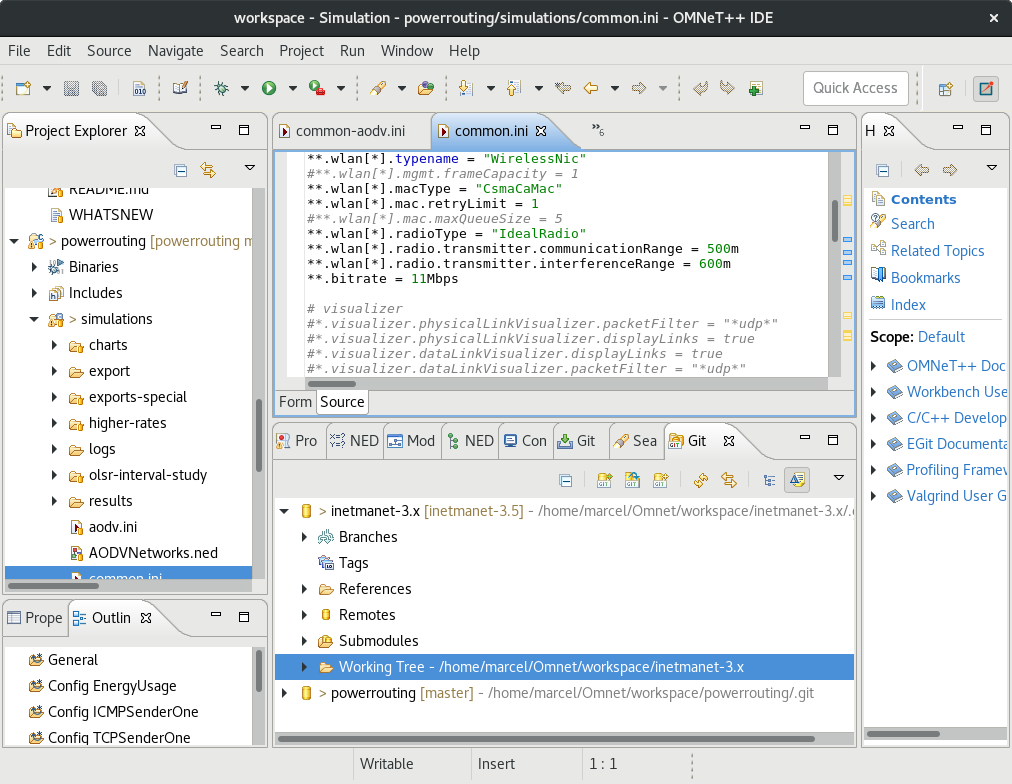
\includegraphics[scale=0.23]{bilder/gui1.png}
  \caption{IDE-GUI von OMNeT++}
  \label{image:omnet:gui}
\end{figure}

\begin{figure}
  \centering
  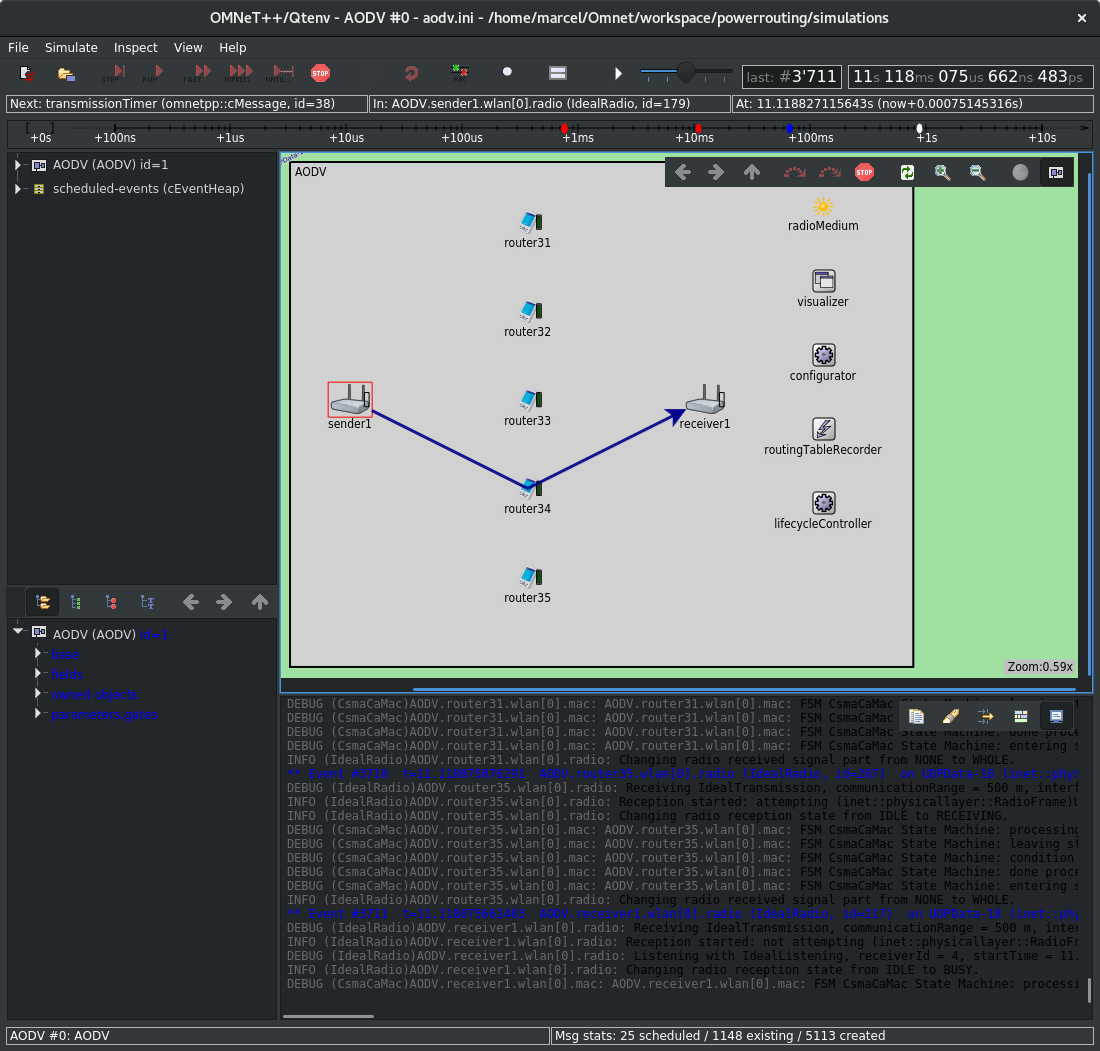
\includegraphics[scale=0.213]{bilder/gui2.png}
  \caption{Simulations-GUI von OMNeT++}
  \label{image:omnet:rungui}
\end{figure}

Die Simulationen erzeugen verschiedene Dateien, in denen alle Werte gemäß der Programmierung gespeichert sind. Des weiteren lassen sich die Nachrichten aller Objekte aufzeichnen. Eine tiefere Beschreibung der Möglichkeiten wird im nächsten Kapitel im Rahmen der Auswertung der Ergebnisse vorgenommen.\newline

Da die Anpassung von \gls{olsr} per Vererbung eine Änderung am Framework erforderlich gemacht hätte, wurden die für die Protokolle \gls{olsr} und \gls{aodv} benötigten Klassen komplett kopiert und in einen \textit{eigenen Namespace} überführt. Dort wurden die angepassten Versionen dann per Vererbung realisiert. Der gesamte Code, der im Rahmen dieser Arbeit erstellt wurde, steht unter der \gls{gpl} auf GitHub zur Verfügung.\footnote{https://github.com/marcelebbrecht/powerrouting} Da bei \gls{olsr} nur die einfachste Version genutzt wird, sind beide Verfahren nah an den jeweiligen \glspl{rfc} und vor allem für die angedachten Versuche hinreichend implementiert. Im Fall von \gls{aodv} scheint es in speziellen Fällen Probleme mit der \textit{loop avoidance} zu geben. Die Ursachen hierfür konnten aber nicht abschließend geklärt werden. Die Implementierung bestehen in der Regel aus folgenden Komponenten:

\begin{itemize}
\item Einer NED für die \textit{Router}, in der die Verwendung des jeweiligen \textit{Routingverfahrens} bestimmt und alle Eigenschaften und Funktionen eines \textit{Wireless Hosts} erbt.
\item Einer NED für das \textit{Protokoll}. Hier wird die Verbindung zu den \textit{C++ Klassen} hergestellt und es werden verschiedene \textit{Einstellungen} definiert.
\item Einer Sammlung aus \textit{C++ Klassen}, welche die Kontrollnachrichten und das Verhalten definieren.
\end{itemize}

\begin{figure}
  \centering
  \footnotesize
  \begin{lstlisting}[frame=single]
# ping sender one
**.sender1.numPingApps = 1
**.sender1.pingApp[0].destAddr = "receiver1(ipv4)"
**.sender1.pingApp[0].sendInterval = 1s
**.sender1.pingApp[0].startTime = 5s

  \end{lstlisting}
  \caption{Auszug INI in OMNeT++}
  \label{listing:omnet:ini}
\end{figure}

Leider sind die Protokolle nicht mit allen verfügbaren \textit{Radio}, \textit{MAC} und \textit{Interface-Typen} kompatibel umgesetzt. Es konnte jedoch eine Schnittmenge gefunden werden, um die Vergleichbarkeit sicherzustellen. Da nur das grundsätzliche Verhalten der Protokolle untersucht werden soll, wurde das verwendete Funkmodell möglichst einfach gewählt. Das Setup für die Simulationen lautet wie folgt:

\begin{itemize}
\item Als Schnittstellen-Typ wird \textit{WirelessNic} genutzt. Dieser stellt eine einfache \gls{wlan} Schnittstelle zur Verfügung.
\item Auf der \gls{maclayer} kommt \textit{CSMA/CA} zur Anwendung.
\item Als Radio-Typ wird \textit{IdealRadio} verwendet. Die Bitrate beträgt 11MBit/s, die Reichweite für die Übertragung 500m, die für Interferenzen 600m. Hierdurch können immer die jeweils direkten Nachbarn erreicht und gestört werden.
\item Zur Realisierung der endlichen Energiequelle und des Verbrauchers wurden die Klassen \textit{IdealEpEnergyStorage} und \textit{StateBasedEpEnergyConsumer} gewählt. Um die Bewertung der Ergebnisse zu vereinfachen, wurde der Energieverbrauch für alle Vorgänge, außer Senden, auf Null gesetzt. Bei den normalen Simulationen starten die Router mit derselben Ladung. Sie Sender und Empfänger verfügen jedoch über einen unbegrenzten Energievorrat.
\item Alle maßgeblichen Versuche wurden in \textit{100 Wiederholungen} mit verschiedenen Zufallszahlen durchgeführt, um eine hinreichende Signifikanz zu erreichen. Die Seeds wurden in der Konfiguration hinterlegt.
\item Die Simulationszeit beträgt in der Regel 180 Sekunden. Da bei kürzerer Laufzeit die Ergebnisse abweichen, wurde eine zusätzliche Auswertung für 60 Sekunden erzeugt um die Unterschiede transparent zu machen.
\item In den meisten Simulationen werden, nach einer \textit{Vorlaufzeit von 10 Sekunden}, \textit{UDP-Nachrichten} mit einem Abstand von circa \textit{50ms} verschickt.
\end{itemize}

\begin{figure}
  \centering
  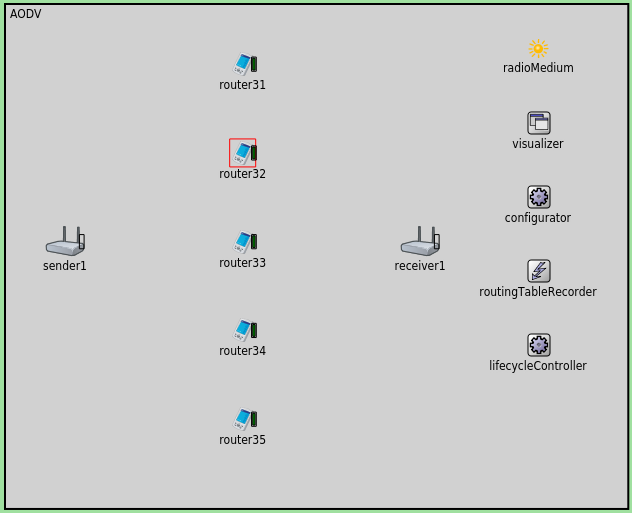
\includegraphics[scale=0.35]{bilder/aodv1.png}
  \caption{Single-Hop Testnetz}
  \label{image:omnet:aodv1}
\end{figure}

\subsection{Simulationsbeschreibung}
\label{chapter:versuch:aufbau:sim}

Für die verschiedenen Simulationen wurden folgende Topologien geschaffen:

\begin{itemize}
\item Ein Single-Hop Netz mit einem Sender, einem Empfänger und 5 Routern in der Mitte, die jeweils den Sender und Empfänger direkt erreichen können (Abbildung \ref{image:omnet:aodv1}).
\item Ein Multi-Hop Netz mit einem Sender, einem Empfänger, mehr Routern und einer geringeren Reichweite. Die Pakete müssen mindestens über 3 Router geleitet werden, bis sie das Ziel erreichen (Abbildung \ref{image:omnet:aodv2}).
\end{itemize}

\begin{figure}
  \centering
  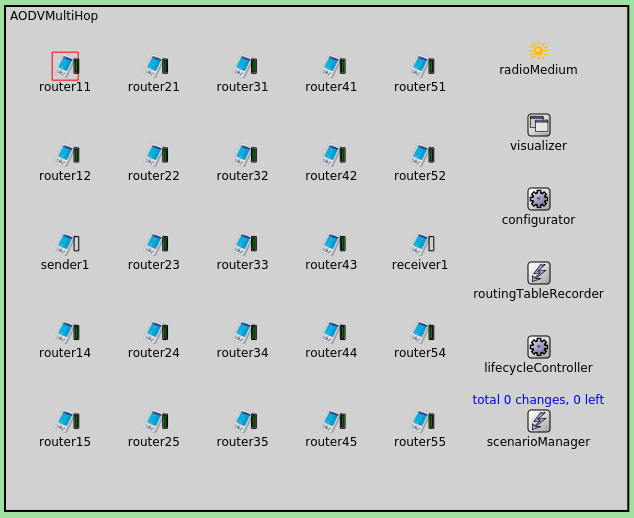
\includegraphics[scale=0.35]{bilder/aodv2.png}
  \caption{Multi-Hop Testnetz}
  \label{image:omnet:aodv2}
\end{figure}

Darüber hinaus gibt es weitere ergänzende Setups, auf welche in der Auswertung näher eingegangen wird: 

\begin{itemize}
\item Abweichende Ladung beim Start
\item Mischung aus angepasstem und normalem \gls{aodv}/\gls{olsr}
\item Eine ParameterStudy
\end{itemize}

\subsection{Neue Metrik}
\label{chapter:versuch:aufbau:metrik}

\begin{figure}
  \centering
  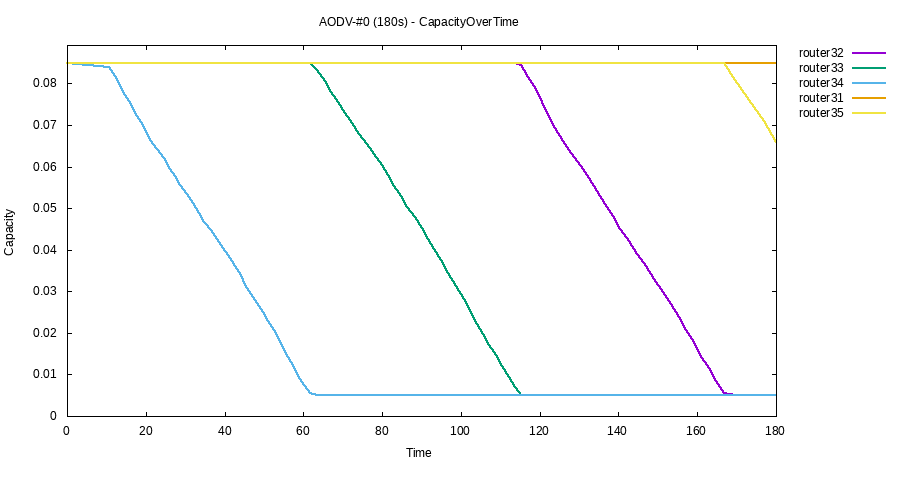
\includegraphics[scale=0.425]{bilder/aodv3.png}
  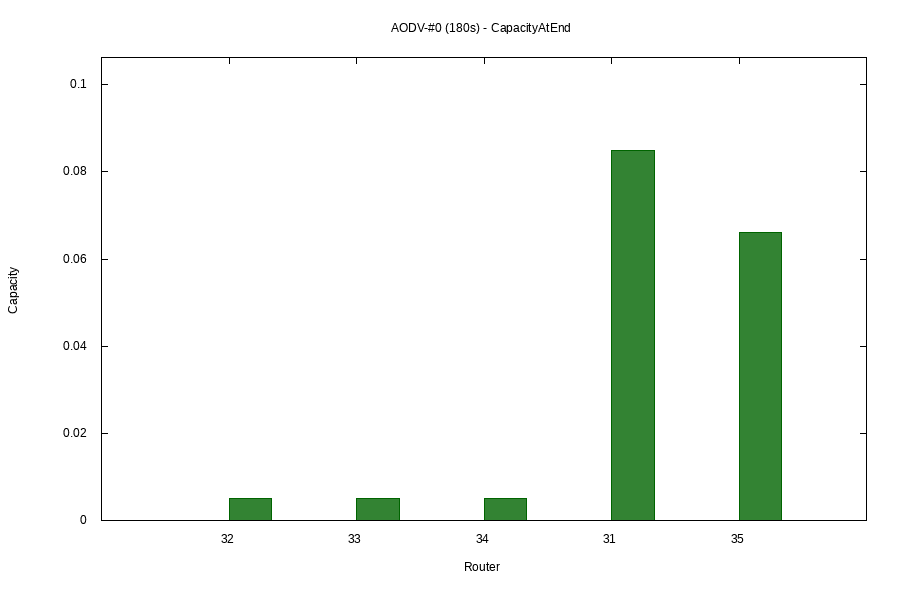
\includegraphics[scale=0.425]{bilder/aodv4.png}
  \caption{Energieverbrauch und -vorrat bei AODV nach 180 Sekunden}
  \label{image:omnet:aodv3}
\end{figure}

Die \glspl{rv} nutzen für die Bewertung der Routen den \textit{HopCount}, wobei bei \gls{olsr} auch die \textit{Willingness} in die Wahl der Gateways einbezogen wird. Um die Kompatibilität mit unangepassten Systemen beibehalten zu können, sollten diese Bewertungsmaßstäbe erhalten werden. Wie bereits in Kapitel \ref{chapter:routing} erwähnt, sollte also bei \gls{aodv} der \textit{HopCount}, bei \gls{olsr} die \textit{Willingness} manipuliert werden. Im Normalfall wird, nachdem einmal eine gültige Route ermittelt wurde, ein Pfad solange genutzt, bis ein Router auf dem Weg nicht mehr zur Verfügung steht. Wenn man davon ausgeht, dass dies nur durch Abschaltung aufgrund von unzureichender Ladung der Energieversorgung geschehen kann, dann wird in solch einem Netz eine Energieversorgung nach der anderen verbraucht (siehe Abbildungen \ref{image:omnet:aodv3}). Es ergibt sich also eine hohe Abweichung zwischen den Endständen. Da es das erklärte Ziel ist, die Weiterleitung von Paketen vom Stand der Energieversorgung der jeweiligen Router abhängig zu machen, muss eine neue Bewertungsmetrik definiert werden, die im weiteren als \textit{Energy fairness} bezeichnet wird. Je geringer die Abweichung der Energiestände am Ende der Simulation, desto \textit{fairer} ist die Verteilung. Die Metrik $M$ entspricht somit der Standardabweichung der Ladestände. Sei $n$ die Anzahl der Router, $C(i)$ die Restladung des jeweiligen Routers $i$ und $\bar{x} = \sum_{i=1}^{n} \frac{C(i)}{n}$ das arithmetische Mittel der Restladungen, dann gilt:
\begin{displaymath}
M = \sqrt{\sum_{i=1}^{n} \frac{(C(i)-\bar{x})^2}{n}} \\
\end{displaymath}
Je geringer dieser Wert ausfällt, desto ausgeglichener ist der Ladezustand und erfolgreicher die Anpassung. Allerdings muss auch berücksichtigt werden, dass Änderungen an den Routen zu Paketverlusten führen können, was bei häufigem Auftreten zu eklatanten Beeinträchtigungen führen kann. Um dies besser bewerten zu können, benötigen wird die \textit{Performance} $F$. Sei $L$ der durchschnittliche PacketLoss der Verbindungen im gesamten Netz und $c=10^{-10}$, dann gilt
\begin{displaymath}
F = ( 1 - ( L + c ) ) / ( M + c )
\end{displaymath}
Der Grad in dem eine Neuberechnung der Verbindungen stattfinden muss, hängt an ein paar spezifischen Einstellungen, welche in den nachfolgenden Abschnitten beschrieben und für die im Rahmen der Simulation mittels der \textit{ParameterStudy} optimale Werte ermittelt wurden.

\subsection{Anpassung AODV-PO (PowerOrientation)}
\label{chapter:versuch:aufbau:anpassungen-aodv}

Um den gewünschten Effekt zu erreichen, müssen die Router regelmäßig ihren Ladezustand überprüfen und dafür sorgen, dass die Routen angepasst werden. Durch das reaktive Design des Protokolls kommt es dabei aber zu kurzzeitigen Ausfällen, da erst eine neue Route ermittelt werden muss. Aus diesem Grund sollte die Anpassung nur nach einer signifikanten Änderung des Ladezustands eintreten. Diese Signifikanz wird im Weiteren als \textit{Trigger} $t$ bezeichnet und zwischen $0{,}1$ und $0{,}9$ gewählt. Sei $C(i)$ der relative Ladezustand des Hosts $i$ zwischen $0$ (leer) und $1$ (voll). Wenn \begin{displaymath}
(C(i) * 100) \mod (100t) = 0
\end{displaymath} 
gilt, wird eine Anpassung durchgeführt. So führt \zB $t=0{,}1$ zu einer Reaktion bei $100\%,90\%,80\%, ...$, also alle $10\%$. In diesem Fall wird ein \gls{rerr} erzeugt und nach dem bekannten Schema verschickt, damit eine Neubestimmung der Routen beginnt. Ferner soll es möglich sein den Grad der Veränderung anzupassen, was als \textit{Sensitivity} $s$ bezeichnet wird und zwischen $0{,}1$ und $10$ gewählt werden kann. Mit ihr kann bestimmt werden, wie stark der HopCount erhöht werden soll. Dieser Aufschlag wird als \textit{Penalty} $P$ bezeichnet. Im Normalfalls berechnet ein Router, der eine Verbindung per \gls{rrep} weitergibt den neuen HopCount $H_{neu}$ wie folgt aus dem ihm bekannten Wert $H_{alt}$:
\begin{displaymath}
H_{neu} = H_{alt} + 1
\end{displaymath}
In der angepassten Version wird in die Berechnung des neuen HopCounts $H'_{neu}$ die Penalty $P$ einbezogen, sofern der Router über einen begrenzten Energievorrat verfügt. Ferner kann in so einem Fall ein fester Aufschlag $B$ definiert werden, damit immer mit einer höheren Penalty agiert wird. Es gilt:
\begin{displaymath}
H'_{neu} = H_{alt} + 1 + P
\end{displaymath}
wobei die Penalty folgendermaßen berechnet wird:
\begin{displaymath}
P = \lceil\frac{s}{C_i} + B\rceil
\end{displaymath}
Bei $C(i) = 0{,}8$, $s = 2$ und $B=0$ ergibt sich also $P=\lceil\frac{2}{0{,}8} + 0\rceil = \lceil2{,}5\rceil = 3$ und somit $H'_{neu} = H_{alt} + 1 + 3 > H_{neu} = H_{alt} + 1$. Daraus folgt $H'_{neu} - H_{neu} = 3$, somit ist der Aufschlag durch den Router um 3 Hops höher. Er stellt sich also erheblich schlechter dar als er ist, damit andere Router \ggf andere Wege wählen sofern diese zur Verfügung stehen. Allerdings sollte $s$ mit Bedacht gewählt werden, da der Wert bei hohem $s$ und niedrigem $C(i)$ schnell steigt (er beträgt \zB für $s=10, C(i)=0.1$ bereits $100$) und die Anzahl maximaler Hops \textit{einer gesamten Route} auf 255 begrenzt ist. Daher sollte $s$ immer in Abhängigkeit der Größe des Netzes gewählt werden.\newline

Die Grundeinstellungen des Protokolls sind in OMNeT++ nach den Empfehlungen der RFC gesetzt und so belassen.

\subsection{Anpassung OLSR-PO (PowerOrientation)}
\label{chapter:versuch:aufbau:anpassungen-olsr}

Bei \gls{olsr} erfolgt die Anpassung auf ähnliche Art. Der Unterschied besteht allerdings in der Anwendung: Statt die Routen wie bei \gls{aodv} zu unterbrechen, wird die \textit{Willingness} der Hosts heruntergesetzt. Dies führt zwar zu einer gewissen Verzögerung bis die Routen geändert werden, allerdings entsteht keine Unterbrechung der Verbindungen. Stattdessen findet ein fließender Übergang statt. Daher ist \gls{olsr} durch geringeren \textit{PacketLoss} im Vorteil. Auch hier gibt es, aus den gleichen Gründen, einen Trigger $t$, der wie bei \gls{aodv} definiert ist. Der Grad der Veränderung, was erneut als \textit{Sensitivity} $s$ bezeichnet wird und zwischen $0{,}01$ und $0{,}99$ gewählt werden kann, bestimmt, wie stark die Willingness $W$ herabgesetzt wird. Auch hier erfolgt die Anpassung nur, wenn der Router über einen begrenzten Energievorrat verfügt. Ferner kann in so einem Fall ein fester Aufschlag $B$ definiert werden, damit immer mit einer höheren Penalty agiert wird. Es gilt:
\begin{displaymath}
W_{neu} = \lfloor\max(1,(7\cdot C(i)\cdot (1-s)-B))\rfloor
\end{displaymath}
Bei $C(i) = 0{,}8$, $s = 0{,}2$ und $B=0$ ergibt sich also $W_{neu} = \lfloor\max(1,(7\cdot 0{,}8\cdot (1-0{,}2)-0))\rfloor = \lfloor\max(1,4{,}48)\rfloor = 4$. Somit wird die Willingness auf den Wert 4 gesetzt. Hierdurch ist es möglich, dass Mitglieder der \glspl{1hnb}, die den Host als \gls{mpr} nutzen, auf einen anderen Host mit höherer Willingness als \gls{mpr} umstellen und somit der Verkehr über einen anderen Router geleitet wird, sofern dieser zur Verfügung steht. Auch hier sollte $s$ mit Bedacht gewählt werden, da bei hohem $s$ die Willingness sehr schnell sinkt.\newline

Die Grundeinstellungen des Protokolls wurden in OMNeT++ für die angepasste Version folgendermaßen gesetzt:
\begin{itemize}
\item \textbf{HELLO-Interval}: $2s$
\item \textbf{TC-Interval}: $5s$
\item \textbf{MID-Interval}: $5s$
\item \textbf{OLSR\_REFRESH-Interval}: $2s$
\end{itemize}

In der ursprünglichen Version wird statt dessen ein HELLO- und OLSR\_REFRESH-Interval von $0.5$ Sekunden genutzt. Dies erhöht zwar den Overhead, reduziert aber den Paketverlust durch ausgefallene Router drastisch.


% routing.tex
% Kapitel 5: Auswertung

\chapter{Auswertung}
\label{chapter:auswertung}

\section{Eingesetze Technik}
\label{chapter:auswertung:technik}

Leider verfügt die in OMNeT++ enthaltene Software nicht über die Möglichkeiten, aufgezeichnete Daten in hinreichender Tiefe oder großer Menge effizient auszuwerten und erzeugt zudem regelmäßig Abstürze und falsche Ergebnisse. Somit musste ein anderer Weg gewählt werden: Die von OMNet++ erzeugten Messdaten wurden mittels \textit{scavetool}, das zum Lieferumfang gehört, nach \textit{CSV} exportiert. Nach einer weiteren Aufbereitung der Daten durch \textit{PERL}, wie dem Entfernen von nicht benötigten Dezimalstellen und der Reduzierung der Datenmenge durch einen Dropout, wurden diese mittels \textit{GnuPlot} visualisiert. Zwecks besserer Lesbarkeit wird in diesem Kapitel der Punkt als Dezimaltrennzeichen verwendet.

\begin{figure}
  \centering
  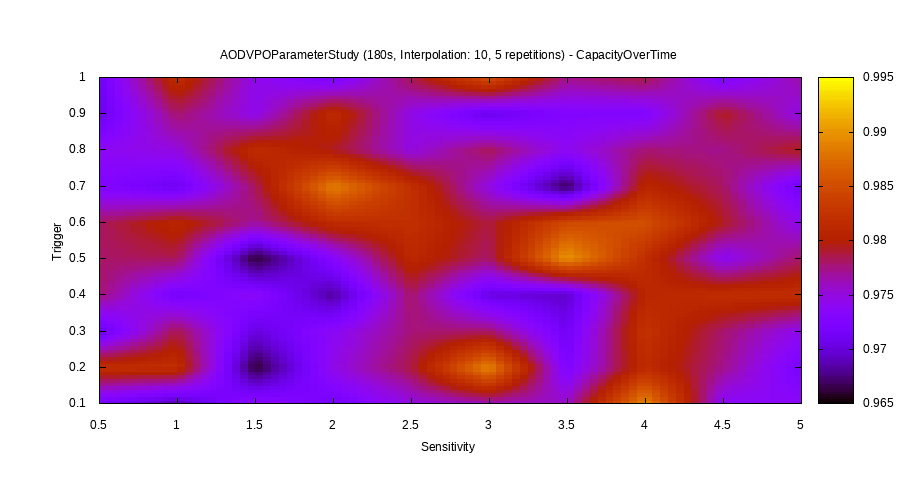
\includegraphics[scale=0.45]{bilder/aps1.png} \\
  \caption{ParameterStudy AODV nach 180 Sekunden, Abweichung der Kapazität}
  \label{image:omnet:aodv:one}
\end{figure}

\section{Die Auswertung}
\label{chapter:auswertung:versuche}

\subsection{Parameter Study}
\label{chapter:auswertung:study}

Wie zuvor beschrieben, gibt es bei beiden Protokollen die Möglichkeit die Stärke und Frequenz der Anpassung der Routingeigenschaften über Parameter zu steuern, namentlich Trigger $t$ und Sensitivität $s$. Um hierfür geeignete Werte zu ermitteln, wurde eine \textit{ParameterStudy} entworfen, die mögliche Kombinationen beider Werte in 5\% Schritten des gültigen Intervalls in mehrfacher Wiederholung testet. Die Werte dazwischen wurden interpoliert. Grundsätzlich sehen Diagramme in 3D natürlich besser aus, dennoch sind sie für eine fundierte Analyse weniger hilfreich als \textit{Heatmaps}. Daher werden im weiteren Verlauf nur Letztere gezeigt. Für alle im Rahmen der ParameterStudy gezeigten Diagramme gilt: Je höher der Wert, desto besser das Ergebnis.


\begin{figure}
  \centering
  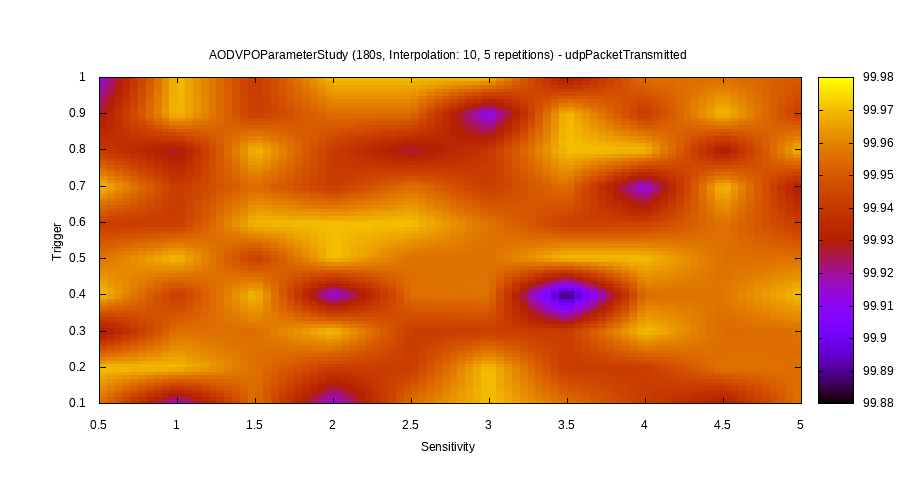
\includegraphics[scale=0.45]{bilder/aps2.png} \\
  \caption{ParameterStudy AODV nach 180 Sekunden, PacketLoss}
  \label{image:omnet:aodv:two}
\end{figure}

\subsubsection{Parameter Study - AODV}
\label{chapter:auswertung:studyaodv}

\begin{figure}
  \centering
  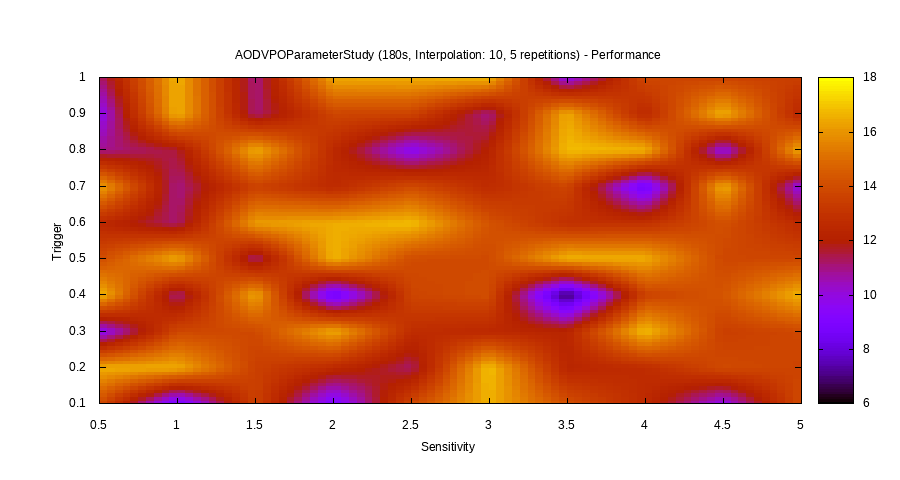
\includegraphics[scale=0.45]{bilder/aps3.png} \\
  \caption{ParameterStudy AODV nach 180 Sekunden, Performance}
  \label{image:omnet:aodv:three}
\end{figure}

In Abbildung \ref{image:omnet:aodv:one} wird die Beziehung $1-D(s,t)$ visualisiert, wobei $D$ die \textit{Standardabweichung der Kapazität} zum Ende der Simulation darstellt. Je heller der Wert, desto ähnlicher waren die Ladestände der Router. Es muss jedoch auch die Verlustrate betrachtet werden, denn was nützt ein ausgeglichener Verbrauch, wenn keine Daten mehr transportiert werden. Die Auswertung des \textit{PacketLoss} $L$ kann der Abbildung \ref{image:omnet:aodv:two} entnommen werden, wobei hier wieder $1-L(s,t)$ dargestellt wird. Wenn man beide Tests miteinander in Form der \og \textit{Performance} kombiniert, dann ergibt sich daraus Abbildung \ref{image:omnet:aodv:three}. Aus den vorliegenden Daten können nun mehrere Parameterkombinationen ermittelt werden, die zu guten Ergebnissen führen müssten, also durch eine hohe Performance sowohl einen ausgeglichenen Ladezustand herstellen, als auch mit einem geringen PacketLoss auskommen. Für die weiteren Untersuchungen wurde das Tupel $(s,t) = (4,0.3)$ gewählt. Die Auswertung des \textit{Overhead} durch das Protokoll in Abbildung \ref{image:omnet:aodv:six} zeigt, dass auch hier sehr gute Werte, die gewählte Kombination gehört zum besten Drittel, erreicht werden. Daher wurden die genannten Werte für fast alle weiteren Simulationen genutzt. Es liegen auch viele optimale Kombinationen in den Randbereichen, bei deren Verwendung kam es jedoch bei einigen Iterationen immer wieder zu ungewöhnlichen Abweichungen, die vermutlich auf ungünstige Zufallswerte zurückzuführen sind.

\begin{figure}
  \centering
  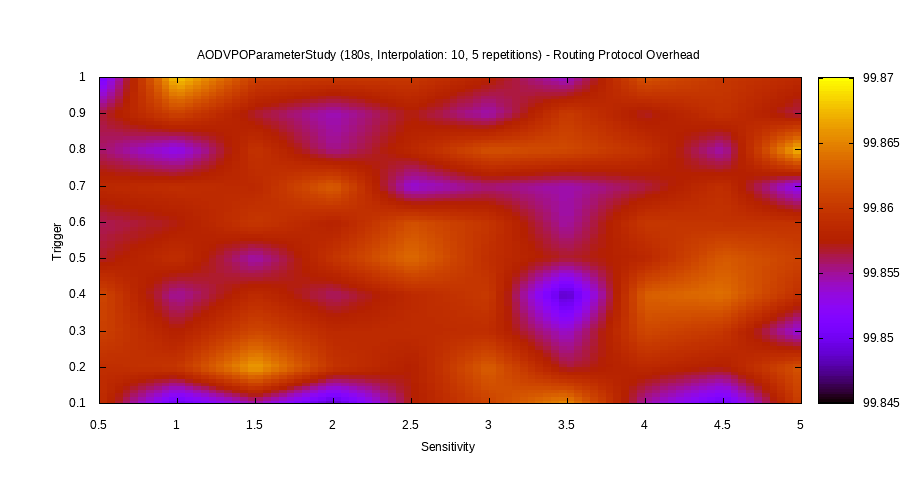
\includegraphics[scale=0.45]{bilder/aps6.png} \\
  \caption{ParameterStudy AODV nach 180 Sekunden, Routing Overhead}
  \label{image:omnet:aodv:six}
\end{figure}

\subsubsection{Parameter Study - OLSR}
\label{chapter:auswertung:studyaodv}

Hier wurden die selben Untersuchungen durchgeführt. Die Ergebnisse sind den Abbildungen \ref{image:omnet:olsr:one}, \ref{image:omnet:olsr:two}, \ref{image:omnet:olsr:three} und \ref{image:omnet:olsr:six} zu entnehmen. Es gelten die selben Aussagen wie bei \gls{aodv}. Während jedoch bei \gls{aodv} die Abweichung bis zum sechsfachen zwischen dem besten und schlechtesten Ergebnis beträgt, ist diese bei \gls{olsr} deutlich geringer, wie sich den Abbildungen entnehmen lässt. Es wurde das Tupel $(s,t) = (0{.}375 ,0{.}3)$ gewählt, da es akzeptable Ergebnisse liefert.

\begin{figure}
  \centering
  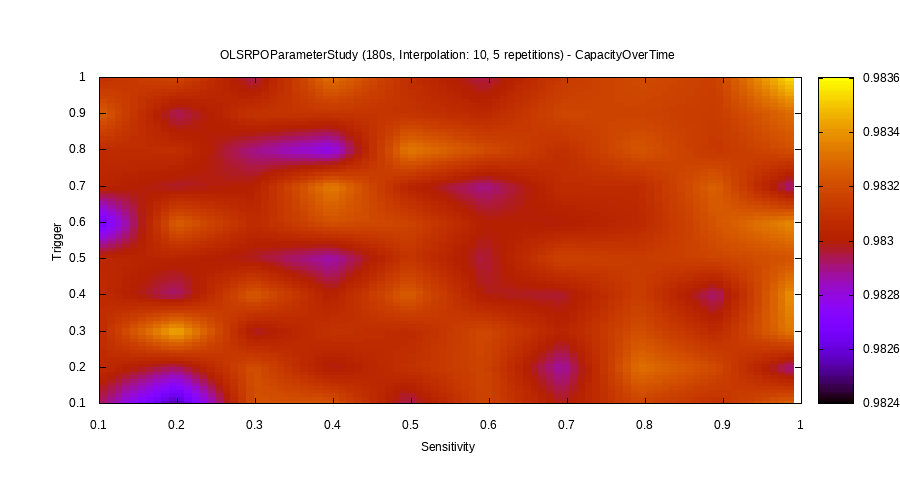
\includegraphics[scale=0.45]{bilder/ops1.png} \\
  \caption{ParameterStudy OLSR nach 180 Sekunden, Abweichung der Kapazität}
  \label{image:omnet:olsr:one}
\end{figure}

\begin{figure}
  \centering
  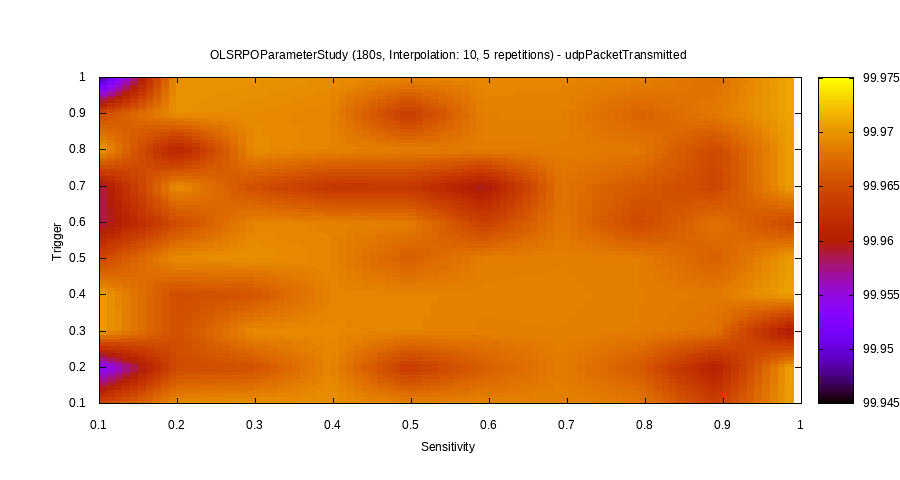
\includegraphics[scale=0.45]{bilder/ops2.png} \\
  \caption{ParameterStudy OLSR nach 180 Sekunden, PacketLoss}
  \label{image:omnet:olsr:two}
\end{figure}

\begin{figure}
  \centering
  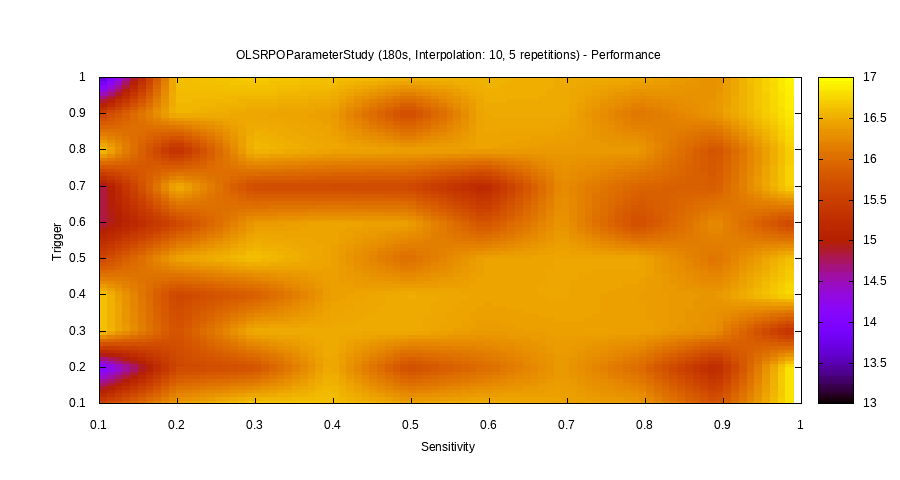
\includegraphics[scale=0.45]{bilder/ops3.png} \\
  \caption{ParameterStudy OLSR nach 180 Sekunden, Performance}
  \label{image:omnet:olsr:three}
\end{figure}

\begin{figure}
  \centering
  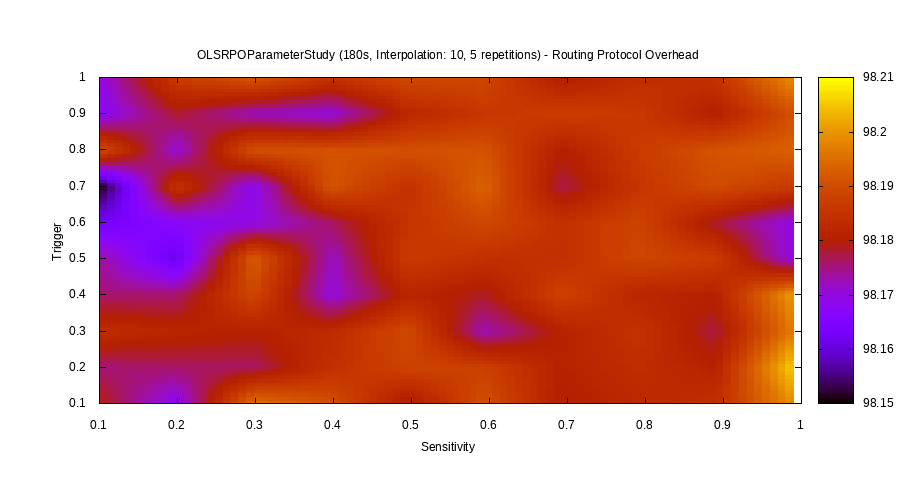
\includegraphics[scale=0.45]{bilder/ops6.png} \\
  \caption{ParameterStudy OLSR nach 180 Sekunden, Routing Overhead}
  \label{image:omnet:olsr:six}
\end{figure}

\subsection{Auswertung AODV-PO}
\label{chapter:auswertung:versuche-aodv}

Zum Vergleich der Optimierung wurde zuerst ein Single-Hop Netz (\vgl Abbildung \ref{image:omnet:aodv1}) getestet, das ausschließlich aus normalen AODV-Routern besteht. Alle Versuche wurden 100 mal mit verschiedenen Zufallszahlen wiederholt. Die Ladung der Energieversorgungen im Verlauf der Zeit ist in Abbildung   \ref{image:omnet:olsr:av1} dargestellt. Wie man sieht, wird hier immer die komplette Energie eines Routers verbraucht. Anschließend schaltet der Router ab und der nächste Router wird genutzt. Nach der Anpassung stellt sich der Energieverbrauch wie in Abbildung \ref{image:omnet:olsr:av5} dar: Nachdem eine gewisse Menge Energie verbraucht wurde, wird ein \gls{rerr} ausgelöst. Anschließend wird ein anderer Router genutzt, da er als günstigerer Pfad erkannt wird. So wird nach und nach immer wieder der Router gewechselt und der Energieverbrauch gleichmäßig verteilt.\newline

\begin{figure}
  \centering
  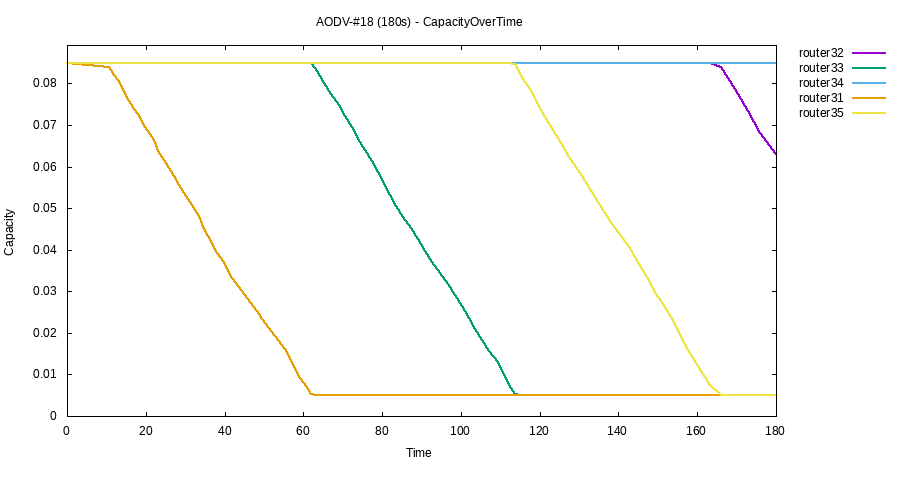
\includegraphics[scale=0.45]{bilder/av1.png} \\
  \caption{Verlauf Ladezustand bei AODV, 180 Sekunden}
  \label{image:omnet:olsr:av1}
\end{figure}

\begin{figure}
  \centering
  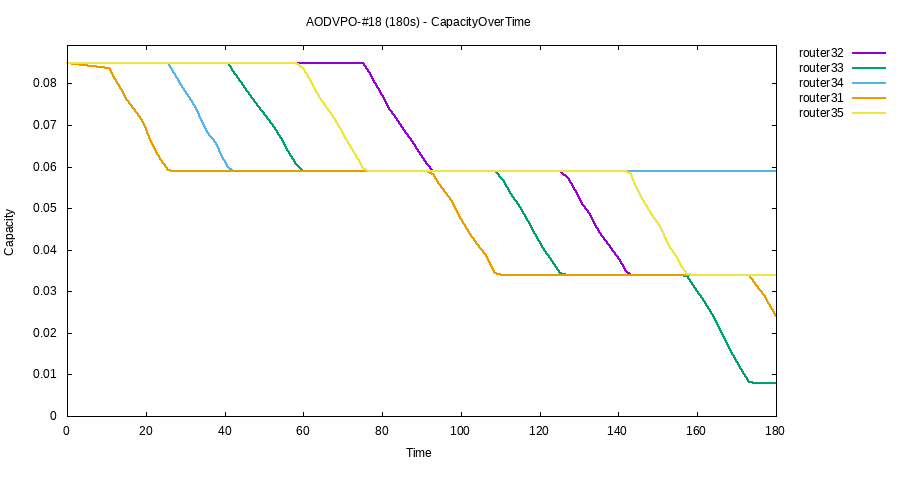
\includegraphics[scale=0.45]{bilder/av5.png} \\
  \caption{Verlauf Ladezustand bei AODV-PO, 180 Sekunden}
  \label{image:omnet:olsr:av5}
\end{figure}

Um die Wirkung eines geänderten Triggers $t$ zu testen, wurden zwei Versuche mit $t = 0.2$ (schnellere Reaktion) und $t=0.4$ (langsamere Reaktion) durchgeführt. Wie man in den Abbildungen \ref{image:omnet:olsr:av9} und \ref{image:omnet:olsr:av10} erkennen kann, werden hier die Router öfter \bzw seltener gewechselt.\newline

\begin{figure}
  \centering
  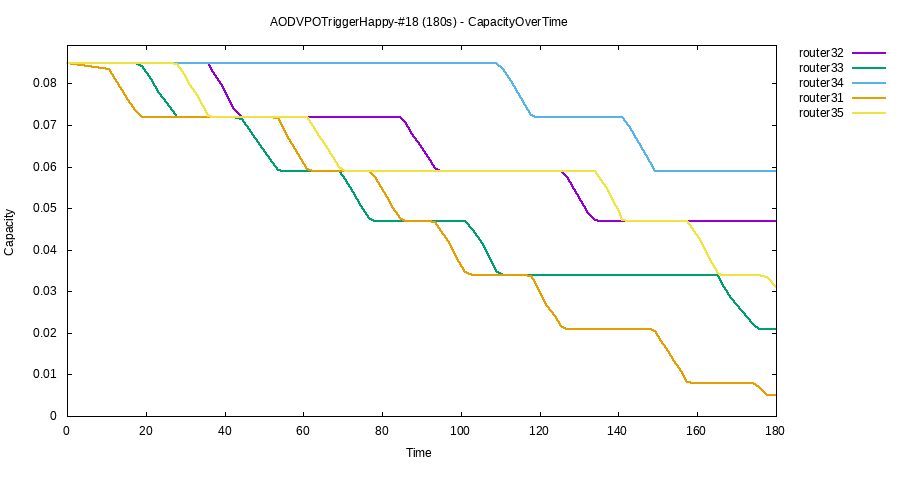
\includegraphics[scale=0.45]{bilder/av9.png} \\
  \caption{Niedrigerer Trigger $t=0.2$ bei AODV-PO, 180 Sekunden}
  \label{image:omnet:olsr:av9}
\end{figure}

\begin{figure}
  \centering
  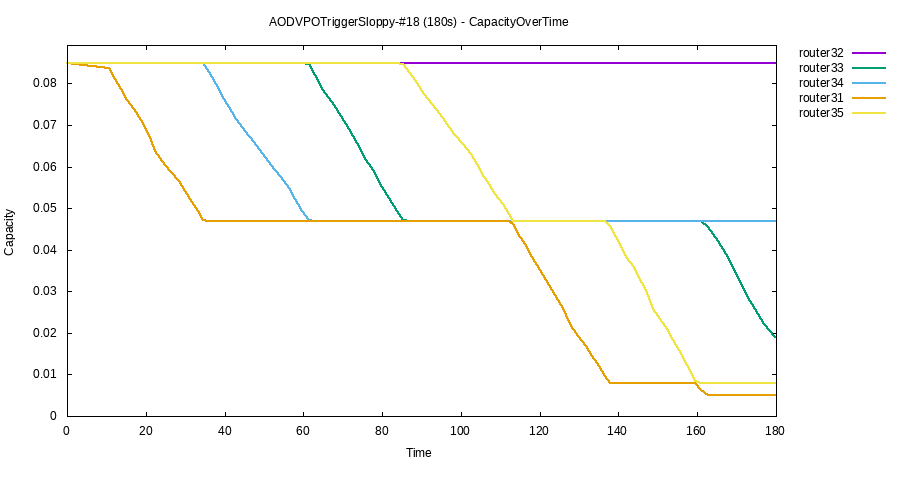
\includegraphics[scale=0.45]{bilder/av10.png} \\
  \caption{Höherer Trigger $t=0.4$ bei AODV-PO, 180 Sekunden}
  \label{image:omnet:olsr:av10}
\end{figure}

Zur Prüfung der Kompatibilität zwischen beiden Varianten des Protokolls wurde eine weitere Simulation durchgeführt. In dem Netz aus Abbildung \ref{image:omnet:olsr:netmixed} arbeiten die Router 22,23,24,42,43,44 mit normalem \gls{aodv}, die anderen mit der angepassten Version. Es funktioniert grundsätzlich, jedoch wird der Verkehr nicht so gleichmäßig wie bei den anderen Untersuchungen verteilt (\vgl Abbildung \ref{image:omnet:olsr:av11}). Auch ein Start mit unterschiedlichen Ladezuständen ist möglich. Der Verkehr wird so verteilt, dass sich diese angleichen.\newline

\begin{figure}
  \centering
  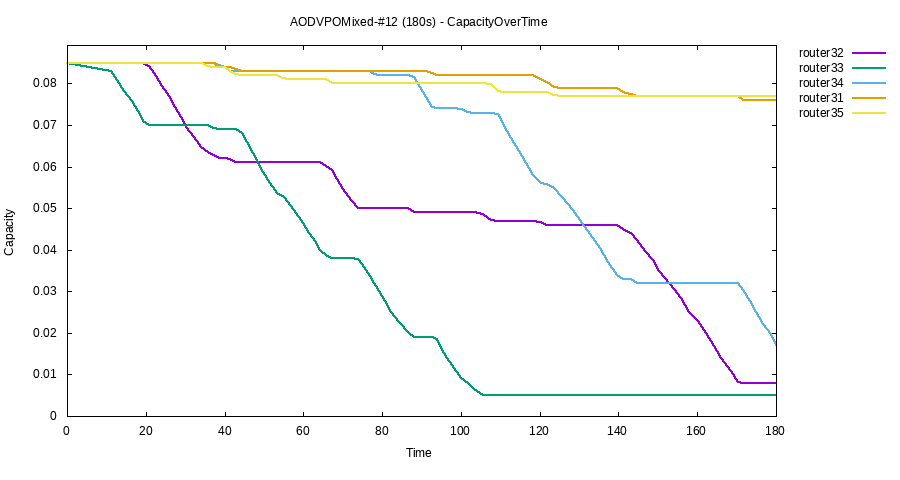
\includegraphics[scale=0.45]{bilder/av11.png} \\
  \caption{AODV und AODV-PO im Mischbetrieb, 180 Sekunden}
  \label{image:omnet:olsr:av11}
\end{figure}

\begin{figure}
  \centering
  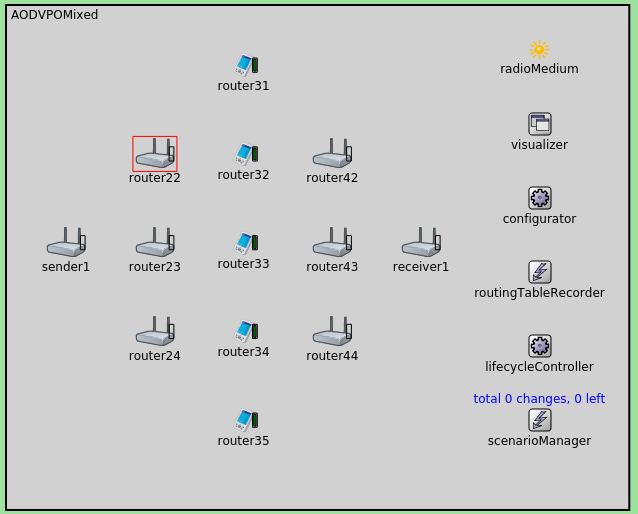
\includegraphics[scale=0.35]{bilder/netmixed.png} \\
  \caption{Netzwerk für den Mischbetrieb}
  \label{image:omnet:olsr:netmixed}
\end{figure}

Das Ziel, den Verkehr nach dem Energievorrat zu verteilen, kann als erreicht angesehen werden. Die erwünschte Kompatibilität zwischen neuem und altem Verfahren ist ebenfalls gegeben.

\subsection{Auswertung OLSR-PO}
\label{chapter:auswertung:versuche-olsr}

Für den Test der Anpassung bei \gls{olsr} wurden die selben Simulationen unter den selben Bedingungen durchgeführt. Die Ergebnisse zeigen das gleiche Verhalten wie bei \gls{aodv}. Die grafischen Auswertungen sind hier zu Gunsten der Übersichtlichkeit nicht dargestellt, sondern dem Anhang \ref{appendix:olsr} zu entnehmen. Das angestrebte Verhalten ist hier ebenfalls erreicht worden.

\subsection{Vergleich Protokolle}
\label{chapter:auswertung:vergleich}

Während die Abweichung der Ladezustände bei beiden Protokollen in der Standardversion vergleichbar hoch ist (Abbildung \ref{image:omnet:olsr:comp1}), erkennt man wie diese bei den angepassten Varianten im Durchschnitt stark abnimmt, bei \gls{olsr} sogar deutlicher. Bemerkenswert ist auch, dass die trägere Version besser als die normale ist, was jedoch mit der Laufzeit erklärbar ist (durch Zufall haben alle Ladezustände den selben Wert). Bei kürzerer oder längerer Laufzeit ergeben sich andere Werte. Der stärkere Grad der Verteilung bei dem proaktiven Verfahren fordert allerdings höheren Overhead (Abbildung \ref{image:omnet:olsr:comp2}).\newline

\begin{sidewaysfigure}
  \centering
  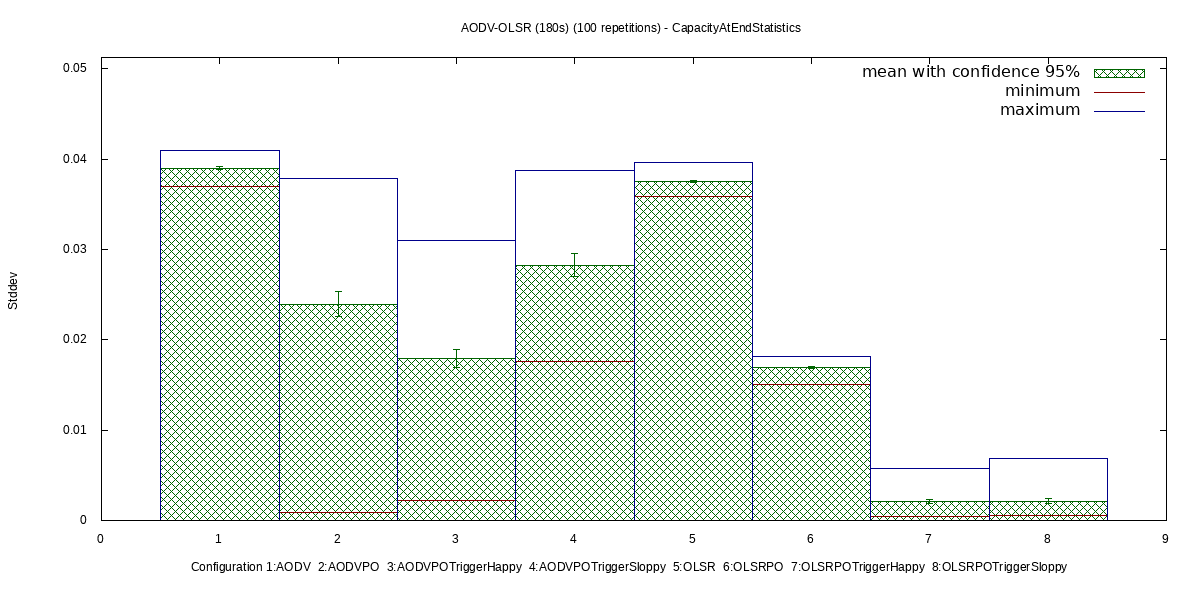
\includegraphics[scale=0.5]{bilder/c1.png} \\
  \caption{Vergleich Verlauf Ladezustand bei OLSR und AODV, 180 Sekunden}
  \label{image:omnet:olsr:comp1}
\end{sidewaysfigure}


\begin{sidewaysfigure}
  \centering
  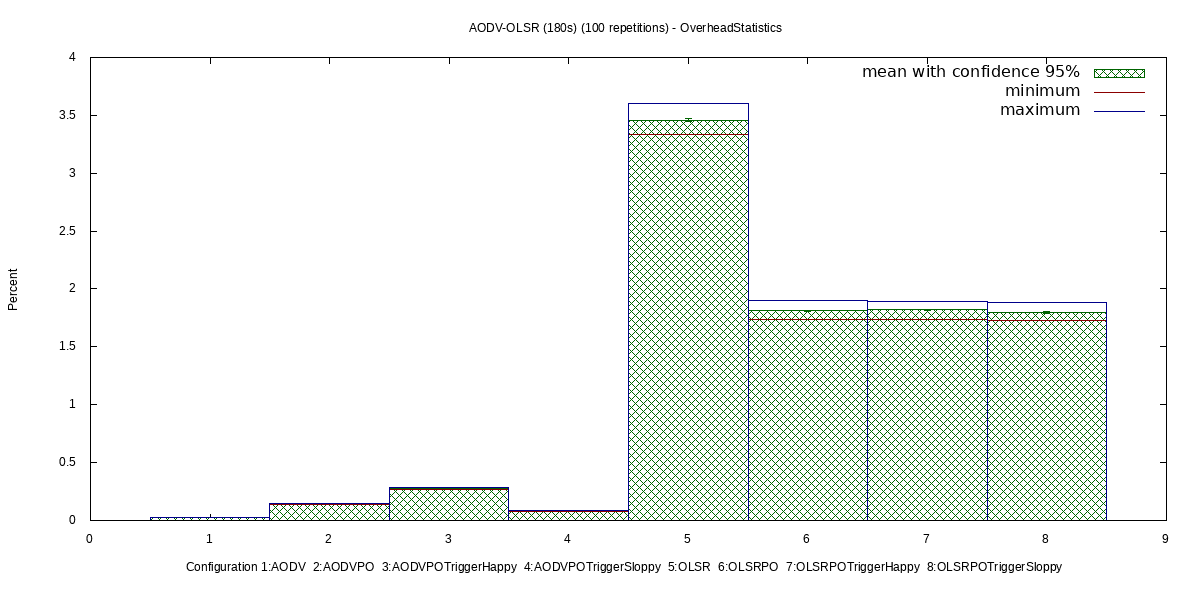
\includegraphics[scale=0.5]{bilder/c2.png} \\
  \caption{Vergleich Overhead bei OLSR und AODV, 180 Sekunden}
  \label{image:omnet:olsr:comp2}
\end{sidewaysfigure}

Der Paketverlust liegt bei den angepassten Varianten deutlich niedriger. Hier liegt \gls{olsr} zudem erheblich vor \gls{aodv}, was durch den nahtlosen Wechsel erklärt werden kann (\vgl Abbildung \ref{image:omnet:olsr:sa3} und \ref{image:omnet:olsr:so3}). Der Ausreißer bei unangepasstem OLSR ist darauf zurückzuführen, dass die Router unkontrolliert abschalten, wodurch es erst eine Weile dauert, bis wieder neue Routen gewählt werden und in der Zwischenzeit Pakete verloren gehen.

\begin{figure}
  \centering
  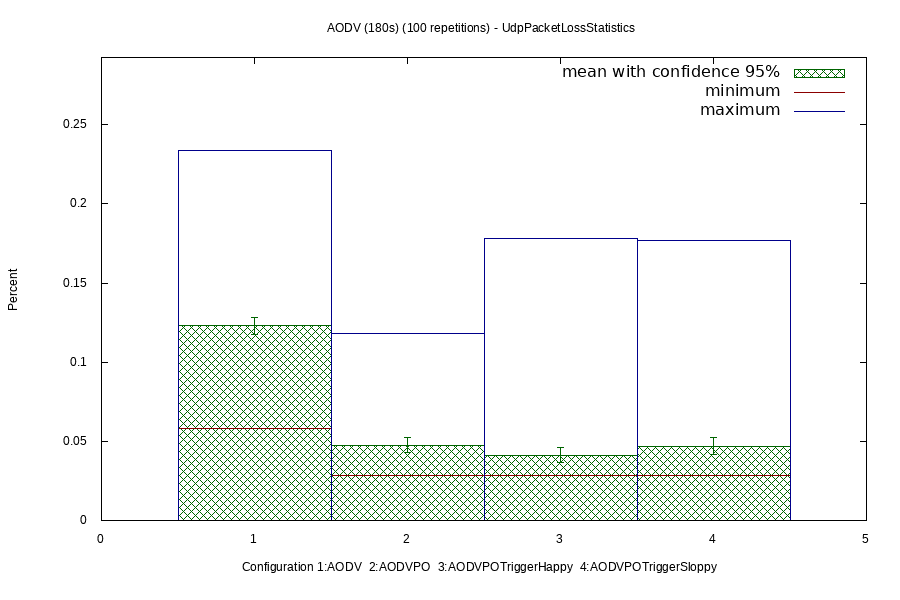
\includegraphics[scale=0.4]{bilder/sa3.png} \\
  \caption{Vergleich PacketLoss bei AODV, 180 Sekunden}
  \label{image:omnet:olsr:sa3}
\end{figure}

\begin{figure}
  \centering
  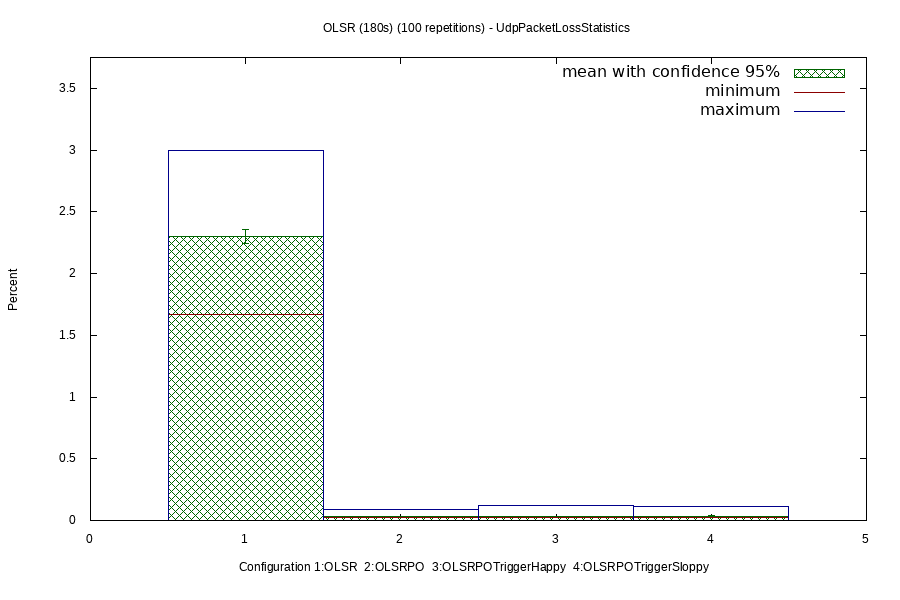
\includegraphics[scale=0.4]{bilder/so3.png} \\
  \caption{Vergleich PacketLoss bei OLSR, 180 Sekunden}
  \label{image:omnet:olsr:so3}
\end{figure}

\subsection{Weitere Erkenntnisse}
\label{chapter:auswertung:erkenntnisse}

Die Simulation wurden mit hundert Wiederholungen durchgeführt. Es zeigt sich, dass die Anpassungen beider Protokolle stabil Ihre Wirkung entfalten. Auch hierzu sind im Anhang \ref{appendix:repeat} entsprechende Auswertungen beigefügt. Es fällt auf, dass die Ergebnisse bei \textit{OLSR-PO} stärker streuen, dennoch sind diese konstant niedriger als bei \gls{olsr}. Darüber hinaus wurde das Verhalten in einem größeren Netz (Abbildung \ref{image:omnet:aodv2}) überprüft. Die Funktion ist dort ebenfalls gegeben, auch wenn es zu stärkeren Abweichungen kommt. \textit{AODV-PO} verhält sich zum Ende der Simulation instabil, die Ursache hierfür konnte nicht abschließend geklärt werden. Hierzu sind entsprechende Auswertungen im Anhang \ref{appendix:multihop} zu finden. Bei der letzten Untersuchung galt es, den Vorteil von proaktiven Protokollen bei vielen verschiedenen Zielen zu untersuchen. Hierzu wurden die Pakete zufällig auf alle Hosts im MultiHop-Netz verteilt. Hier zeigt OLSR ein leicht geringere Verlustrate von Paketen, da die Routen sofort zur Verfügung stehen und nicht erst ermittelt werden müssen, was zu Zeitüberschreitungen und damit zum Verwerfen der Pakete führt (Abbildung \ref{image:omnet:olsr:comp3}). Es ist anzunehmen, dass dieser Vorteil mit wachsender Größe des Netzes zunehmen wird.

\begin{sidewaysfigure}
  \centering
  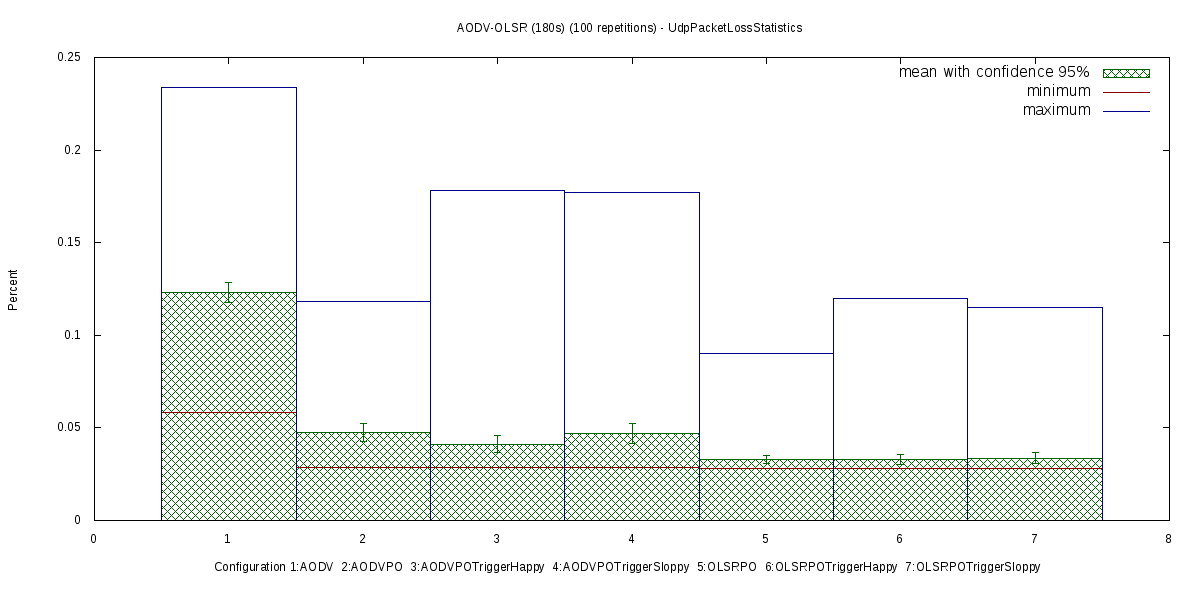
\includegraphics[scale=0.5]{bilder/c3.png} \\
  \caption{Vergleich Verlustrate Multi-Recipient bei OLSR und AODV, 180 Sekunden}
  \label{image:omnet:olsr:comp3}
\end{sidewaysfigure}
% schluss.tex
% Kapitel 6: Fazit

\chapter{Fazit}
\label{chapter:fazit}

Es mag der Eindruck entstehen, dass die Auswertung ein wenig kurz geraten ist. Vielleicht liegt das aber auch daran, das es relativ gut funktioniert. Das gesteckte Ziel, eine faire Verteilung des Verkehrs zu erreichen, wurde, zumindest in den Kernexperimenten, erreicht. Die Funktion ist zudem in gemischten Netzen gegeben. Die Anpassung der Implementierung ist, sowohl im Simulator, als auch für echte Systeme relativ simpel gehalten, damit ein Test unter realen Bedingungen angebracht erscheint. Der Code beider Protokolle ist für den Linux-Kernel frei verfügbar \footnote{https://github.com/erimatnor/aodv-uu} \footnote{https://wiki.freifunk.net/Glossar\#OLSR}. Es stellt sich allerdings die Frage ob es sinnig ist diese beiden sehr alten Protokolle weiter zu entwickeln. Stattdessen erscheint es als sinnvoll diese Anpassungen bei moderneren Verfahren wie \textit{DANE} oder anderen auf den Stromverbrauch optimierten Protokollen zu testen. Wenn ein stromsparendes Verfahren zusätzlich noch den Verkehr fair verteilt, dann kann diese Technologie bei dem Aufbau moderner Ad-Hoc-Infrastrukturen durchaus zu höherer Akzeptanz für den Einsatz auf mobilen Geräten führen. Ich halte es persönlich für sehr realistisch, dass \gls{mesh} in kommenden Mobilfunkgenerationen eine erhebliche Rolle spielen wird. Nicht zuletzt weil es den Providern einen wirtschaftlichen Vorteil bringt.
% Anhang
\appendix
% anhang.tex
% Weitere Informationen zum Projekt und zur Arbeit

\chapter{Auswertungen OLSR}
\label{appendix:olsr}
\begin{center}
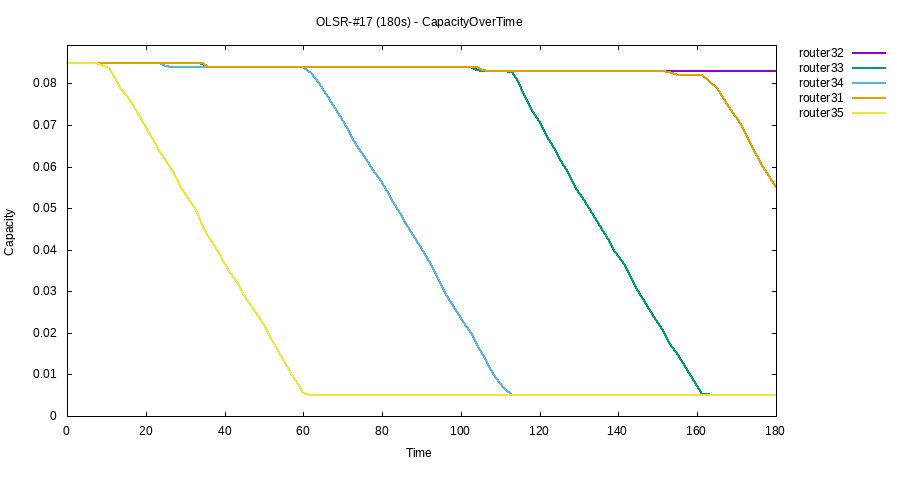
\includegraphics[scale=0.4]{bilder/os1.png} 
\captionof{figure}{Verlauf Ladezustand bei OLSR, 180 Sekunden}
\end{center}

 \newpage 
\begin{center}
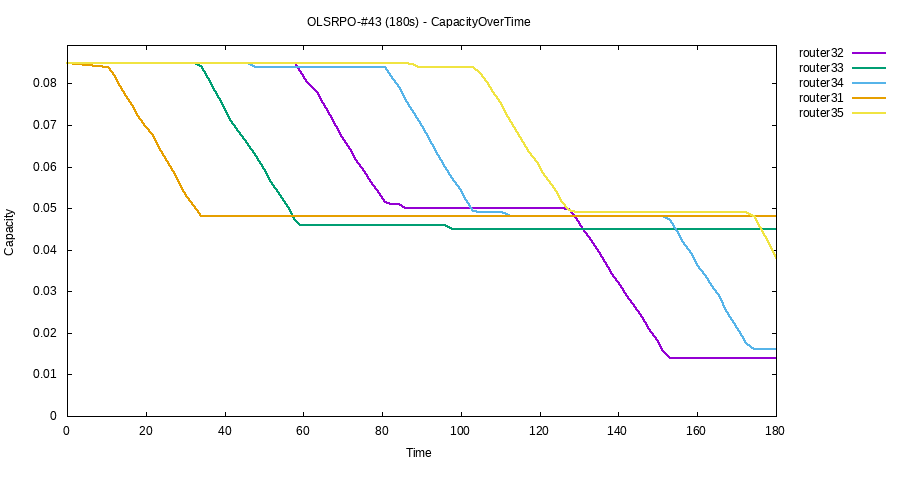
\includegraphics[scale=0.4]{bilder/os2.png} 
\captionof{figure}{Verlauf Ladezustand bei OLSR-PO, 180 Sekunden}
\end{center}

\begin{center}
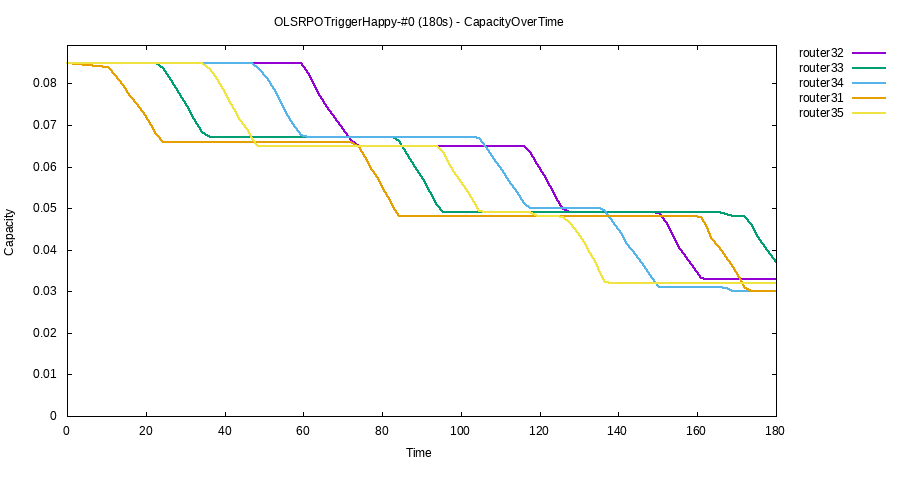
\includegraphics[scale=0.4]{bilder/os3.png}
\captionof{figure}{Niedrigerer Trigger $t=0.2$ bei OLSR-PO, 180 Sekunden}
\end{center}

\newpage

\begin{center}
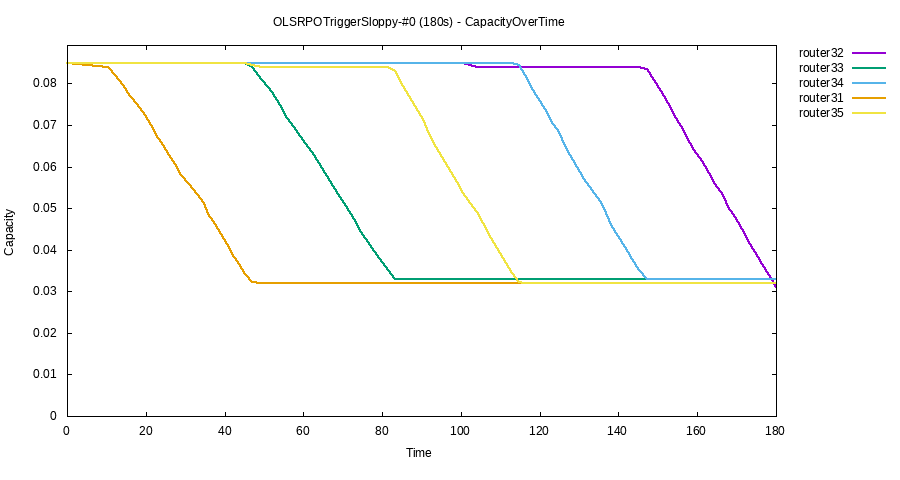
\includegraphics[scale=0.4]{bilder/os4.png} 
\captionof{figure}{Höherer Trigger $t=0.4$ bei OLSR-PO, 180 Sekunden}
\end{center}

\begin{center}
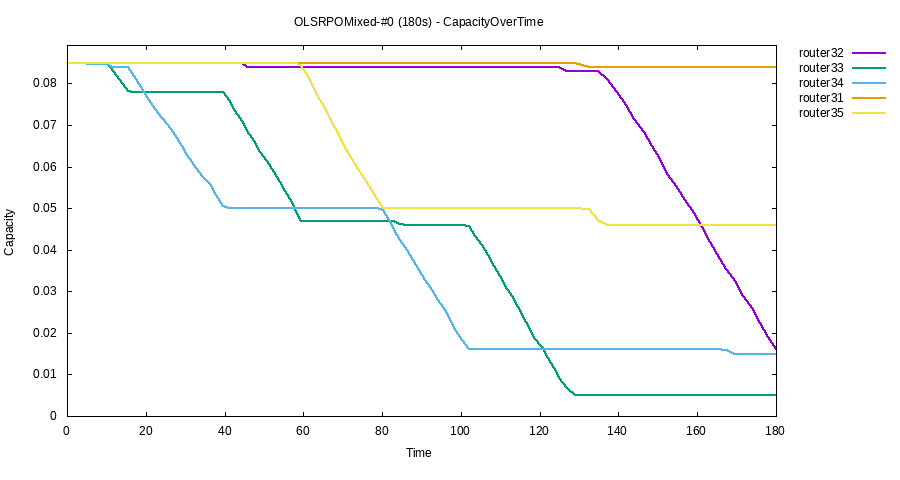
\includegraphics[scale=0.4]{bilder/os5.png} \\
\captionof{figure}{OLSR und OLSR-PO im Mischbetrieb, 180 Sekunden}
\end{center}


\chapter{Multi Hop}
\label{appendix:multihop}

\begin{center}
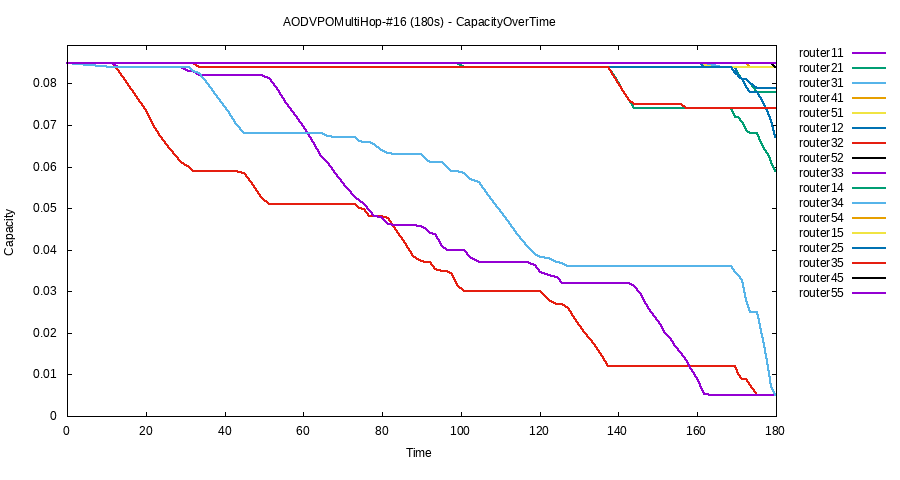
\includegraphics[scale=0.4]{bilder/m2.png} \\
\captionof{figure}{Verlauf Ladezustand bei AODV-PO im MutiHop Netz, 180 Sekunden}
\end{center}

\newpage

\begin{center}
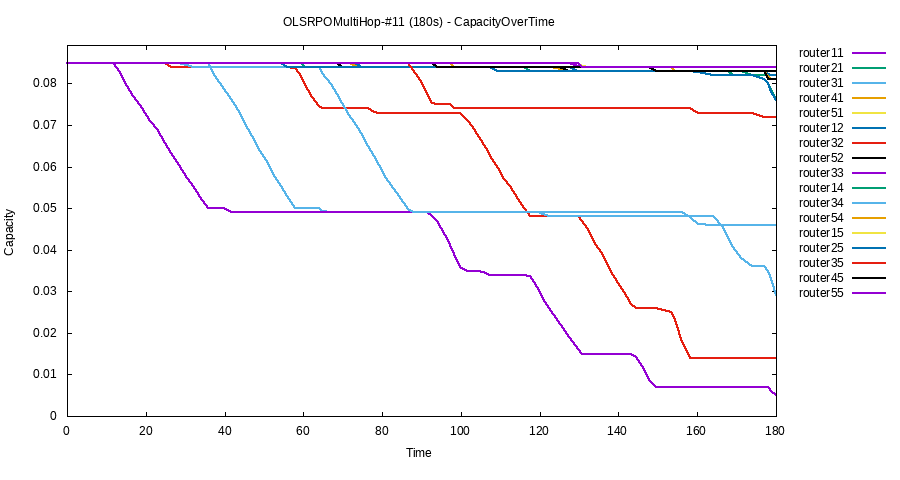
\includegraphics[scale=0.4]{bilder/m1.png} \\
\captionof{figure}{Verlauf Ladezustand bei OLSR-PO im MutiHop Netz, 180 Sekunden}
\end{center}

\chapter{Wiederholungen}
\label{appendix:repeat}

\begin{center}
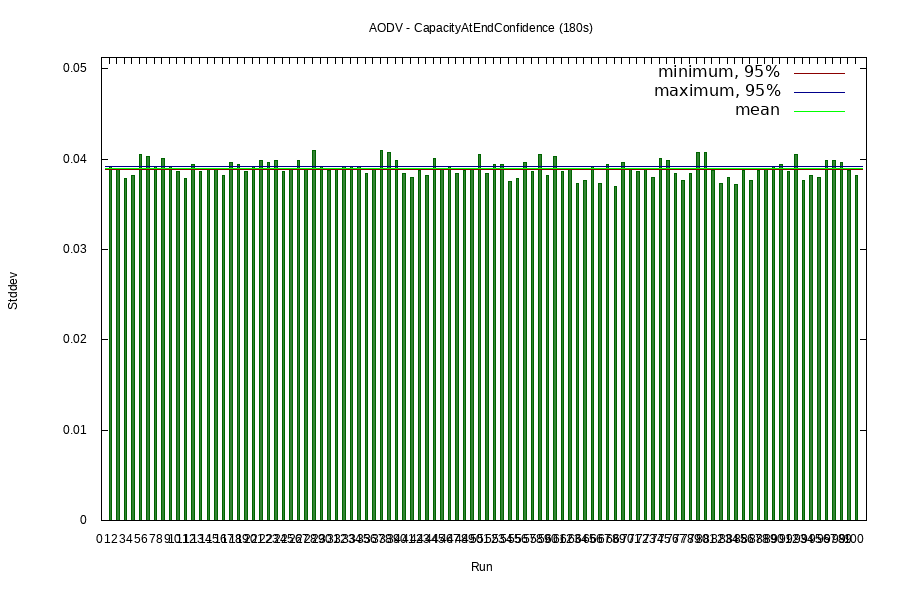
\includegraphics[scale=0.4]{bilder/sa4.png} \\
\captionof{figure}{Analyse Durchläufe AODV, 180 Sekunden}
\end{center}

\newpage

\begin{center}
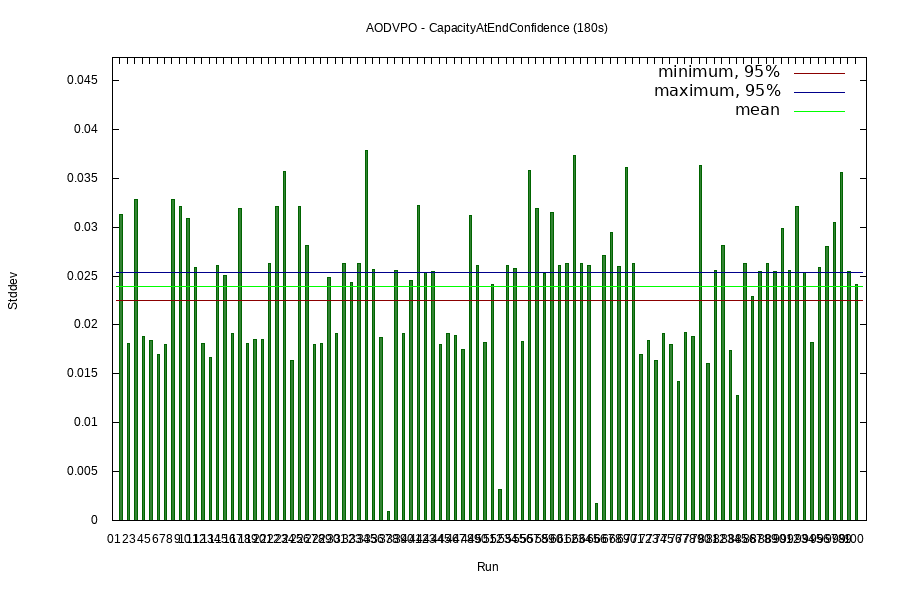
\includegraphics[scale=0.4]{bilder/sa5.png} \\
\captionof{figure}{Analyse Durchläufe AODV-PO, 180 Sekunden}
\end{center}

\begin{center}
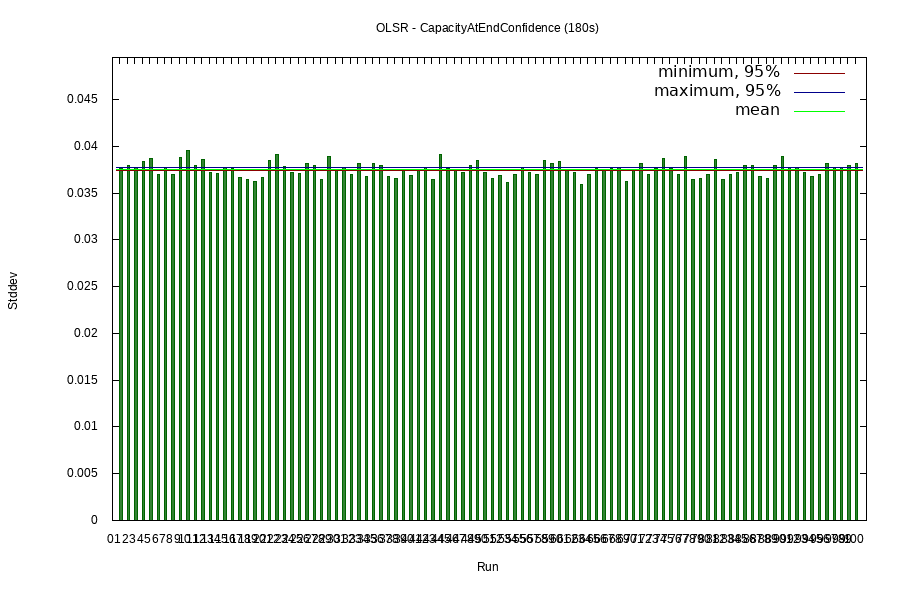
\includegraphics[scale=0.4]{bilder/so4.png} \\
\captionof{figure}{Analyse Durchläufe OLSR, 180 Sekunden}
\end{center}

\newpage

\begin{center}
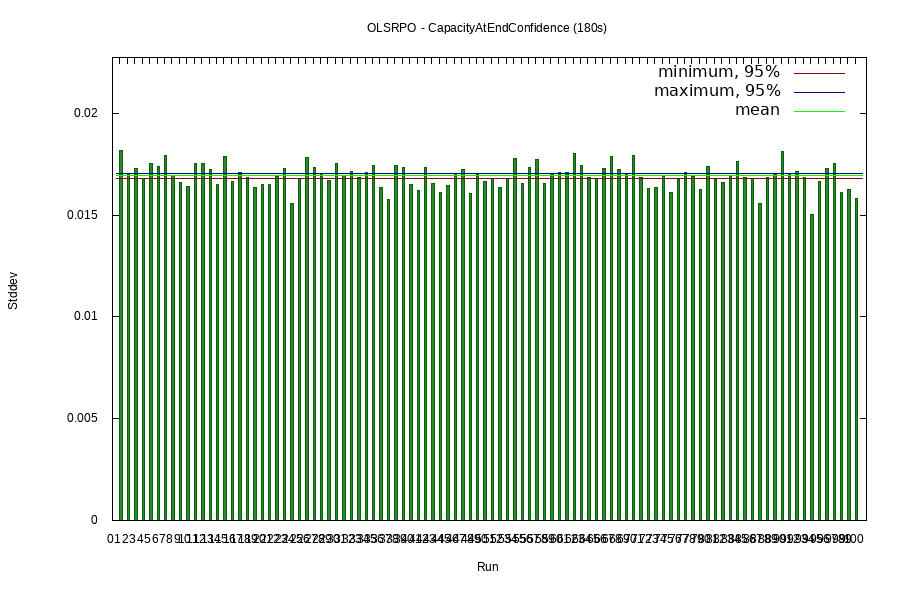
\includegraphics[scale=0.4]{bilder/so5.png} \\
\captionof{figure}{Analyse Durchläufe OLSR-PO, 180 Sekunden}
\end{center}

\chapter{3D Diagramme}
\label{appendix:3d}

\begin{center}
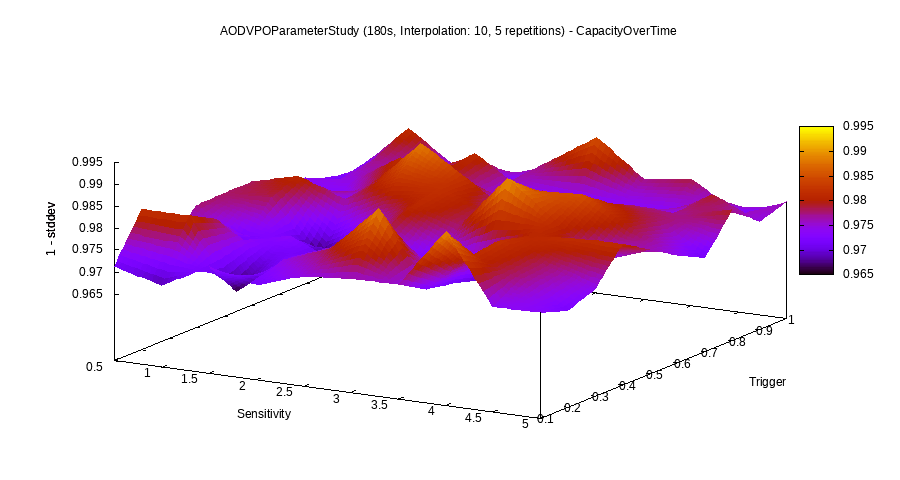
\includegraphics[scale=0.4]{bilder/o31.png} \\
\captionof{figure}{3D Darstellung Ladezustand ParameterStudy bei AODV, 180 Sekunden}
\end{center}

\newpage

\begin{center}
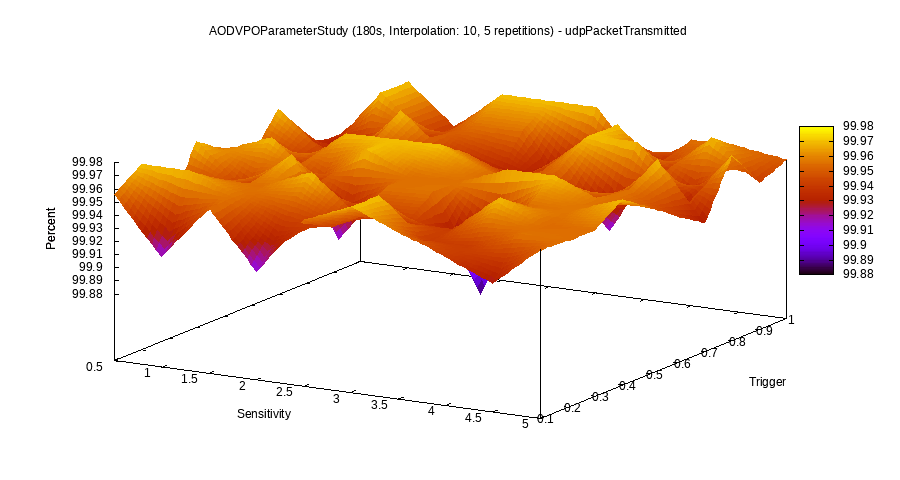
\includegraphics[scale=0.4]{bilder/o32.png} \\
\captionof{figure}{3D Darstellung PacketLoss ParameterStudy bei AODV, 180 Sekunden}
\end{center}

\begin{center}
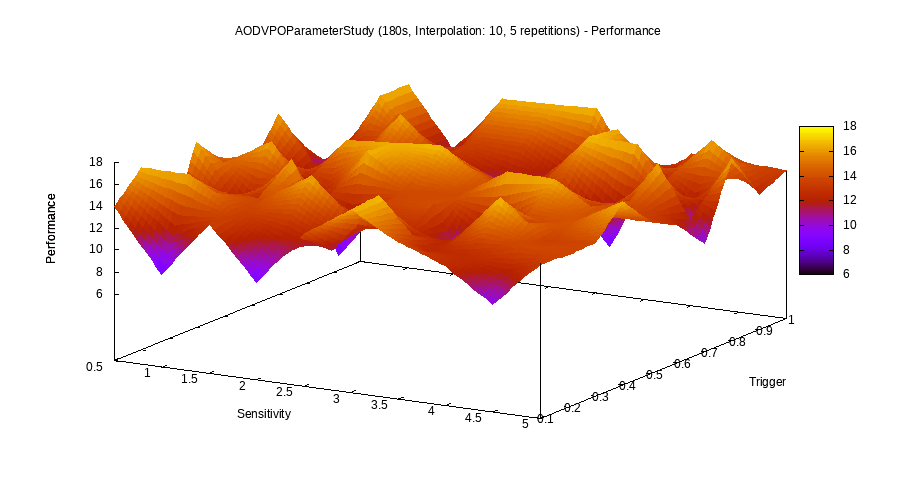
\includegraphics[scale=0.4]{bilder/o33.png} \\
\captionof{figure}{3D Darstellung Performance ParameterStudy bei AODV, 180 Sekunden}
\end{center}

\newpage

\begin{center}
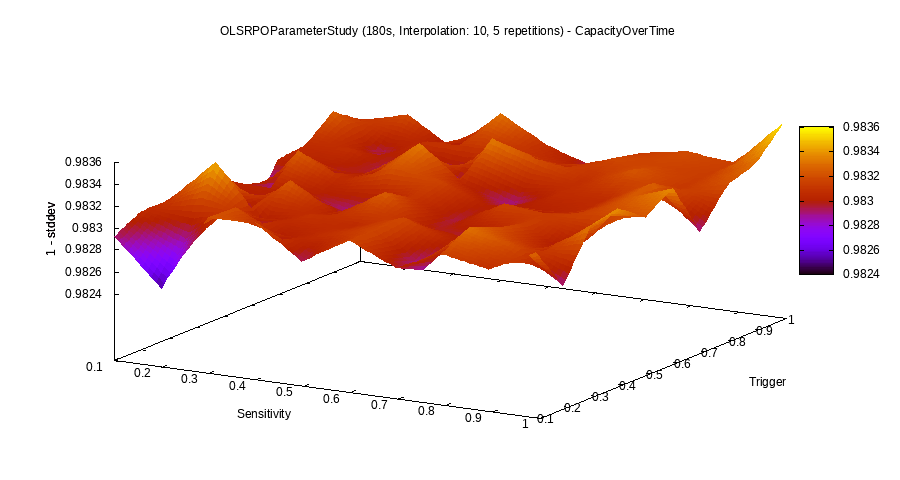
\includegraphics[scale=0.4]{bilder/o34.png} \\
\captionof{figure}{3D Darstellung Ladezustand ParameterStudy bei OLSR, 180 Sekunden}
\end{center}

\begin{center}
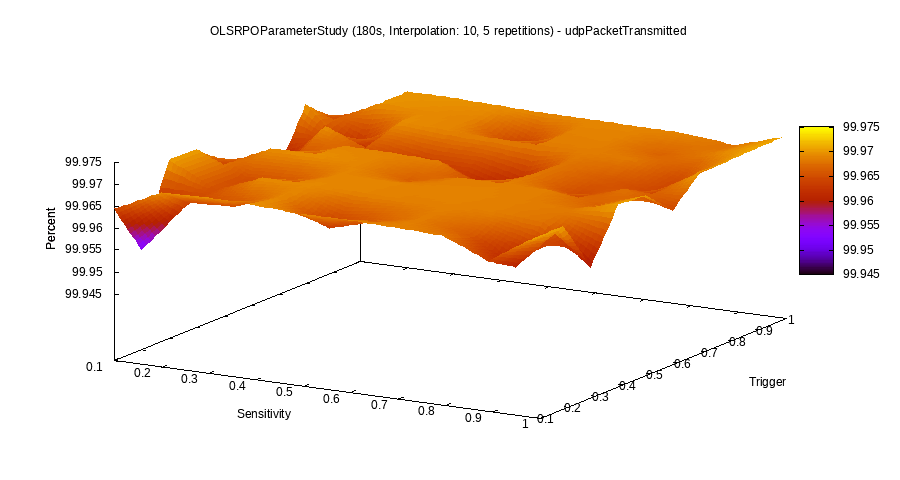
\includegraphics[scale=0.4]{bilder/o35.png} \\
\captionof{figure}{3D Darstellung PacketLoss ParameterStudy bei OLSR, 180 Sekunden}
\end{center}

\newpage

\begin{center}
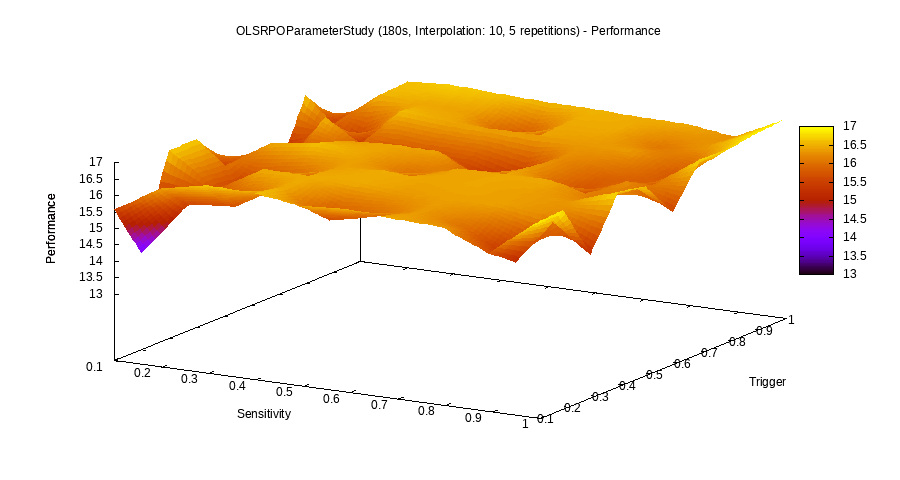
\includegraphics[scale=0.4]{bilder/o36.png} \\
\captionof{figure}{3D Darstellung Performance ParameterStudy bei OLSR, 180 Sekunden}
\end{center}

% glossar.tex
% Datendatei für die Glossareinträge

\usepackage[acronym,translate=babel]{glossaries}
\glstoctrue
\makeglossaries

\newcommand*{\newdualentry}[7][]{
  \newglossaryentry{main-#2}{name={#4},
  text={#3\glsadd{#2}},
  description={{#5}},
  long={#4},
  longplural={#6},
  plural={#7\glsadd{#2}},
  firstplural={{#6} ({#7})},
  #1
  }
  \newglossaryentry{#2}{
  type=\acronymtype,
  first={#4 (#3)},
  long={#4},
  longplural={#6},
  plural={#7\glsadd{main-#2}},
  firstplural={{#6} ({#7})},
  name={#3\glsadd{main-#2}},
  description={\glslink{main-#2}{#4}}
  }
}


\newcommand*{\newsingleentry}[5][]{
  \newglossaryentry{#2}{name={#3},
  text={#3},
  description={#4},
  plural={#5},
  #1
  }
}

%%%%%% ohne Akronym %%%%%%

\newsingleentry{rip}{Routing Information Protocol}{Ein Routing-Protokoll auf Basis des Distanzvektoralgorithmus, das innerhalb eines autonomen Systems (z. B. LAN) eingesetzt wird, um die Routingtabellen von Routern automatisch zu erstellen}{Routing Information Protocols}
\newsingleentry{ospf}{Open Shortest Path First}{Ein von der IETF entwickeltes Link-State-Routing-Protokoll}{Open Shortest Path First}
\newsingleentry{bgp}{Border Gateway Protocol}{Das im Internet eingesetzte Routingprotokoll}{Border Gateway Protocols}
\newsingleentry{igp}{Interior Gateway Protocol}{Routingprotokolle, die grundsätzlich für den Einsatz innerhalb geschlossener Netze, sogenannte Autonome Systeme, gedacht sind}{Interior Gateway Protocols}
\newsingleentry{egp}{Exterior Gateway Protocol}{Routingprotokolle, die grundsätzlich für Verbindung geschlossener Netze, sogenannte Autonome Systeme, gedacht sind}{Exterior Gateway Protocols}
\newsingleentry{iot}{Internet of Things}{Bezeichnet die Vision einer globalen Infrastruktur der Informationsgesellschaften, die es ermöglicht physische und virtuelle Gegenstände miteinander zu vernetzen und sie durch Informations- und Kommunikationstechniken zusammenarbeiten zu lassen}{Internets of Things}
\newsingleentry{smarthome}{SmartHome}{Dient als Oberbegriff für technische Verfahren und Systeme in Wohnräumen und -häusern in deren Mittelpunkt eine Erhöhung von Wohn- und Lebensqualität, Sicherheit und effizienter Energienutzung auf Basis vernetzter und fernsteuerbarer Geräte und Installationen sowie automatisierbarer Abläufe steht}{SmartHomes}
\newsingleentry{route}{Route}{Der gesamte Weg, den ein Paket durch ein Netzwerk wählt}{Routen}
\newsingleentry{router}{Router}{Netzwerkteilnehmer, der Pakete für andere Teilnehmer weiterleitet}{Router}
\newsingleentry{smartphone}{Smartphone}{Ein Smartphone ist ein Mobiltelefon (umgangssprachlich Handy), das erheblich umfangreichere Computer-Funktionalitäten und -konnektivität als ein herkömmliches Mobiltelefon zur Verfügung stellt}{Smartphones}
\newsingleentry{gpl}{GPL}{Die GNU General Public License (kurz GNU GPL oder GPL) ist die am weitesten verbreitete Softwarelizenz, die einem gewährt die Software auszuführen, zu studieren, zu ändern und zu verbreiten (kopieren)}{GPL}
\newsingleentry{met}{Metrik}{Im Netzwerkbereich definiert die Metrik ein numerisches Maß für die Güte einer Verbindung bei Verwendung einer bestimmten Route}{Metriken}
\newsingleentry{wlahm}{Ad-Hoc-Modus}{Ein Modus für ein Funknetzwerk, in dem die Teilnehmer direkt miteinander kommunizieren}{Ad-Hoc-Modi}
\newsingleentry{wlism}{Infrastruktur-Modus}{Ein Modus für ein Funknetzwerk, in dem die Teilnehmer über einen zentralen Accesspoint kommunizieren}{Infrastruktur-Modi}
\newsingleentry{maclayer}{Sicherungsschicht}{Die Sicherungsschicht soll die korrekte Übertragung von Frames auf Schicht 2 des OSI Modells zwischen zwei miteinander verbundenen Systemen bewerkstelligen}{Sicherungsschichten}
\newsingleentry{nwlayer}{Vermittlungsschicht}{Die Vermittlungsschicht sorgt bei leitungsorientierten Diensten für das Schalten von Verbindungen und bei paketorientierten Diensten für die Weitervermittlung von Datenpaketen}{Vermittlungsschichten}
\newsingleentry{olsrmessage}{OLSR Message}{Die Kontrollinformationen bei OLSR, die als Nutzlast der OLSR Pakete verschickt werden}{OLSR Messages}

%%%%%% BIS HIER HIN GEPRUEFT %%%%%%

%%%%%% mit Akronym %%%%%%
\newdualentry{iana}{IANA}{Internet Assigned Numbers Authority}{Eine Abteilung der ICANN und für die Zuordnung von Nummern und Namen im Internet, insbesondere von IP-Adressen, zuständig. Sie ist eine der ältesten Institutionen im Internet}{Internet Assigned Numbers Authorities}{IANAs}
\newdualentry{aodv}{AODV}{Ad-hoc On-demand Distance Vector}{Ein Verfahren zum Weiterleiten von Daten durch ein mobiles Ad-hoc-Netz. Das Protokoll gehört zu den topologiebasierten reaktiven Routingverfahren. Routen zu bestimmten Zielen werden erst bei Bedarf ermittelt. Das Protokoll wird in RFC 3561 beschrieben}{Ad-hoc On-demand Distance Vector}{AODV}
\newdualentry{accesspoint}{AP}{AccessPoint}{Gemeinsamer Zugangspunkt für die Teilnehmer innerhalb eines BSS im Infrastruktur-Modus}{AccessPoints}{APs}
\newdualentry{ip}{IP}{Internet-Protocol}{Das Internet Protocol ist ein in Computernetzen weit verbreitetes Netzwerkprotokoll und stellt die Grundlage des Internets dar. Es ist die Implementierung der Internetschicht des TCP/IP-Modells \bzw der Vermittlungsschicht des OSI-Modells. IP ist ein verbindungsloses Protokoll, das bedeutet bei den Kommunikationspartnern wird kein Zustand etabliert}{Internet-Protocols}{IPs}
\newdualentry{tcpip}{TCP/IP}{TCP/IP Protocol-Stack}{Eine Sammlung diverser Protokolle wie UDP, TCP uvm. für den Einsatz mit dem Internet-Protocol}{TCP/IP Protocol-Stacks}{TCP/IPs}
\newdualentry{ipv4}{IPv4}{Internet-Protocol V4}{Die derzeit dominante Version des Internet Protocols mit TCP in der Version 4. Es kommen Netzwerkadressen mit einer Länge von 4 mal 8 Bit zum Einsatz}{Internet-Protocols V4}{IPv4s}
\newdualentry{ipv6}{IPv6}{Internet-Protocol V6}{Eine neue Version des Internet Protocols, die derzeit aufgrund der Knappheit verfügbarer IPv4-Adressen eingeführt wird. Es kommen Adressen mit einer Länge von 8 mal 16 Bit zum Einsatz}{Internet-Protocols V6}{IPv6s}
\newdualentry{mesh}{MESH}{Vermaschtes Netz}{Ein Netz, das zwei oder mehr Endgeräte zu einem vermaschten Netz verbindet}{Vermaschte Netze}{MESHs}
\newdualentry{manet}{MANET}{mobiles Ad-Hoc Netzwerk}{MESHs, die sich selbständig aufbauen und konfigurieren, nennt man auch mobile Ad-hoc-Netze oder MANET}{mobile Ad-Hoc Netzwerke}{MANETs}
\newdualentry{olsr}{OLSR}{Optimized Link State Routing}{Ein Routingprotokoll für mobile Ad-hoc-Netze, das eine an die Anforderungen eines mobilen drahtlosen LANs angepasste Version des Link State Routing darstellt. Das Protokoll wird in dem RFC 3626 beschrieben}{Optimized Link State Routing}{OLSR}
\newdualentry{rfc}{RFC}{Request for Comments}{Request for Comments - eine Reihe technischer und organisatorischer Dokumente des RFC-Editors zum Internet (ursprünglich Arpanet), die am 7. April 1969 begonnen wurden}{Requests for Comments}{RFCs}
\newdualentry{rv}{RV}{Routingverfahren}{Ein Verfahren nach dem bestimmt wird, wie eine Nachricht zum Ziel geleitet wird und wie dieser Weg ermittelt wird}{Routingverfahren}{RVs}
\newdualentry{wlan}{WLAN}{Wireless LAN}{Drahtloses Netzwerk auf Basis von IEEE 802.11}{Wireless LANs}{WLANs}
\newdualentry{wmn}{WMN}{Wireless Mesh Network}{Vermaschtes, drahtloses Netzwerk auf Basis von WLAN}{Wireless Mesh Networks}{WMNs}
\newdualentry{bss}{BSS}{Basic Service Set}{Fundamentale Einheit eines Funknetzes bei WLAN. Es definiert eine Gruppe von Teilnehmern, die eine gemeinsame Koordinationsfunktion nutzen}{Basic Service Sets}{BSSs}
\newdualentry{ibss}{IBSS}{Independent Basic Service Set}{Ein BSS, dass von den Teilnehmern innerhalb eines WLAN Ad-Hoc Netzes aufgespannt wird}{Independent Basic Service Sets}{IBSSs}
\newdualentry{ess}{ESS}{Extended Service Set}{Ein Verbund mehrerer BSS über ein DS im WLAN Infrastruktur-Modus. Ein ESS kann über ein Portal an andere Netzwerke angeschlossen sein}{Extendes Service Sets}{ESSs}
\newdualentry{ds}{DS}{Distribution System}{Ein implementationsunabhängiges System, dass mehrere BSS im WLAN Infrastruktur-Modus miteinander verbindet}{Distribuntion Systems}{DSs}
\newdualentry{wds}{WDS}{Wireless Distribution System}{Ein Distribution System, das die Teilnehmer über IEEE 802.11 verbindet}{Wireless Distribuntion Systems}{WDSs}
\newdualentry{wsan}{WSAN}{Wireless Sensor and Actor Network}{Ein Netzwerk aus intelligenten Sensoren und Aktoren, die geografisch verteilt und über ein WLAN miteinander verbunden sind}{Wireless Sensor and Actor Networks}{WSANs}
\newdualentry{sta}{STA}{Station}{Teilnehmer in einem IEEE 802.11 Netzwerk (Clients), die nicht als AccessPoint arbeiten}{Stations}{STAs}
\newdualentry{hop}{HOP}{Netzwerkabschnitt}{Ein Hop ist ein Netzwerkabschnitt und wird als Zähleinheit benutzt. Die Anzahl an Hops sagt, über wie viele Netzwerk-Abschnitte die Datenpakete übertragen wird. Solche Netzwerk-Abschnitte können durch Router oder andere Knotenpunkte definiert sein}{Netzwerkabschnitte}{HOPs}
\newdualentry{mp}{MP}{Mesh Point}{Bei IEEE 802.11s ein Teilnehmer, der die Steuerung, Verwaltung und den Betrieb des MESH ermöglicht}{Mesh Points}{MPs}
\newdualentry{map}{MAP}{Mesh Access Point}{Bei IEEE 802.11s ein Teilnehmer, der die Voraussetzungen eines Mesh Points erfüllt und zusätzlich als Access Point für Stations dient}{Mesh Access Points}{MAPs}
\newdualentry{hwmp}{HWMP}{Hybrid Wireless Mesh Protocol}{Bei IEEE 802.11s eingesetzes Routingverfahren}{Hybrid Wireless Mesh Protocols}{HWMPs}
\newdualentry{mpp}{MPP}{Mesh Portal}{Bei IEEE 802.11s ein Teilnehmer, der die Voraussetzungen eines Mesh Points erfüllt und eine Anbindung an externe Netze, z.B. dem Internet bereitstellt, sofern diese nicht über IEEE 802.11 angebunden sind}{Mesh Portals}{MPPs}
\newdualentry{udp}{UDP}{User Datagram Protocol}{Ein minimales verbindungsloses Netzwerkprotokoll, das zur Transportschicht der Internetprotokollfamilie gehört}{User Datagram Protocols}{UDPs}
\newdualentry{tcp}{TCP}{Transmission Control Protocol}{Eine Familie von Netzwerkprotokollen. Sie wird wegen ihrer großen Bedeutung für das Internet auch als Internetprotokollfamilie bezeichnet. Die Identifizierung der am Netzwerk teilnehmenden Rechner geschieht über IP-Adressen}{Transmission Control Protocols}{TCPs}
\newdualentry{icmp}{ICMP}{Internet Control Message Protocol}{Ein Protokoll zur Übertragung von Statusinformationen und Fehlermeldungen zwischen IP-Netzknoten}{Internet Control Message Protocols}{ICMPs}
\newdualentry{uca}{UCA}{Unicast Address}{Eine IP-Adresse, die einen Teilnehmer bezeichnet}{Unicast Addresses}{UCAs}
\newdualentry{nwa}{NWA}{Network Address}{Eine IP-Adresse, die ein Subnetz bezeichnet}{Network Addresses}{NWAs}
\newdualentry{dsdv}{DSDV}{Destination-Sequenced Distance Vector}{Ein einfaches, auf dem Distanzvektoralgorithmus basierendes Routingverfahren}{Destination-Sequenced Distance Vector}{DSDVs}
\newdualentry{bca}{BCA}{Broadcast Address}{Eine IP-Adresse, die den Broadcast innerhalb eines Subnetzes bezeichnet}{Broadcast Addresses}{BCAs}
\newdualentry{rreq}{RREQ}{Route Request}{Eine Routenanforderung eines AODV Routers}{Route Requests}{RREQs}
\newdualentry{rrep}{RREP}{Route Reply}{Eine Antwort auf die Routenanforderung eines AODV Routers}{Route Replies}{RREPs}
\newdualentry{grrep}{GRREP}{Gratuitous Route Reply}{Eine Antwort auf die Gratuitous Routenanforderung eines AODV Routers}{Gratuitous Route Replies}{GRREPs}
\newdualentry{rerr}{RERR}{Route Error}{Die Meldung über die Nichtverfügbarkeit einer Route durch einen AODV Router}{Route Errors}{RERRs}
\newdualentry{rrepack}{RREP-ACK}{Route Reply Acknowledgement}{Die Bestätigung des Empfangs eines RREP durch einen AODV Router}{Route Reply Acknowledgements}{RREP-ACKs}
\newdualentry{mpr}{MPR}{Multipoint Relay}{Ein Host in einem OLSR Netz, der die Verteilung von Routinginformationen übernimmt. Jeder Teilnehmer bestimmt die Liste seiner MPRs selbst}{Multipoint Relays}{MPRs}
\newdualentry{midmessage}{MID message}{Multiple interface declaration message}{Informationen über die Adressen verschiedener Schnittstellen eines OLSR Hosts}{Multiple interface declaration messages}{MID messages}
\newdualentry{hellomessage}{HELLO message}{Hello message}{Informationen über die Interface Adressen eines OLSR Hosts}{Hello messages}{HELLO messages}
\newdualentry{tcmessage}{TC message}{Topology control message}{Informationen über die erreichbaren Nachbarn eines OLSR Hosts}{Topology control messages}{TC messages}
\newdualentry{1hnb}{1HNB}{One hop neighbour}{Ein direkter Nachbar eines OLSR Hosts}{One hop neighbours}{1HNBs}
\newdualentry{2hnb}{2HNB}{Two hop neighbour}{Ein direkter Nachbar des Nachbarn eines OLSR Hosts}{Two hop neighbours}{2HNBs}
\newdualentry{s2hnb}{S2HNB}{Strict two hop neighbour}{Ein direkter Nachbar des Nachbarn eines OLSR Hosts, ohne den Host selbst}{Strict two hop neighbours}{S2HNBs}
\newdualentry{dfw}{DFW}{default forwarding algorithm}{Der Standard-Algorithmus für die Weiterleitung von Nachrichten bei OLSR}{default forwarding algorithms}{DFWs}

%%%%%% BIS HIER HIN GEPRUEFT %%%%%%



% Abbildungsverzeichnis
\listoffigures
%\listoftables
\addcontentsline{toc}{chapter}{Abbildungsverzeichnis}
\cleardoublepage
% Algorithmenverzeichnis
%\listofalgorithms
%\addcontentsline{toc}{chapter}{Algorithmenverzeichnis}
%\cleardoublepage
% Literaturverzeichnis
%\bibliographystyle{gerplain}
\bibliographystyle{alpha}
\bibliography{literatur/bachelor}
\addcontentsline{toc}{chapter}{\bibname}
% Erklaerung
\thispagestyle{myheadings}
\markboth{}{ERKLÄRUNG}
\addcontentsline{toc}{chapter}{Erklärung}
% erklaerung.tex
% Eigenständigkeitserklärung

\cleardoublepage

%\chapter{Erklärung}
%\label{chapter:erklaerung}

\newpage
%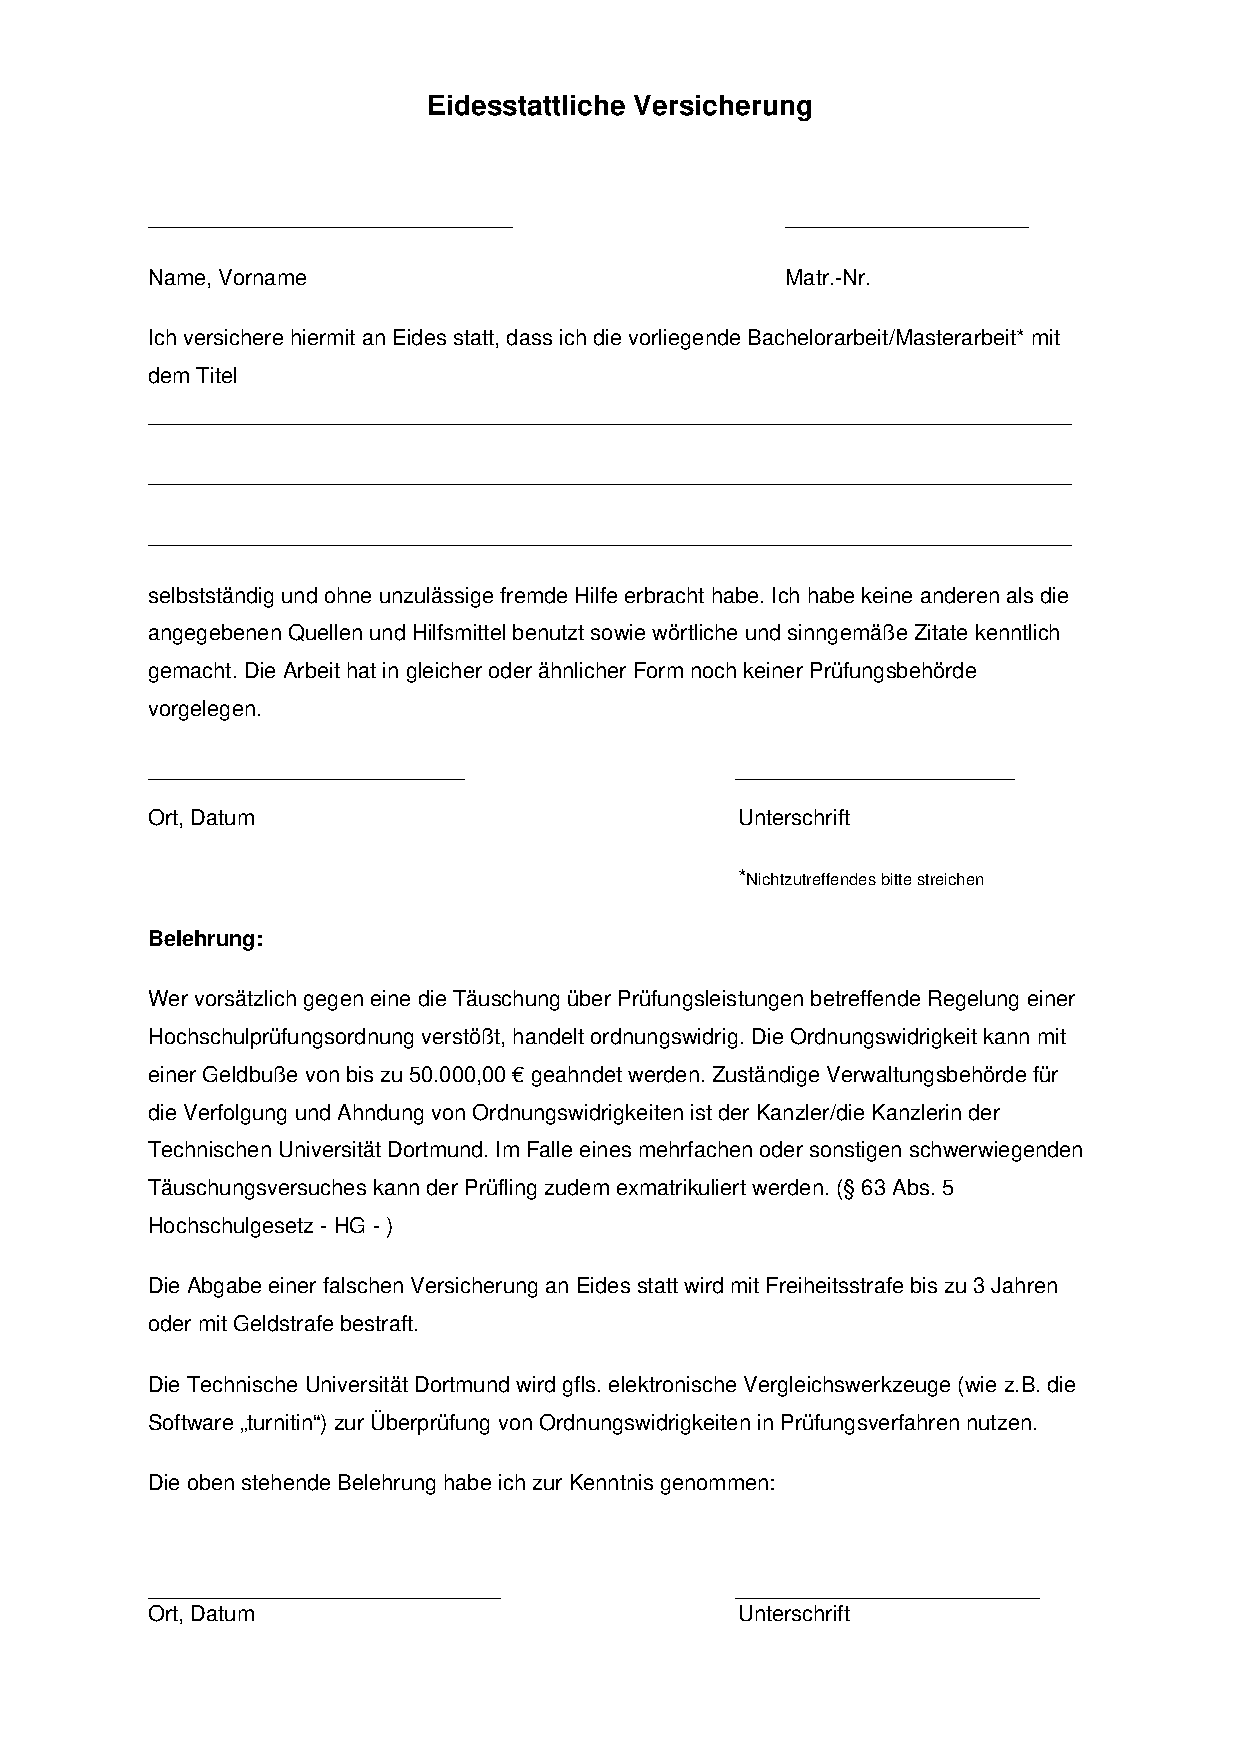
\includegraphics[scale=0.9]{bilder/eid.pdf}
\noindent\large{\textbf{Eidesstattliche Versicherung}}\newline

\noindent Hiermit versichere ich, Marcel Ebbrecht, Matrikel 111338, geboren am 09.11.1983 in Kassel, an Eides statt, dass ich die vorliegende Bachelorarbeit mit dem Titel \textbf{\glqq Energieeffizientes Routing in Ad-Hoc-Netzen - eine simulationsbasierte Analyse von OLSR und AODV\grqq}  selbstständig und ohne unzulässige, fremde Hilfe erbracht habe. Ich habe keine anderen als die angegebenen Quellen und Hilfsmittel benutzt sowie wörtliche und sinngemäße Zitate kenntlich gemacht. Die Arbeit hat in gleicher oder ähnlicher Form noch keiner Prüfungsbehörde vorgelegen. \newline\newline\newline

\noindent gez. Marcel Ebbrecht, Dortmund, der 01.04.2018\newline\newline\newline

\noindent{\textbf{Belehrung}}\newline\newline

\noindent Wer vorsätzlich gegen eine die Täuschung über Prüfungsleistung betreffende Regelung einer Hochschulprüfungsordnung verstößt, handelt ordnungswidrig. Die Ordnungswidrigkeit kann mit einer Geldbuße von bis zu 50000 Euro geahndet werden. Zuständige Verwaltungsbehörde für die Verfolgung und Ahndung von Ordnungswidrigkeiten ist der Kanzler / die Kanzlerin der Technischen Universität Dortmund. Im Falle eines mehrfachen oder sonstigen schwerwiegenden Täuschungsversuches kann der Prüfling zudem exmatrikuliert werden (§63 Abs.5 Hochschulgesetz - HG). Die Angabe einer falsches Versicherung an Eides statt wird mit Freiheitsstrafe von bis zu 3 Jahren oder mit Geldstrafe bestraft. Die Technische Universität Dortmund wird ggfs. technische Vergleichswerkzeuge (wie \zB die Software \glqq turnitin\grqq) zur Überprüfung von Ordnungswidrigkeiten in Prüfungsverfahren nutzen. Die oben stehende Belehrung habe ich zur Kenntnis genommen.\newline\newline\newline

\noindent gez. Marcel Ebbrecht, Dortmund, der 01.04.2018\newline\newline\newline



%\normalsize
%Hiermit versichere ich, dass ich die vorliegende Arbeit selbstständig verfasst \newline habe und keine anderen als die angegebenen %Quellen und Hilfsmittel verwendet sowie Zitate kenntlich gemacht habe.\\\\
%Dortmund, den \today \\\\\\\\ \newline
%Marcel Ebbrecht
% EOF
\cleardoublepage
\end{document}

